% \documentclass[11pt]{article}
\RequirePackage{fix-cm}

%%%%%%% To Springer
%\documentclass{svjour3}                     % onecolumn (standard format)
%\documentclass[smallcondensed]{svjour3}     % onecolumn (ditto)
\documentclass[smallextended,numbook,nospthms]{svjour3}
%\documentclass[smallextended,envcountsect,envcountsame,numbook]{svjour3}
\usepackage[12pt]{extsizes}
\setcounter{tocdepth}{4}
\setcounter{secnumdepth}{4}
\smartqed 

\makeatletter
\def\cl@chapter{}
\makeatother
\usepackage[utf8]{inputenc}
\usepackage{lmodern}
\usepackage[pdfpagelabels,colorlinks]{hyperref}
\usepackage{mathtools,amsfonts,amssymb,amscd,amsthm}
\usepackage[misc]{ifsym}
\usepackage[capitalize,nameinlink]{cleveref}
\usepackage{autonum}
\usepackage{cite}
% \usepackage{xcolor}
\crefname{equation}{}{}
%%--- LISTS ---%%%%%%%%%%%%%%%%%%%%%%%%%%%%%%%%%%%%%%%%%%%%%%%%%%%%%%%%%%%%%%%%%%%%%%%%%%%%%%%
\usepackage[shortlabels]{enumitem}
\newlist{lista}{enumerate}{1}
\setlist[lista]{label=\alph*., nosep,leftmargin=*,align=right}

\newlist{listi}{enumerate}{1}
\setlist[listi]{label={\upshape(\roman*\upshape)},leftmargin=*,align=right, widest=iii}

\usepackage{lmodern}
\usepackage{amssymb}
% \usepackage{amsthm}
\usepackage{dsfont}
\usepackage[pdftex,dvipsnames]{xcolor}
\setlength{\marginparwidth}{2cm}
\usepackage[colorinlistoftodos,prependcaption,textsize=tiny]{todonotes}
\reversemarginpar 

\usepackage{tkz-euclide,tkz-fct}

\usepackage{graphicx}
\graphicspath{{figures/}}
\usepackage{subfig}

\oddsidemargin=0pt
\evensidemargin=0pt
\textwidth=6.2in

\renewcommand{\baselinestretch}{1.0}

\headsep=1cm
\theoremstyle{plain}
\newtheorem{theorem}{Theorem}[section]
\newtheorem{lemma}[theorem]{Lemma}
\newtheorem{fact}[theorem]{Fact}
\newtheorem{proposition}[theorem]{Proposition}
\newtheorem{corollary}[theorem]{Corollary}
\newtheorem*{assumption}{Assumption EB}
% \newtheorem*{assumption}{Assumption EB}
\theoremstyle{definition}
\newtheorem{definition}[theorem]{Definition}
\Crefname{fact}{Fact}{Facts}
%\newtheorem*{pf}{Proof}

\Crefname{figure}{Figure}{Figures}

%\newcommand{\NN}{\ensuremath{\mathds N}}
\def\RR{\mathds R}
\def\NN{\mathds N}
\def\ZZ{\mathds Z}
\def\lV{\left\lVert }
\def\rV{\right\rVert }
\def\lv{\left\lvert }
\def\rv{\right\rvert}
\def\al{\alpha}
\def\be{\beta}
\def\ga{\gamma}
\DeclareMathOperator{\Id}{Id}
\DeclareMathOperator{\Fix}{Fix}
\DeclareMathOperator{\aff}{aff}
\DeclareMathOperator{\dist}{dist}
\DeclareMathOperator{\dom}{dom}
\DeclareMathOperator{\inte}{int}
\DeclareMathOperator{\bound}{bd}
\DeclareMathOperator{\epi}{epi}
\newcommand{\norm}[1]{\left\lVert#1\right\rVert}
\newcommand{\scal}[2]{\left\langle{#1},{#2}  \right\rangle}
\DeclareMathOperator{\circum}{circ}
\newcommand{\MAP}{{\rm MAP}}
\newcommand{\DRM}{{\rm DRM}}
\newcommand{\CRM}{{\rm CRM}}
\newcommand{\CARM}{{\rm CARM}}
\newcommand{\AMAP}{{\rm AMAP}}

\usepackage[left,mathlines]{lineno}
\usepackage{etoolbox} %% <- for \pretocmd, \apptocmd and \patchcmd
%% Patch AMS math environment:
\newcommand*\linenomathpatchAMS[1]{%
  \expandafter\pretocmd\csname #1\endcsname {\linenomathAMS}{}{}%
  \expandafter\pretocmd\csname #1*\endcsname{\linenomathAMS}{}{}%
  \expandafter\apptocmd\csname end#1\endcsname {\endlinenomath}{}{}%
  \expandafter\apptocmd\csname end#1*\endcsname{\endlinenomath}{}{}%
}

%% Definition of \linenomathAMS depends on whether the mathlines option is provided
\expandafter\ifx\linenomath\linenomathWithnumbers
  \let\linenomathAMS\linenomathWithnumbers
  %% The following line gets rid of an extra line numbers at the bottom:
  \patchcmd\linenomathAMS{\advance\postdisplaypenalty\linenopenalty}{}{}{}
\else
  \let\linenomathAMS\linenomathNonumbers
\fi

% \linenomathpatch{equation} %% <- unnecessary, equation is already patched
\linenomathpatchAMS{gather}
\linenomathpatchAMS{multline}
\linenomathpatchAMS{align}
\linenomathpatchAMS{alignat}
\linenomathpatchAMS{flalign}

%\linenumbers

\usepackage{pdfpages}

\title{Dissertação - Novo}
\author{guilhermehm.araujo }
\date{March 2021}

\begin{document}
\thispagestyle{empty}
\begin{center}
\textbf{\LARGE Fundação Getulio Vargas}\\ 
\textbf{\LARGE Escola de Matemática Aplicada}

\par
\vspace{170pt}
\textbf{\Large Guilherme Henrique Macieira de Araújo}\\
\vspace{32pt}
\textbf{\Large Circumcentering outer-approximate projections and reflections for the convex feasibility problem}\\
\end{center}

\par
\vfill
\begin{center}
{{\normalsize Rio de Janeiro}\\
{\normalsize \the\year}}
\end{center}

\newpage
\thispagestyle{empty}

\newpage
\begin{center}
\textbf{\LARGE Guilherme Henrique Macieira de Araújo}

\par
\vspace{200pt}
\textbf{\Large Circumcentering outer-approximate projections and reflections for the convex feasibility problem}
\end{center}

\par
\vspace{85pt}
\hspace*{175pt}\parbox{7.6cm}{{\normalsize Dissertação submetida à Escola de Matemática Aplicada como requisito parcial para a obtenção do grau de Mestre em Modelagem Matemática}}

%\par
%\vspace{1em}
%\hspace*{125pt}\parbox{10.0cm}{{\normalsize Área de Concentração: xx}}

\par
\vspace{1em}
\hspace*{125pt}\parbox{10.0cm}{{\normalsize Orientador: Roger Behling}\\
{\normalsize Co-Orientador: Luiz Rafael Santos}}

\par
\vfill
\begin{center}
{{\normalsize Rio de Janeiro}\\
{\normalsize \the\year}}
\end{center}

\thispagestyle{empty}


\newpage

\thispagestyle{empty}
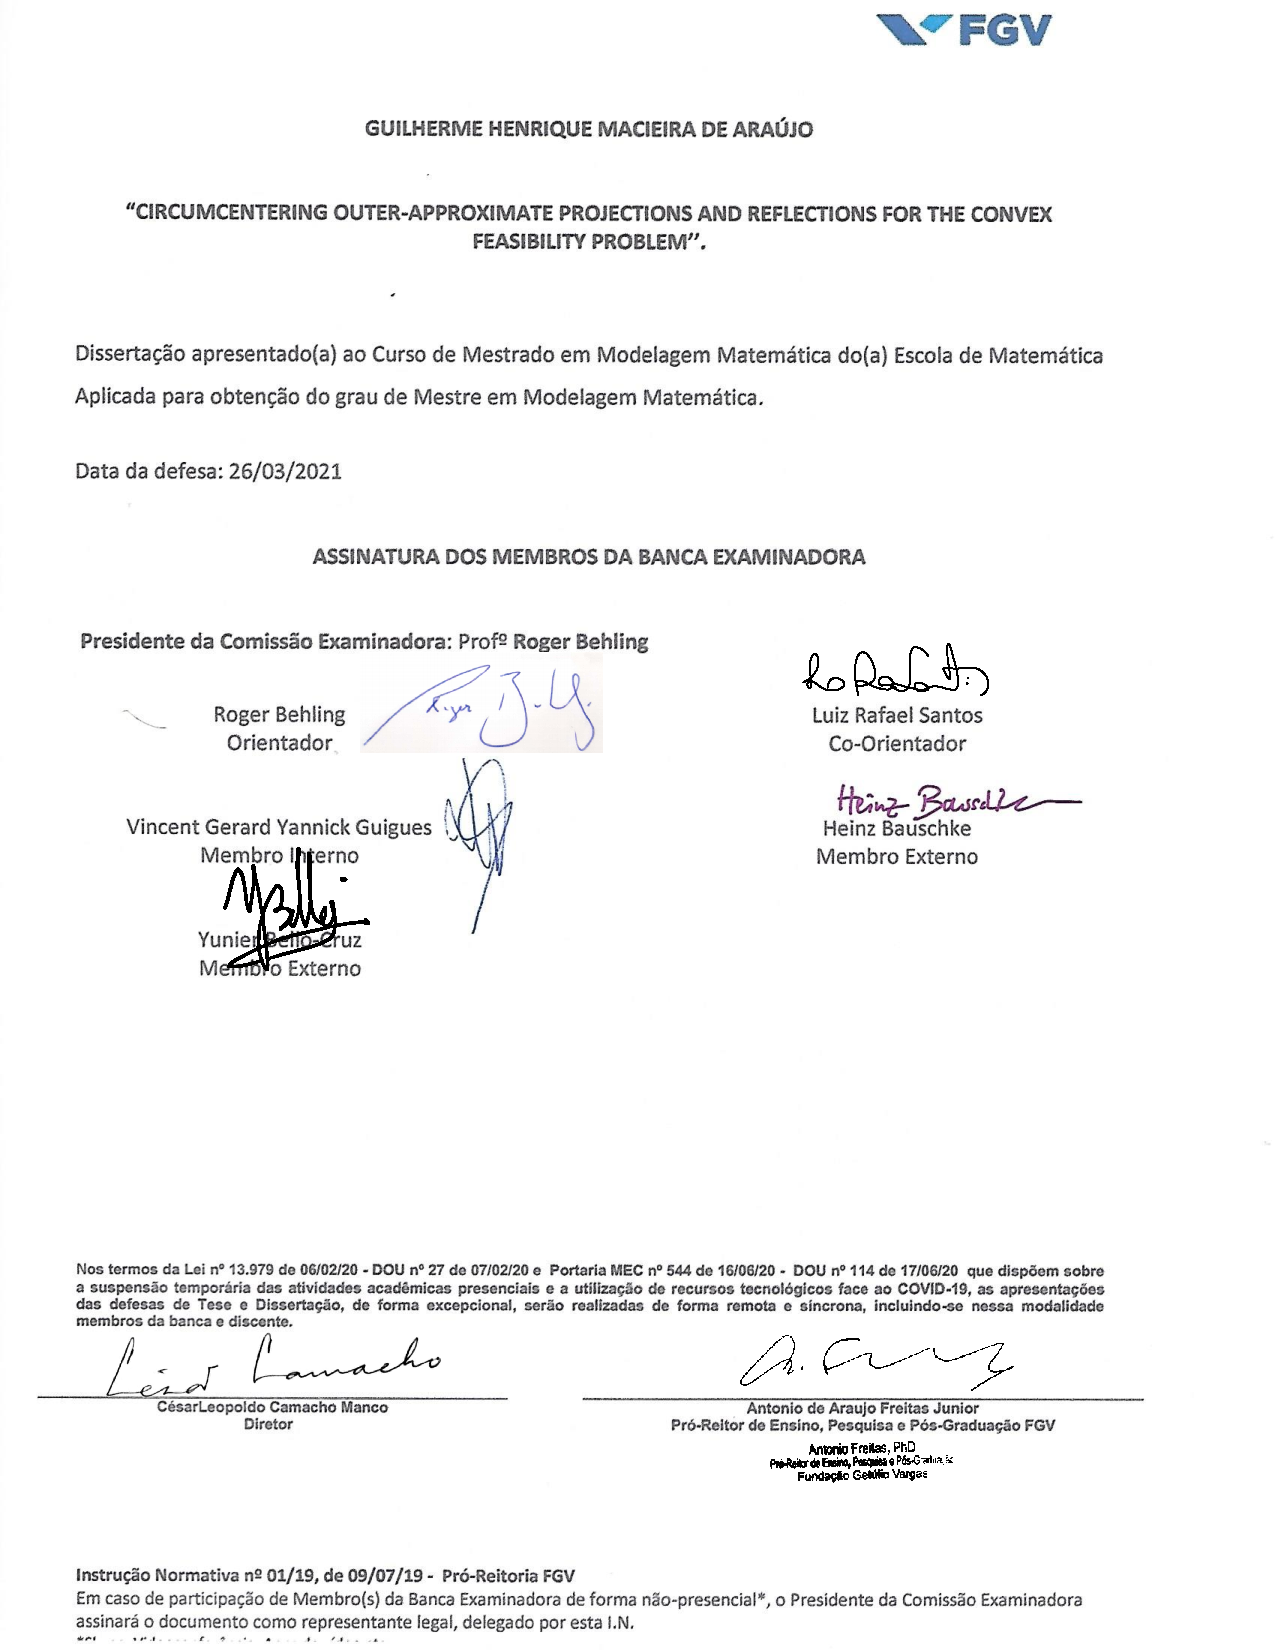
\includepdf[pages=-,offset=0 0]{Aprov. Banca - Guilherme Macieira.pdf}

\thispagestyle{empty}

\newpage
\begin{center}
\textbf{\normalsize Abstract}
\end{center}
\vspace{1pt}

Recently, circumcenter schemes were  applied to solving general convex feasibility problems. In order to overcome costly computations of projections and reflections onto convex sets, we present a variant of the circumcentered-reflection method which employs outer-approximate projections, inspired by Fukushima.
With a very practical appeal, this  notion relies on separating hyperplanes and is considered in our hybrid method for finding a point in the intersection of finitely many convex sets.  We derive convergence in general, linear convergence under an error bound condition, and present successful numerical experiments.

Keywords: circumcenters, approximate projections, convex feasibility problem, alternating projections, Douglas-Rachford method

\newpage
\thispagestyle{empty}

\listoffigures

\listoftables

\newpage

\thispagestyle{empty}

\newpage
\tableofcontents
\thispagestyle{empty}

\newpage
\section{Introduction}
We consider the convex feasibility problem (CFP) of finding a point in a nonempty set given by the intersection of finitely many closed convex sets. We are going to reduce CFP to seeking a point common to a closed convex set and an affine subspace, referred to as CFP-red. This reduction in the number of target sets embeds CFP by means of Pierra's product space reformulation \cite{Pierra:1984hl}. Also, feasibility sets of general convex optimization problems are standardly split into convex inequalities and affine equalities, which define a closed convex set and an affine subspace, respectively.

%In addition to being important on its own, CFP-CA covers central classes of feasibility problems. For instance, the general CFP of finding a point in the intersection of finitely many closed convex sets 
%$\{K_i\}_{i=1}^{m} \subset\RR^{p}$
%$\mathrm{K}\coloneqq K_1 \times\dots\times K_m\subset\RR^{pm}$
%$\mathrm{U}\coloneqq\{(x,\dots,x)\mid x\in\RR^p\}\subset\RR^{pm}$. 


%This approach is known as Pierra's product space formulation~\cite{Pierra:1984hl}. Also, convex optimization problems standardly have a feasible set of the form  $K\cap U$, with $K\coloneqq\{x\in\RR^{n} \mid g(x)\leq 0\}$ and $U\coloneqq \{x\in\RR^{n} \mid Ax=b\}$, where $g:\RR^{n}\longrightarrow\RR^{q}$ is a convex function, $A\in\RR^{r\times n}$ is a matrix and $b\in\RR^{r}$.

Projection-based methods are usually utilized for solving CFP. Widely known are the Method of Alternating Projections (MAP), the Douglas-Rachford method (DRM) and the Cimmino method \cite{Cimmino:1938tp}. Recently, the the Circumcentered-Reflection method (CRM) has been developed as a powerful new tool for solving CFP, outperforming MAP and DRM. It was introduced in \cite{Behling:2018a,Behling:2018} and further enhanced in \cite{Arefidamghani:2020,Bauschke:2018ut,Bauschke:2018wa, Bauschke:2019uh,Bauschke:2020a,Behling:2019dj,Behling:2020,Dizon:2019vq,Dizon:2020a,Ouyang:2018gu,Lindstrom:2020a}. 

In its debut in \cite{Behling:2018a,Behling:2018}, CRM was shown to solve the best approximation problem for finitely many affine subspaces with linear convergence. Following these first results, \cite{Behling:2019dj}, a block-wise variant of CRM was introduced, which also converges linearly for affine subspaces (in one step if the subspaces are hyperplanes) and can also be seen as a generalization of MAP. CRM was later shown in \cite{Behling:2020} to converge to a solution of CFP-red and it was proven in \cite{Arefidamghani:2020} that linear convergence is obtained in the presence of an error bound condition.

More recently, some contributions to CRM have been presented by scholars other than the original authors, some of which we outline here. In \cite{Bauschke:2019uh,Bauschke:2020a}, the authors generalize CRM for isometries and provide conditions for weak and linear convergence of the derived Circumcentered Isometry Method (CIM); in \cite{Dizon:2019vq} CRM is shown to converge locally in some nonconvex settings (outperforming DRM) and to compare favorably to Newton-Raphson method as a root solver and in \cite{Dizon:2020a}, the CRM is also employed for solving wavelet feasibility problems.

Nevertheless, these algorithms rely on the computation of exact orthogonal projections. One has to bear in mind though that, context depending, this task alone might be as hard as the original problem itself. In this regard, we present in this work a version of CRM employing \emph{outer-approximate projections}. 

The outer-approximate projections we are going to consider, formally given in \Cref{def:approx proj}, are more tractable than the exact ones while still enjoying some of their properties. This notion is based on the paper~\cite{Fukushima:1983} by Fukushima from 1983.  We prove that employing these outer-approximate projections within CRM preserves the convergence results from \cite{Behling:2020} and, under a Lipschitzian error bound, linear convergence as in \cite{Arefidamghani:2020} is maintained as well. In this view, the results shown here are a paramount of the aforementioned works \cite{Behling:2020, Arefidamghani:2020}. Our method will be referred to as Circumcentered-Approximate Reflection Method (CARM). Despite featuring outer approximations,  CARM performs competitively to CRM in our numerical experiments. 

This paper is organized as follows. In \cref{sec:prelim}, we recall concepts such as convexity, nonexpansivity, Fejér monotonicity, Q and R-linear convergence and the characterization of circumcenters, while stating and proving facts relevant to the problems and methods of our interest. In \cref{sec:proj methods}, we state Pierra's product space reformulation and review MAP, DRM and CRM, while proving key convergence results and presenting variants. In \cref{sec:approx proj}, we present our notion of outer-approximate projection as well as other notions of approximating orthogonal projections. In \cref{sec:CARM}, we introduce CARM and prove its convergence. For the sake of completeness, we carry out a similar study for a corresponding outer-approximate MAP (AMAP) in \cref{sec:AMAP}, in view of numerical comparisons with CARM. \cref{sec:comp} features a theoretical comparison between CARM and AMAP and their behavior under an error bound condition. In the presence of an error bound, both CARM and AMAP converge linearly to a solution of CFP-red with CARM having a better linear rate than AMAP. \cref{sec:numerical} contains exploratory numerical experiments, considering problems where exact projections are available and comparing CARM with CRM (as well as MAP and AMAP). In these experiments, CARM performs successfully. \cref{sec:remarks} presents concluding remarks.

\newpage
\section{Preliminary concepts}\label{sec:prelim}
The aim of this section is to familiarize the reader with the concepts of convexity, projections, fixed-point operators and circumcenters, as well as ancillary theory.     

This dissertation is intended to be self-contained, except for the use of some well-known results in calculus and analysis. By facts, we denote propositions, theorems, lemmas and corollaries that have been first presented and proven in previously published works; a small subset of their proofs, mostly of auxiliary technical results, will be omitted, in which case the original proof will be referred to.

It follows that all statements denoted as propositions, theorems, lemmas and corollaries are new to this work. For ease of reading and understanding, however, definitions will be called as such regardless of their authorship, though context is sufficient for determining whether they are new to this work or not.

While this work's definitions, facts and propositions will be presented with respect to $\RR^n$, a great deal can be generalized to a Hilbert space $\mathcal{H}$ with extended-reals-valued functions (see \cite{BC2011, Rockafellar:1996}, for reference). In this more general setting, it is often required that functions be lower semicontinuous throughout and proper. The function $f:\mathcal{X} \rightarrow [-\infty,+\infty]$, where $\mathcal{X}$ is nonempty, is lower semicontinuous if, for every net $\left(x_{a}\right)_{a \in A}$ in $\mathcal{X}$, $x_{a} \rightarrow x \Rightarrow f(x) \leq \liminf \left(x_{a}\right)$; it is proper if there exists at least one $x \in \mathcal{X}$ such that  $f(x)<+\infty$ and $f(x)>-\infty$ for all $x \in \mathcal{X}$.  For more on this, see \cite[Sections 7 and 30]{Rockafellar:1996} and \cite[Chapter 1 and 9]{BC2011}, among others.

First, we fix notation and recollect some basic facts. 
\subsection{Notation}
Throughout the paper, $\scal{\cdot}{\cdot}$ stands for the Euclidean inner product and its induced  norm $\norm{\cdot}\coloneqq\sqrt{\scal{\cdot}{\cdot}}$. The nonnegative integer numbers will be denoted by $\NN$, the nonnegative real numbers by $\RR_{+}$ and the positive real numbers by $\RR_{++}$. The distance between a point $x\in\RR^{n}$ and a set $X\subset \RR^{n}$ is given by $\dist(x,X)\coloneqq \inf_{y\in X} \norm{x-y}$. We denote the set of fixed points of the operator $T$ by $\Fix T$, where $\Fix T := \{x \mid T(x)=x\}$. By $\rightarrow$ we represent a single-valued relationship, while $\rightrightarrows$ represents a set-valued relationship. $(x^k)_{k \in \NN}$ denotes the sequence $\{x^0, x^1, \ldots\}$. By $B(x;r)$ we denote an open ball with center $x$ and radius $r$. By $\triangle{[A, B, C]}$ we denote a triangle with vertices $A$, $B$ and $C$, and by $\angle{[A, B, C]}$ we denote the angle formed by the sides $AB$ and $BC$. When we take a limit $x \rightarrow 0+$, we mean that $x$ approaches 0 from the positive side, while $x \rightarrow 0-$ means that $x$ approaches 0 from the negative side. By $f(t)=o(t)$ we denote a function $f:\RR_{+} \rightarrow \RR$ with the property that $f(t)/t \rightarrow 0$ when $t \rightarrow 0+$. By $\operatorname{cl} X$ we denote the closure of the set $X$ and by $\operatorname{bdry} X$ we denote the boundary of $X$.

\subsection{Convex sets}
We begin by reminding the fundamental notion of convex sets.
\begin{definition}[Convex sets]\label{def:convex}
	A subset $K$ of $\RR^n$ is a \emph{convex set} if for all $\alpha \in [0,1]$, for all $x,y \in K$ we have that $\alpha x + (1-\alpha)y \in K$. In particular, $\RR^n$ and $\varnothing$ are convex.
	\end{definition}

Many properties about convex sets can be derived straight from its definition, e.g. that the finite sum of convex sets is convex. While we will not state all properties of convex sets, we will state a few in particular which will be used in further proofs and arguments.

Though these facts are very well-established and are likely to be found in any convex optimization textbook, notation, hypotheses and order of presentation (consequently, previously proven facts) may vary slightly depending on the source. For the sake of internal consistency, we will follow mostly along the lines of \cite{Izmailov:2014} for facts on convex sets and functions.

The first fact we will present is that the intersection of convex sets is also a convex set.

\begin{fact}[Intersection of convex sets is convex]\label{fact:cap convex}
Let $K_i \subset \RR^n$, $i \in I$ (where $I$ is a possibly infinite set), be convex sets. Then the intersection $K=\cap_{i \in I}K_i$ is also a convex set.
\end{fact}	
\begin{proof}
	Let $x \in K$ and $y \in K$. From the definition of intersection, $x \in K_i$ and $y \in K_i$ for all $i \in I$. Since the sets $K_i$ are convex, $\alpha x + (1-\alpha)y \in K_i$ for any $\alpha \in [0,1]$ and all $i \in I$. Thus, by the definition of intersection, $\alpha x + (1-\alpha)y \in K$. Hence, $K$ is convex.
\end{proof}

One characterization of convex sets is that a set is convex if, and only if, it contains all convex combinations of its points. This statement, as well as the definition of convex combination, is presented below.
\begin{fact}[Convex combination characterization of convex sets]\label{fact:convex conv comb}
	A set $K \subset \RR^n$ is convex if, and only if, for any $p \in \{1,2,\ldots\}$, $x^{i} \in K$ and $\alpha_{i} \in [0,1]$, $i=1,\ldots,p$, such that $\sum_{i=1}^{p}\alpha_{i}=1$, the \emph{convex combination} $\sum_{i=1}^{p} \alpha_{i}x^{i} \in K$.
\end{fact}
\begin{proof}
	If $K$ contains every convex combinations of its points, in particular it contains the convex combinations of any two points (that is, for $p=2$). Thus, $K$ is convex by \cref{def:convex}.
	
	Assume now that $K$ is convex. The proof is done by induction with respect to the number of points $p \in \NN$. For given $p \in \NN$ and $x^{i} \in K$, $\alpha_{i} \in [0,1]$, $i=1,\ldots,p$ such that $\sum_{i=1}^{p} \alpha_{i}=1$, we define $x=\sum{i=1}^{p} \alpha_{i}x^{i}$.
	For the base step, if $p=1$, we have that $\alpha_{1}=1$ and, thus, $x=x^{1} \in K$.
	Now, suppose any convex combination of $j \geq 1$ points of $K$ belongs to $K$, and consider the case $p=j+1$.
	If $\alpha_{j+1}=1$, then $\alpha_{i}=0$ for all $i=1,\ldots,j$. In this case, $x=x^{j+1} \in K$.
	Let $\alpha_{j+1} \in [0,1)$. Since $1-\alpha_{j+1}>0$, we can write
	\begin{align}
		x = \sum_{i=1}^{j+1} \alpha_{i}x^{i} &= (1-\alpha_{j+1})\sum_{i=1}^{j} \frac{\alpha_{i}}{1-\alpha_{j+1}}x^{i} + \alpha_{j+1}x^{j+1} \\
		  &= (1-\alpha_{j+1})y + \alpha_{j+1}x^{j+1}, \label{eq:convex conv comb}
	\end{align}
	where
	\[
	y=\sum_{i=1}^{j}\beta_{i}x^{i}, \quad \beta_{i}=\frac{\alpha_{i}}{1-\alpha_{j+1}}>0, \quad i=1,\ldots,j.
	\]
	Since $1=\sum_{i=1}^{j+1}\alpha_{i}=\sum_{i=1}^{j}\alpha + \alpha_{j+1}$, it follows that
	\begin{align}
		\sum_{i=1}^{j} \beta_{i} &= \left(1-\alpha_{j+1}\right)^{-1}\sum_{i=1}^{j} \\
			&= \left(1-\alpha_{j+1}\right)^{-1}\left(1-\alpha_{j+1}\right)=1.
	\end{align}
	Thus, $y$ is a convex combination of $j$ points of $K$. By the induction hypothesis, $y \in K$. Now, \cref{eq:convex conv comb} shows that $x$ is a convex combination of two points of $K$, in particular, $y$ and $x^{j+1}$. Since $K$ is convex, we get that $x \in K$, which completes the proof.
\end{proof}

Also regarding convex combinations, a well-known fact known as Carathéodory's theorem states that any convex combination of points of a set in $\RR^{n}$ can be expressed as a convex combination of at most $n+1$ points of the set.
\begin{fact}[Carathéodory theorem]\label{fact:caratheodory}
Let $x \in \RR^{n}$ be a convex combination of points of the set $X \subset \RR^{n}$. Then there exist $x^{i} \in X$ and $\alpha_{i} \in R_{+}, i=1, \ldots, n+1$ such that $x=\sum_{i=1}^{n+1} \alpha_{i} x^{i}, \sum_{i=1}^{n+1} \alpha_{i}=1$.
\end{fact}
\begin{proof}
	By assumption, there exists $p \in \NN$ such that
	\[
	x=\sum_{i=1}^{p} \beta_{i} x^{i}, x^{i} \in X, \beta_{i} \in \RR_{+}, i=1, \ldots, p, \sum_{i=1}^{p} \beta_{i}=1. \label{eq:caratheodory 1}
	\]
	We will show that if $p > n+1$, then $x$ can be written as a convex combination of $p-1$ points of $X$.
	
	If in \cref{eq:caratheodory 1} we have $\beta_{i}=0$ for some $i \in \{1,\ldots,p\}$, $x$ already is a convex combination of $p-1$ points of $X$ (we can eliminate from \cref{eq:caratheodory 1} the corresponding point $x^i$.) Suppose then that $\beta_{i}>0$ for all $i=1,\ldots,p$. Since $p>n+1$, we have that whichever $p-1>n$ elements of $\RR^n$ are linearly dependent. Thus, $\{x^i-x^p, i =1,\ldots,p-1\}$ are linearly dependent, that is, there exist $\gamma_{i} \in \RR, i=1,\ldots,p-1$ (at least one not equal to 0) such that
	\[
	0=\sum_{i=1}^{p-1} \gamma_{i}\left(x^{i}-x^{p}\right) \label{eq:caratheodory 2}.
	\]
	We can assume that $\gamma_{j}>0$ for some $j \in\{1, \ldots, p-1\}$ (if $\gamma_{i} \leq 0$ for all $i=1, \ldots, p-1$, we can multiply \cref{eq:caratheodory 2} by $-1$ to change signs). We define $\gamma_{p}>=-\sum_{i=1}^{p-1} \gamma_{i}$, from which it follows that
	\[
	\sum_{i=1}^{p} \gamma_{i}=\sum_{i=1}^{p-1} \gamma_{i}+\gamma_{p}=0, \label{eq:caratheodory 3}
	\]
	and, furthermore,
	\begin{align}
		\sum_{i=1}^{p} \gamma_{i} x^{i} &=\sum_{i=1}^{p-1} \gamma_{i} x^{i}+\gamma_{p} x^{p} \\
		&=\sum_{i=1}^{p-1} \gamma_{i} x^{i}-\left(\sum_{i=1}^{p-1} \gamma_{i}\right) x^{p} \\
		&=\sum_{i=1}^{p-1} \gamma_{i}\left(x^{i}-x^{p}\right)=0, \label{eq:caratheodory 4}
	\end{align}
	where the last inequality follows from \cref{eq:caratheodory 2}.
	
	Let $j \in\{1, \ldots, p\}$ be any index satisfying
	\[
	\frac{\gamma_{j}}{\beta_{j}}=\max _{i=1, \ldots, p} \frac{\gamma_{i}}{\beta_{i}}.
	\]
	We observe that $\gamma_{j}>0$, since there exists $i \in\{1, \ldots, p\}$ such that $\gamma_{i}>0$ ($\beta_{i}>0$ for all $i \in\{1, \ldots, p\})$. Define
	\[
	q_{i}:=\beta_{i}-\frac{\beta_{j}}{\gamma_{j}} \gamma_{i}, i=1, \ldots, p.
	\]
	Note that this definition implies that $q_{j}=0$. For an index $i$ such that $\gamma_{i} \leq 0$, we have that $q_{i} \geq \beta_{i}>0$. For an index $i$ such that $\gamma_{i}>0$, by the definition of the index $j$, we have that
	\[
	\frac{\beta_{i}}{\gamma_{i}} \geq \frac{\beta_{j}}{\gamma_{j}}>0, i=1, \ldots, p,
	\]
	which implies $q_{i} \geq 0$. Therefore, $q_{i} \geq 0=q_{j}$ for all indices $i=1, \ldots, p$. Moreover,
	\[
	\sum_{i=1, i \neq j}^{p} q_{i}=\sum_{i=1}^{p} q_{i}=\sum_{i=1}^{p} \beta_{i}-\frac{\beta_{j}}{\gamma_{j}} \sum_{i=1}^{p} \gamma_{i}=\sum_{i=1}^{p} \beta_{i}=1,
	\]
	where we used \cref{eq:caratheodory 3} and \cref{eq:caratheodory 1}.
	We also have that
	\[
	x=\sum^{p} \beta_{i} x^{i}=\sum_{i=1}^{p} q_{i} x^{i}+\frac{\beta_{j}}{\gamma_{j}} \sum_{i=1}^{p} \gamma_{i} x^{i}=\sum_{i=1}^{p} q_{i} x^{i}=\sum_{i=1, i \neq j}^{p} q_{i} x^{i},
	\]
	in which we used \cref{eq:caratheodory 4}. 
	
	Repeating this argument $p-(n+1)$ times yields the desired result.
\end{proof}

Now, we introduce the concept of convex hull (or convex closure) of a set, which is the smallest convex set that contains that set. In the subsequent fact, we characterize the convex hull of a given set as the set of all convex combinations of that set's points.
\begin{definition}[Convex hull (or convex closure)]\label{fact:conv hull}
	Let $X \subset \RR^n$ be any set. The \emph{convex hull (or convex closure)} of $X$, denoted by $\operatorname{conv} X$, is the smallest convex set in $\RR^n$ which contains $X$ (or, equivalently, the intersection of all convex sets in $\RR^n$ which contain $X$).
\end{definition}

\begin{fact}[Convex hull is the set of all convex combinations]\label{fact:conv hull conv comb}
	Let $X \subset \RR^n$ be any set. Then $\operatorname{conv} X$ is the set of all convex combinations of points of $X$.
\end{fact}
\begin{proof}
	We define $C \subset \RR^n$ as the set of all convex combinations of points of $X$, that is,
	\[
	C:=\{x \in \RR^n \mid \exists p \in \NN \text{ s.t. } x=\sum_{i=1}^{p}\alpha_{i}x^{i}, \sum_{i=1}^{p} \alpha_{i}=1, x^{i} \in X, \alpha_{i}\in \RR_{+},i=1,\ldots,p\}.
	\]
	The set $\operatorname{conv} X$ is convex. Thus, by \cref{fact:convex conv comb}, $\operatorname{conv} X$ contains all convex combinations of points of $\operatorname{conv} X$ and, therefore, of $X$, since $X \subset \operatorname{conv} X$. We then have that $C \subset \operatorname{conv} X$.
	
	Clearly, $X \subset C$. Therefore, if $C$ is convex, we must have that $\operatorname{conv} X \subset \operatorname{conv} C \subset C$. We will now prove that $C$ is convex.
	
	Let $z^1,z^2 \in C$, that is,
	\begin{align}
		z^{1}=\sum_{i=1}^{p_{1}}\alpha_{i}x^{i}, x^i \in K, \alpha_{i} \in \RR_{+}, \sum_{i=1}^{p_{1}}\alpha_{i}=1, p_{1} \in \NN, \\
		z^{2}=\sum_{i=1}^{p_{2}}\beta_{i}y^{i}, y^i \in K, \beta_{i} \in \RR_{+}, \sum_{i=1}^{p_{2}}\beta_{i}=1, p_{2} \in \NN.
	\end{align}
	For any $\gamma \in [0,1]$,
	\[
	\gamma z^{1} + (1-\gamma)z^{2} = \sum_{i=1}^{p_{1}}\gamma \alpha_{i}x^{i} + \sum_{i=1}^{p_{2}}(1-\gamma) \beta_{i}y^{i}.
	\]
	Clearly, $\gamma \alpha_{i} \geq 0$ for $i=1,\ldots,p_{1}$ and $(1-\gamma)\beta_{i} \geq 0$ for $i=1,\ldots,p_{2}$. Furthermore,
	\[
	\sum_{i=1}^{p_{1}}\gamma \alpha_{i} + \sum_{i=1}^{p_{2}} (1-\gamma)\beta_{i} = \gamma + (1-\gamma)=1,
	\]
	which shows that the point $\gamma z^{1} + (1-\gamma)z^{2}$ is a convex combination of points of $X$, in particular, of the points
	\[
	\{x^{i},i=1,\ldots,p_{1}\}\cup\{y^{i},i=1,\ldots,p_{2}\}.
	\]
	Thus, $\gamma z^{1} + (1-\gamma)z^{2} \in C$, from which we conclude that $C$ is convex. 
\end{proof}

We present further facts regarding the convex hull of bounded and compact sets.
\begin{fact}[Convex hull of bounded and compact sets]\label{fact:conv hull bounded}
If $X \subset \RR^n$ is a bounded set, then $\operatorname{conv} X$ is bounded.
If $X \subset \RR^n$ is a compact set, then $\operatorname{conv} X$ is compact.
\end{fact}	
\begin{proof}
	Let $X$ be bounded. Take any $x \in \operatorname{conv} X$. By \cref{fact:convex conv comb}, there exist $x^{i} \in X$, $\alpha_{i} \in \RR_{+}$, $i=1,\ldots,p$ such that $x=\sum_{i=1}^{p}\alpha_{i}x^{i}$, where $\sum_{i=1}^{p} \alpha_{i}=1$. From the triangle inequality,
	\[
	\|x\| \leq \sum_{i=1}^{p}|\alpha_{i}|\|x^{i}\| \leq \sup_{y \in X}\|y\| \sum_{i=1}^{p}\alpha_{i}= \sup_{y \in X}\|y\| < +\infty,
	\]
	since $X$ is bounded. Thus, $\operatorname{conv} X$ is bounded.
	
	Now, assume that $X$ is also closed, thus compact. Let $(y^k)_{k \in \NN}$ be a sequence such that $y^k \in \operatorname{conv} K$ for all $k \in \NN$ and $\lim_{k \rightarrow \infty} y^k=y$. From the Carathéodory theorem (\cref{fact:caratheodory}), $y^k$ can be represented as a convex combination of $n+1$ points of $K$:
	\begin{equation}
		y^{k}=\sum_{i=1}^{n+1} \alpha_{k, i} x^{k, i}, \quad \sum_{i=1}^{n+1} \alpha_{k, i}=1, x^{k, i} \in K, \alpha_{k, i} \in \RR_{+}, i=1, \ldots, n+1.
	\end{equation}
	From the hypothesis that $K$ is bounded, we have that all sequences $(x^{k,i})_{k \in \NN}, i=1,\ldots,n+1$ are bounded. Evidently, the sequences $(\alpha_{k,i})_{k \in \NN}, i=1,\ldots,n+1$ are also bounded. Let $x^{i}$ and $\alpha_{i}$, $i=1,\ldots,n+1$, be any cluster points of those sequences that correspond to the same subsequence of indices $(k_j), j \rightarrow \infty$. Since $K$ is closed, we have that $x^i \in K$,$i=1,\ldots,n+1$. It is also clear that $\alpha_{i} \geq 0$, $i=1,\ldots,n+1$, $\sum_{i=1}^{n+1}\alpha_{i}=1$. Therefore,
	\[
	\lim _{k \rightarrow \infty} y^{k}=\lim _{j \rightarrow \infty} y^{k_{j}}=\lim _{j \rightarrow \infty}\left(\sum_{i=1}^{n+1} \alpha_{k_{j}, i} x^{k_{j}, i}\right)=\sum_{i=1}^{n+1} \alpha_{i} x^{i} \in \operatorname{conv} X,
	\]
	which shows that $\operatorname{conv} X$ is closed, hence compact.
\end{proof}

\subsection{Projectors onto convex sets}\label{subsec:proj convex}
We start this subsection by reminding the definition of projection and reflection operators.

\begin{definition}[Projection and reflection operators]{\label{def:proj}}
	Given a nonempty subset $X \subseteq \RR^n$, the projection operator (or projector) onto $S$ is the operator $P_{X}: \RR^n \rightrightarrows X$ defined at each $x \in \RR^n$ by
	\[
	P_{X}(x):=\left\{p \in X:\|x-p\|=\dist(x,S)\right\},
	\]
	where $p \in P_{X}(x)$ is called a projection of $x$ onto $X$ or a best approximation of $x$ from $X$.\\
	The reflection operator (or reflector) with respect to $X$ is the operator $R_{S}: \RR^n \rightarrow \RR^n$ given by
	\[
	R_{X}:=2P_{X}-\operatorname{Id}
	\]
\end{definition}

Generally speaking, $P_{X}$ is a set-valued operator.
However, for convex sets, as is of our interest, we have that $P_{X}$ is a nonempty, single-valued mapping that associates each point $x \in \RR^n$ with its unique nearest point in $X$, as shown by the following fact, known as the projection theorem.

\begin{fact}[Projection theorem]\label{fact:proj thm}
	Let $K \subseteq \RR^{n}$ be nonempty, closed and convex. Then $K$ is a Chebyshev set (that is, every point $x \in K$ has an unique projection $p$) and
	\begin{equation}
		p=P_{K}(x) \iff p \in K \text { and }\langle y-p, x-p\rangle \leq 0 \text { for all } y \in K
	\end{equation}
\end{fact}
\begin{proof}
	Let $p, q \in P_{K}(x)$. Since $K$ is closed, $P_{K}(x)$ is nonempty. Since $K$ is convex, we have that $\frac{(p+q)}{2} \in K$. By the parallelogram law and the definition of projection, we have
	\[
	\begin{aligned}
		\|p-q\|^{2} &=\|(p-x)-(q-x)\|^{2} = 2\|p-x\|^{2}+2\|q-x\|^{2}-\|p+q-2 x\|^{2} \\
		&=4 \dist(x,K)^{2}(x)-4\left\|\frac{p+q}{2}-x\right\|^{2} \leq 0,
	\end{aligned}
	\]
	which implies $p=q$, thus proving the uniqueness of the projection. 
	
	Let $x \in \RR^n$ and $p=P_{K}(x)$. Pick $y \in K$ and define $z_{\lambda}:=(1-\lambda) p+\lambda y \in K$ for all $\lambda \in (0,1)$. Then
	\begin{align}
		\|x-p\|^{2} \leq\left\|x-z_{\lambda}\right\|^{2} &=\|x-p-\lambda(y-p)\|^{2} \\
		&=\|x-p\|^{2}+\lambda^{2}\|y-p\|^{2}-2 \lambda\langle y-p, y-p\rangle.
	\end{align}
	Since $\lambda>0,$ we deduce $\langle s-p, c-p\rangle \leq \frac{\lambda}{2}\|y-p\|^{2}$. Letting $\lambda \rightarrow 0$ then yields $\langle x-p, y-p\rangle \leq 0$.
	
	Now, suppose $p \in K$ satisfies
	$\langle x-p, y-p\rangle \leq 0$. Then, for all $y \in S$, we have
	\[
	0 \geq 2\langle y-p, x-p\rangle=\|y-p\|^{2}+\|x-p\|^{2}-\|y-x\|^{2} \Longrightarrow\|y-x\| \geq\|x-p\|.
	\]
	Therefore $p=P_{K}(x)$.
\end{proof}

Note that the uniqueness of the projection implies the uniqueness of the reflection.

If $X$ is closed and convex, the orthogonal projection of any point $x \in \RR^{n}$ onto $X$ is well-defined and is denoted throughout the text by $P_{X}(x)$. As for the reflection of $x$ through $X$, it is given by $R_{X}(x) \coloneqq (2P_{X}-\Id)(x)$, where $\Id$ stands for the identity.

We end this subsection with a corollary of the projection theorem regarding affine subspaces; a nonempty set $U \subseteq \RR^n$ is an \emph{affine subspace} if $\lambda x_{1}+ (1-\lambda) x_{2} \in U$ for all $\lambda \in \RR$ and $x_{1}, x_{2} \in U$. 
\begin{fact}[Affine projectors]\label{fact:aff proj}
Let $U \subseteq \RR^n$ be a closed affine subspace. Then the following hold:
\begin{listi}
	\item Let $x, p$ be in $\RR^n$. Then $p=P_{U}(x)$ if and only if $p \in U$ and, for all $y, z \in U$, 
	\[
	\scal{y-z}{x-p}=0.
	\]
	\item $P_{U}$ is an affine operator.
\end{listi}
\end{fact}
\begin{proof}
	\begin{listi}
		\item Let $y \in U$ and $z \in U$. By the definition of an affine subspace, $2 P_{U}(x-y)=2 P_{C} x+(1-2) y \in U$ and \cref{fact:proj thm} therefore yields $\scal{y-P_{U}(x)}{x-P_{U}(x)} \leq 0$ and $\scal{y-P_{U}(x)}{x-P_{U}(x)}=\scal{\left(2P_{U}(x-y)\right)-P_{U}(x)}{x-P_{U}(x)} \leq 0$. Altogether, $\scal{y-P_{U}(x)}{x-P_{U}(x)}=0$. Likewise, $\scal{z-P_{U}(x)}{x-P_{U}(x)}=0$. By subtraction, $\scal{y-z}{x-P_{U}(x)}=0$.
		
		Conversely, it is clear that $p \in U$, $\scal{y-z}{x-p}=0$ for all $y \in U$ and $z \in U$ implies the right-hand side of \cref{fact:proj thm}.
		
		\item Let $y \in \RR^n$ and $\alpha \in \RR$, and set $z=\alpha x+(1-\alpha) y$ and $p=\alpha P_{U}(x)+(1-\alpha) P_{U}(y)$. We derive from (i) and the definition of affine subspace that $p \in U$. Now fix $u$ and $v$ in $U$. Then we also derive from (i) that $\scal{u-v}{z-p}=\alpha\scal{u-v}{x-P_{U}(x)}+(1-\alpha)\scal{u-v}{y-P_{U}(y)}=0$. Altogether, it follows from (i) that $p=P_{C}(z)$.
	\end{listi}
\end{proof}

%\begin{fact}[Operations with projections]\label{fact:proj operations}
%	Let $X \subseteq \RR^n$ be a nonempty, closed set. The following properties of operations with projections hold:
%	\begin{listi}
%		\item (Translation) $P_{y+X}(x)=y+P_{X}(x-y)$ for all $x, y \in \RR^n$;
%		\item (Dilution) $P_{\alpha X}(x)=\alpha P_{X}(x / \alpha)$ for all $x \in \RR^n$ and $\alpha \in \$RR \backslash\{0\}$.
%	\end{listi}
%\end{fact}
%\begin{proof}
%	Follows from applying \cref{fact:proj thm}
%\end{proof}

\subsection{Separation theorems}

An important notion regarding nonempty convex sets with empty intersection is the existence of a hyperplane that separates both sets. This notion is essential to the definition of the outer-approximate projection, which we will present in \cref{def:approx proj}, and to prove several other key statements regarding convex sets. 

We begin by presenting the definition of separating hyperplanes.

\begin{definition}[Separating hyperplanes]\label{def:sep hyperplane}
	Let $X_{1}, X_{2} \subset \RR^n$ be nonempty sets and $H(a,c)=\{x \in \RR^n \mid \scal{a}{x}=c\}$ a hyperplane, where $a \in \RR^n \setminus \{0\}, c \in \RR$.
	We say that the hyperplane $H(a,c)$ \emph{separates} the sets $X_{1}$ and $X_{2}$ if 
	\[
	\scal{a}{x^1} \leq c \leq \scal{a}{x^2} \text{ for all } x^1 \in X_1, \text{ for all } x^2 \in X_2.
	\]
	We say that $H(a,c)$ \emph{strictly separates} $X_1$ and $X_2$ it the inequalities above are strict.
\end{definition}

The following two facts state the existence of hyperplanes that separate a point in the closure a set and a point in the boundary of a set, respectively, from that set.
\begin{fact}[Minkowski's lemma]\label{fact:minkowski}
	Let $K \subset \RR^n$ a nonempty convex set. If $x \notin \operatorname{cl} K$, then there exist $a \in \RR^n \setminus \{0\}$ and $c \in \RR$ such that
	\[
	\scal{a}{x}=c, \scal{a}{y}>c \text{ for all } y \in K.
	\]
\end{fact}
\begin{proof}
	Since $K$ is convex, from \cref{def:convex} it can be easily shown that $\operatorname{cl} K$ is closed and convex. Let $\bar{x}$ be the projection of $x$ onto $\operatorname{cl} K$, whose existence and uniqueness are assured by \cref{fact:proj thm}.
	Define $a:=x-\bar{x}$ ($a \not=0$ since $x \notin \operatorname{cl} K$) and $c:=\scal{\bar{x}-x}{x}$. By definition, $\scal{a}{x}=c$. Let $y \in K$. We have that
	\[
	\scal{a}{y}=\scal{\bar{x}-x}{y}\geq \scal{\hat{x}-x}{\hat{x}} \label{eq:minkowski 1},
	\]
	where the inequality is valid for all $y \in \operatorname{cl} K$ (and therefore for all $y \in K$) by the projection theorem (\cref{fact:proj thm}). Note that we have
	\begin{align}
		\langle\bar{x}-x, \bar{x}\rangle &=\|x-\bar{x}\|^{2}+\langle\bar{x}-x, x\rangle \\
		&=\|x-\bar{x}\|^{2}+c>c,
	\end{align}
	where we used that $\| \hat{x}-x \| >0$ (from the hypothesis that $x \notin \operatorname{cl} K$). Combining the last relationship with \cref{eq:minkowski 1}, we obtain the desired result.
\end{proof}

\begin{fact}[Supporting hyperplane existence]\label{fact:sup hyperplane}
Let $K \subset \RR^{n}$ be a nonempty convex set. If $x \in \operatorname{bdry} K$, then there exist $a \in \RR^{n} \setminus \{0\}$ and $c \in \RR$ such that
\[
\scal{a}{x}=c, \scal{a}{y}\geq c \text{ for all } y \in K.
\]
The hyperplane $H(a,c)=\{x \in \RR^n \mid \scal{a}{x}=c\}$, which separates $x \in \operatorname{bdry} K$ from $K$, is called the \emph{supporting hyperplane} of $K$ at $x \in \operatorname{bdry} K$. 
\end{fact}
\begin{proof}
	It can be easily shown that $x \in \operatorname{bdry} K=\operatorname{bdry} \operatorname{cl} K$. Thus, we can choose a sequence $(x^k)_{k \in \NN} \rightarrow x$ such that $x^{k} \notin \operatorname{cl} K$ for all $k$. 	
	
	By \cref{fact:minkowski}, every point $x^{k}$ can be strictly separated from $K$, that is, for all $k$ there exist $\alpha^k \in \RR^n \setminus \{0\}$ and $c_k \in \RR$ such that
	\[
	\scal{a^{k}}{x^{k}}=c^{k}, \scal{a^{k}}{y}>c^{k} \text{ for all } y \in K. \label{eq:sup hyperplane 1}
	\]
	Taking a subsequence, if necessary, we can state that $\left (a^{k} /\left\|a^{k}\right\|\right) \rightarrow a \neq 0$ as $k \rightarrow \infty$. From this, it follows
	\[
	\lim _{k \rightarrow \infty} c_{k}/\left\|a^{k}\right\|=\lim _{k \rightarrow \infty}\scal{a^k}{x^k}/\left\|a^{k}\right\|=\langle a, x\rangle
	\]
	Defining $c:=\scal{a}{x}$, dividing the second relationship in \cref{eq:sup hyperplane 1} by $\left\|a^{k}\right\|>0$, and taking the limit when $k \rightarrow \infty$, we get that for all $y \in K$ we have that
	\[
	\scal{a}{y}\geq c,
	\]
	which concludes the proof.
\end{proof}

With the help of the previous facts, we can present the main fact of this subsection, known as the hyperplane separation theorem, in its general and strict (which requires stronger hypotheses) versions.
\begin{fact}[Hyperplane separation theorems]\label{fact:hyperplane sep}
	\begin{listi}
		\item (Separation theorem) Let $K_1, K_2$ be convex nonempty subsets of $\RR^n$ such that $K_1 \cap K_2 = \emptyset$. Then there exist $a \in \RR^n \setminus \{0\}$ and $c \in \RR$ such that
		\[
		\scal{a}{x^1} \leq c \leq \scal{a}{x^2} \text{ for all } x^1 \in K_1, \text{ for all } x^2 \in K_2.
		\]
		\item (Strict separation theorem) Let $K_1, K_2$ be closed, convex and nonempty subsets of $\RR^n$. Suppose that one of them is bounded, thus compact. Then $K_1 \cap K_2 = \emptyset$ if, and only if, there exist $a \in \RR^n \setminus \{0\}$ and $c \in \RR$ such that such that
		\[
		\scal{a}{x^1} < c < \scal{a}{x^2} \text{ for all } x^1 \in K_1, \text{ for all } x^2 \in K_2.
		\]
	\end{listi}
\end{fact}
\begin{proof}
	\begin{listi}
		\item It can be easily show that the set $K=K_2 - K_1$ is convex and $0 \notin K$ since $K_1 \cap K_2 = \emptyset$. In this situation, there are two possibilities: either $0 \notin \operatorname{cl} K$, or $0 \in \operatorname{bdry} K$. To separate $0$ from $K$, we use \cref{fact:minkowski} for this first case and \cref{fact:sup hyperplane} for the second. We conclude that there exists $a \in \RR^n \setminus \{0\}$ such that
		\[
		\scal{a}{x} \geq 0 \text{ for all } x \in K,
		\]
		that is, $\scal{a}{x^2-x^1}\geq 0$ for all $x^2 \in K_2, x^1 \in K_1$, or yet,
		\[
		\scal{a}{x^2} \geq \scal{a}{x^1} \text{ for all } x^2 \in K_2, \text{ for all } x^1 \in K_1.
		\]
		In particular, the function $\scal{a}{\cdot}$ is bounded from below in $K_2$ and from above in $K_1$. From the relationship above, we also get that
		\[
		\gamma_{2}:=\inf_{x^2 \in K_2} \scal{a}{x^2} \geq \sup_{x^1 \in K_1} \scal{a}{x^1}:=\gamma_{1}.
		\]
		Defining $c:=(\gamma_{1}+\gamma_{2})/2$, we have that $\gamma_{2} \geq c \geq \gamma_{1}$ and 
		\[
		\text{ for all } x^1 \in K_1, \scal{a}{x^1} \leq \sup_{x^1 \in K_1} \scal{a}{x^1}=\gamma_{1} \leq c,
		\]
		\[
		\text{ for all } x^2 \in K_2, \scal{a}{x^2} \leq \inf_{x^2 \in K_2} \scal{a}{x^2}=\gamma_{1} \geq c,
		\]
		which completes the proof for this item.
		\item If we have strict separation but there exists $x \in K_1 \cap K_2$, we quickly get to the contradiction $\scal{a}{x} < c < \scal{a}{x}$.
	
		Suppose now that $K_2$ is bounded and $K_1 \cap K_2 = \emptyset$. Since $K_1$ is closed and convex, the projection operator $P_{K_1}:\RR^n \rightarrow K_1$ is well-defined by \cref{fact:proj thm}; in particular, from \cref{fact:proj nonexp}, we have that it is continuous. Therefore, the function
		\[
		\psi:\RR^n \rightarrow \RR_{+}, \psi(x)=\dist(x,K_1)=\|x-P_{K_1}(x)\|
		\]
		is continuous. Therefore, since $K_2$ is compact, the problem
		\[
		\min \psi(x) \text{ subject to} x \in K_2
		\]
		has a global solution by the Weierstrass theorem, which we denote by $a^2$. We denote $a^1=P_{K_1}(a^2)$. By \cref{fact:proj thm},
		\[
		\scal{a^2-a^1}{x} \leq \scal{a^2-a^1}{a^1}=c_1 \text{ for all } x \in K_1. \label{eq:strict sep 1}
		\]
		For all $x \in K_2$, we have that
		\begin{align}
			\|x-a^1\| &\geq \dist(x,K_1) \geq \min_{x \in K_2}\{\dist(x,K_1)\}=\psi(a^2) \\
				&= \dist(a^2,D_1)=\|a^2-P_{K_1}(a^2)\|=\|a^2-a^1\|,
		\end{align}
		which implies that $a^2=P_{K_2}(a^1)$. Using \cref{fact:proj thm} again, we get that
		\[
		\scal{a^2-a^1}{x}\geq \scal{a^2-a^1}{a^2}=c_2 \text{ for all } x \in K_2 \label{eq:strict sep 2}.
		\]
		Define $a:=a^2-a^1 \not=0$ ($K_1 \cap K_2 = \emptyset$ implies that $a^1 \not= a^2$) and $c:=(c_1+c_2)/2$. Note that $c_2>c>c_1$ since
		\[
		c_2 - c_1 = \|a^1-a^2\|^2>0.
		\]
		The result now follows from \cref{eq:strict sep 1} and \cref{eq:strict sep 2}.
	\end{listi}
\end{proof}

\subsection{Convex functions}

We begin this subsection by recalling the definition of convex functions.
\begin{definition}[Convex functions]\label{def:convex f}
	Let $K \in \RR^n$ be a convex set. Then $f:K \rightarrow \RR$ is a \emph{convex function} if for all $\alpha \in (0,1)$, for all $x, y \in K$ we have that $f\left(\alpha x+(1-\alpha) y\right) \leq \alpha f\left(x\right)+(1-\alpha) f\left(y\right)$.
\end{definition}

Convex functions have many useful characterizations, some of which we now describe.

\begin{fact}[Epigraph characterization of convexity]\label{fact:conv char epi}
$f$ is convex if and only if its epigraph
$$
\epi(f):=\left\{(x, c) \in K \times \RR: f(x) \leq c\right\}
$$
is a convex set.
\end{fact}
\begin{proof}
	Assume that $f$ is a convex function. Suppose $\left(x, c_{1}\right),\left(y, c_{2}\right) \in \operatorname{epi}(f)$, then $f(x) \leq c_{1}, f(y) \leq c_{2}$. Since $f$ is convex, for any $\alpha \in[0,1]$, $f(\alpha x+(1-\alpha) y) \leq \alpha f(x)+(1-\alpha) f(y) \leq \alpha c_{1}+(1-\alpha) c_{2}$. This implies that $\alpha\left(x, c_{1}\right)+(1-\alpha)\left(y, c_{2}\right) \in \epi (f)$. Hence, $\epi(f)$ is a convex set.
	
	Assume that $\epi(f)$ is a convex set. Let $x, y \in \RR^{n}$. Since $(x, f(x)),(y, f(y)) \in \epi(f)$, by convexity of the epigraph set we have that, for any $\alpha \in[0,1],(\alpha x+(1-\alpha) y, \alpha(x)+(1-\alpha) f(y)) \in \epi(f)$. By definition, $f(\alpha x+(1-\alpha) y) \leq \alpha f(x)+(1-\alpha) f(y)$. Therefore, the function $f$ is convex.
\end{proof}


\begin{fact}[Level set characterization of convexity]\label{fact:conv level set}
	Let $K \subseteq \RR^n$ be convex and $f:K \rightarrow \RR$ convex. then the level set for any $t \in \RR$
	$$
	L_{f,K}(t)=\{x \in K: f(x) \leq t\}
	$$
	is a convex set.
\end{fact}
\begin{proof}
	Let $t \in \RR$ and be arbitrary but fixed. If $L_{f,K}(t) = \emptyset$, the result follows trivially.
	Let $x,y \in L_{f,K}(t)$, thus $f(x) \leq t$ and $f(y) \leq t$. Let $\alpha \in (0,1)$ be arbitrary but fixed.
	By convexity of $K$,  $\alpha x + (1-\alpha)y \in K$. By convexity of $f$, $f(\alpha x + (1-\alpha)y) \leq \alpha f(x) + (1-\alpha) f(y) \leq \alpha t + (1-\alpha) t = t$. Hence, $(\alpha x + (1-\alpha)y) \in L_{f,K}(t)$.
\end{proof}

\begin{fact}[One-dimensional characterization]\label{fact:conv 1 dim char}
	Let $K \subseteq \RR^n$ be convex. $f:K \rightarrow \RR^n$ is convex if and only if its restriction on any line, that is, the function
	$$
	g(t):=f(x+th)
	$$
	is convex on for any $x \in K$ and $h \in \RR$.
\end{fact} 
\begin{proof}
	Follows straightforwardly from \cref{def:convex f}.
\end{proof}

\begin{fact}[First-order characterization of differentiable convex functions]\label{fact:conv char dif 1 ord}
	Let $\Omega$ be an open set. Assume $f:\Omega\rightarrow \RR$ is differentiable, then $f$ is convex if and only if $\Omega$ is convex and for any $x, y \in \Omega$
	$$
	f(y) \geq f(x)+\scal{f'(x)}{x-y}. \label{eq:conv char dif 1 ord}
	$$
\end{fact}
\begin{proof}
Let $f$ be convex. For any $x, y \in \Omega$ and $\alpha \in (0,1]$, defining $d:=y-x$, from \cref{def:convex f} we have
\[
f(x + \alpha d)=f(\alpha y + (1-\alpha)x) \leq \alpha f(y) + (1-\alpha)f(x),
\]
from which we get
\[
f(y)-f(x) \geq \lim_{\alpha \rightarrow 0+} \frac{f(x+\alpha d)-f(x)}{\alpha}=\scal{f'(x)}{d}=\scal{f'(x)}{y-x},
\]
thus obtaining \cref{eq:conv char dif 1 ord}.
To prove the reciprocal, consider $z=(1-\alpha)x+\alpha y$ and observe that
\[
f(x) \geq f(z) + \scal{f'(z)}{x-z}
\]
and
\[
f(y) \geq f(z) + \scal{f'(z)}{y-z}.
\]
Multiplying the first equation by $(1-\alpha)$ and the second one by $\alpha$, then adding both yields
\[
(1-\alpha)f(x)+\alpha f(y) \geq f\left((1-\alpha)f(x) + \alpha f(y)\right).
\]
\end{proof}

\begin{fact}[Second-order characterization of differentiable convex functions]\label{fact:conv char dif 2 ord}
	Assume $f:\Omega \rightarrow \RR$ is twice-differentiable, with $\Omega \subset \RR^n$ an open and convex set. Then $f$ is convex if its Hessian matrix is positive semidefinite for all $x \in \Omega$, that is,
	$$
	\scal{f''(x)d}{d}\geq 0 \text{ for all } x \in \Omega, \text{ for all } d \in \RR^n. \label{eq:conv char dif 2 ord}
	$$
\end{fact}
\begin{proof}
Due to \cref{fact:conv char dif 1 ord}, it is sufficient to prove the equivalence of the first and second-order characterization.
Fix any $x \in \Omega$ and $d \in \RR^n$. Since $\Omega$ is open, $x+\alpha d \in \Omega$ for all $\alpha > 0$ sufficiently small. From \cref{fact:conv char dif 1 ord},
\[
f(x+\alpha d)-f(x) \geq \alpha \scal{f'(x)}{d}.
\]
Since $f$ is twice-differentiable, 
\begin{align}
	0 &\leq f(x+\alpha d)-f(x)-\alpha \scal{f'(x)}{d} \\
		&= \frac{\alpha^2}{2}\scal{f''(x)d}{d}+o(\alpha^2).
\end{align}
Dividing by $\alpha^2>0$ and taking the limit $\alpha \rightarrow 0+$, we obtain
\[
f(x+\alpha d)-f(x) \geq \alpha \scal{f'(x)}{d}.
\]
Now let $x,y \in \Omega$ be arbitrary. From the mean value theorem, there exists $\alpha \in (0,1)$ such that
\[
f(y)-f(x)-\scal{f'(x)}{y-x}=\frac{1}{2}\scal{f''(x+\alpha(y-x))(y-x)}{y-x} \geq 0,
\]
where the second inequality comes from \cref{eq:conv char dif 2 ord}
\end{proof}

The characterizations above are all useful, in certain contexts, to establish the convexity of a function. Using these characterizations, we can establish certain useful properties of convex sets. Next, we prove that convex functions are continuous in open convex sets.

\begin{fact}[Continuity of convex functions]\label{fact:cont convex f}
	Let $\Omega \in \RR^n$ be an open convex set and $f:\Omega \rightarrow \RR$ a convex function. Then $f$ is locally Lipschitz-continuous in $\Omega$. In particular, $f$ is continuous in $\Omega$.
\end{fact}
\begin{proof}
	Let $\hat{x} \in \Omega$ be arbitrary. 	Let $U$ be a box around $\hat{x} \in \RR^n$, that is, $U = \{ x \in \RR^n \mid - \delta \leq x^i - \bar{x}^i \leq \delta, i=1, \ldots, n \}, \delta >0$. It can be shown that $U$ is the convex hull of $2^n$ points whose coordinates are $\hat{x}^i + \delta$ or $\hat{x}^i - \delta$, $i=1,\ldots,n$ in all possible combinations. Let $V$ be the set of the $2^n$ vertices of $U$, such that $U = \operatorname{conv} V$. Define $\beta:= \max_{v \in V}f(x)$, which exists since $V$ is finite. 
	
	Since $\Omega$ is open, there exists $\delta > 0$ (which depends on $\hat{x}$) such that $U \subset \Omega$. From \cref{fact:conv level set}, we have that $L_{f,\Omega}(\beta)$ is convex. Since $V \in L_{f,\Omega}(\beta)$, we have that
	\begin{equation}
		U = \operatorname{conv} V \subset \operatorname{conv} L_{f,\Omega}(\beta) = L_{f,\Omega}(\beta). \label{eq:lipsz eq 1}
	\end{equation}
	Let $x \in U$ such that $0 < \|x-\hat{x}\| < \delta$. Define 
	\[
	\alpha:= \frac{\|x-\hat{x} \|}{\delta} \in (0,1), \quad d:= \frac{\delta(x-\hat{x})}{\|x-\hat{x}\|}=\frac{(x-\hat{x})}{\alpha}.
	\]
	It can be easily seen that $\hat{x}+d,\hat{x}-d \in U$, since $\|d\|=\delta$, and
	\[
	x=\hat{x}+\alpha d = \alpha(\hat{x}+d) + (1-\alpha)\hat{x}.
	\]
	By the convexity of $f$,
	\begin{align}
		f(x) &\leq \alpha f(\hat{x}+d) + (1-\alpha)f(\hat{x}) \\
			&\leq \alpha \beta + (1-\alpha)f(\hat{x}), \label{eq:lipsz eq 2}
	\end{align}
	since $\hat{x}+d \in U \subset L_{f,\Omega}(\beta)$ \cref{eq:lipsz eq 1}. Similarly,
	\[
	\hat{x}=x -\alpha d = x + \alpha (\hat{x} - d) -\alpha x,
	\]
	which implies
	\[
	\hat{x}=\frac{1}{1+\alpha}x + \frac{\alpha}{1+\alpha}(\hat{x}-d),
	\]
	and by the convexity of f,
	\begin{align}
		f(\hat{x}) &\leq \frac{1}{1+\alpha}f(x) + \frac{\alpha}{1+\alpha}f(\hat{x}-d) \\
		&\leq \frac{f(x) +\alpha \beta}{1+\alpha}, \label{eq:lipsz eq 3}
	\end{align}
	since $\hat{x}-d \in U \subset L_{f,\Omega}(\beta)$ \cref{eq:lipsz eq 1}. From \cref{eq:lipsz eq 2}, we find that
	\begin{align}
		-\alpha(\beta - f(\hat{x})) &\leq f(x) - f(\hat{x}) \\
		&\leq \alpha(\beta - f(\hat{x})),
	\end{align}
	where the second inequality comes from \cref{eq:lipsz eq 2}. Therefore,
	\begin{align}
		| f(x) - f(\hat{x}) &\leq \alpha(\beta - f(\hat{x})) \\
		&= \frac{\beta - f(\hat{x})}{\delta}\|x-\hat{x}\| \\
		&= L\|x-\hat{x}\|,
	\end{align}
	where $L=\frac{\beta - f(\hat{x})}{\delta}$ depends on $\hat{x}$ and the choice of $\delta$, but not on $x \in \{x \in \RR^n \mid 0 < \| x -\hat{x} \| < \delta \}$. 
	
	In particular, this shows that $f$ is continuous at $\hat{x}$. Since $\hat{x} \in \Omega$ was arbitrary, we have that $f$ is continuous in $\Omega$.
	
	Let $\delta > 0$ such that $B(\hat{x},2\delta) \in \Omega$. By the continuity of $f$ in $B(\hat{x}, 2\delta)$ and the Weierstrass theorem, there exists two numbers $c_1$ and $c_2$ such that
	\[
	c_1 \leq f(x) \leq c_2 \text{ for all } x \in B(\hat{x},2\delta). \label{eq:lipsz eq 4}
	\]
	Let $x,y \in B(\hat{x},\delta)$, $x \not= y$,
	\[
	z=y+\frac{\delta}{\|y-x\|}(y-x).
	\]
	Since $\|z-y\|=\delta$ and $\|y-x\|\leq\delta$, by the triangular inequality we have that $z \in B(\hat{x},2\delta)$. Furthermore, we have that
	\begin{align}
		y &= \left(1+\frac{\delta}{\|y-x\|}\right)^{-1}\left(z+\frac{\delta}{\|y-x \|}\right) \\
		&= \frac{\|y-x\|}{\delta + \|y-x\|}z + \frac{\delta}{\delta+\|y-x\|}x.
	\end{align}
	Denoting
	\[
	\lambda=\frac{\|y-x\|}{\delta + \|y-x\|} \leq \delta^{-1}\|y-x\|,  \label{eq:lipsz eq 5}
	\]
	by the convexity of $f$ we have that $f(y) \leq (1-\lambda)f(x)+\lambda f(x)$, where utilizing \cref{eq:lipsz eq 4,eq:lipsz eq 5} yields
	\begin{align}
		f(y)-f(x) &\leq \lambda\left(f(z)-f(x)\right) \\
		&\leq \delta^{-1}(c_2 - c_1)\|y-x\|.
	\end{align}
	Changing $x$ and $y$'s role in the analysis above, we obtain
	\[
	f(x)-f(y) \leq \delta^{-1}(c_2 - c_1)\|y-x\|.
	\]
	We conclude that for all $\delta >0$ sufficiently small, there exists $L > 0$ (which depends on $\delta$) such that
	\[
	|f(y)-f(x)| \leq L \|y-x\| \text{ for all } x,y \in B(\hat{x},\delta).
	\]
	Thus, $f$ is locally Lipschitz-continuous.
\end{proof}
In particular, if $f:K \rightarrow \RR$ is convex with respect to the convex set $K \subset \RR^n$, then $f$ is continuous in the interior of $K$.

When working with convex sets, it is sometimes helpful to work with the maximum of convex functions. As further explained in \cref{sec:numerical}, when working with convex sets described by convex inequalities, redefining the set in terms of the maximum of convex functions reduces a problem from $n$ dimensions to $1$. The following fact, relevant for the aforementioned context, states that the supremum of convex functions is also convex.

\begin{fact}[Convexity of the supremum of convex functions]\label{fact:convex sup}
	Let $K \subset \RR^n$ be a convex set and $f_i: K \rightarrow \RR$, $i \in I$ ($I$ being a possibly infinite set) convex functions. If $I$ is infinite, also assume that there exists $\beta \in \RR$ such that $f_i(x) \leq \beta$ for all $x \in K$ and $i \in I$.
	Then the function
	\[
	f:K \rightarrow \RR, f(x)=\sup_{i \in I}f_{i}(x)
	\]
	is convex.
\end{fact}
\begin{proof}
	We will show that the epigraph of $f$ is a convex set. Let $c \in \RR$ be arbitrary. We have that
	\begin{align}
		\epi(f) &=\{(x, c) \in K \times \RR \mid f(x) \leq c\} \\
		&=\left\{(x, c) \in K \times \RR \mid f_{i}(x) \leq c \forall i \in I\right\} \\
		&=\cap_{i \in I}\left\{(x, c) \in K \times \RR \mid f_{i}(x) \leq c\right\} \\
		&=\cap_{i \in I} \epi(f_{i}).
	\end{align}
	By convexity of $f_{i}$ and \cref{fact:conv char epi}, the epigraphs $\epi(f_{i})$, for $i \in I$, are also convex. Thus, their intersection is a convex set by \cref{fact:cap convex}. Using \cref{fact:conv char epi} once more, the convexity of $\epi(f)$ implies the convexity of $f$.
\end{proof}

\subsection{Nonexpansive operators}\label{subseq:nonexp}

A classical theorem in fixed-point theory, known as Banach's contraction principle (first presented in \cite{Banach:1922}), establishes that a Lipschitz-continuous operator with constant in $[0,1)$ (also known as a \emph{contraction mapping}) converges to an unique fixed point. However, such condition is hardly attained in most practical settings. Nonexpansivity, which is equivalent to Lipschitz-continuity with constant $1$, is much more easily obtained, though not sufficient to ensure convergence in most cases.

The following notions provide variants of nonexpansivity, both weaker and stronger, which help us establish convergence results for fixed-point algorithms in the absence of contractions.

\begin{definition}[Notions of nonexpansivity]\label{def:nonexp}
Let $X$ be a nonempty subset of $\RR^n$ and let $T: X \rightarrow \RR^n$. Then $T$ is
\begin{listi}
    \item firmly nonexpansive if
    \[
    \forall x \in X, \forall y \in X, \quad\|T x-T y\|^{2}+\|(\Id-T) x-(\Id-T) y\|^{2} \leqslant\|x-y\|^{2},
    \]
    or, equivalently,
    \[
    \langle x-y, T(x)-T(y)\rangle \geq\|T(x)-T(y)\|^{2}, \quad \forall x, y \in X
    \]
    \item nonexpansive if
    \[
    \forall x \in X, \forall y \in X, \quad\|T x-T y\| \leqslant\|x-y\|;
    \]
    \item strictly nonexpansive if
    \[
    \forall x \in X,\forall y \in X, \quad x \neq y \quad \Rightarrow \quad\|Tx-Ty\|<\|x-y\|;
    \]
    \item firmly quasinonexpansive if
    \[
    \forall x \in X, \forall y \in \Fix T, \quad\|T x-y\|^{2}+\|T x-x\|^{2} \leqslant\|x-y\|^{2};
    \]
    \item quasinonexpansive if
    \[
    \forall x \in X, \forall y \Fix T, \quad\|T x-y\| \leqslant\|x-y\|;
    \]
    \item and strictly quasinonexpansive if
    \[
    \forall x \in X \backslash \Fix T, \forall y \in \Fix T, \quad\|Tx-y\|<\|x-y\| .
    \]
\end{listi}
Note that (i) implies (ii) and (iv), (ii) implies (v), (iv) implies (vi) and (iii) implies (vi).
\end{definition}

Another notion intimately related to nonexpansivity is that of \emph{$\alpha$-averagedness}. Following its definition, we present some notable results relating these two concepts.

\begin{definition}[$\alpha$-averaged operator]\label{def:alpha-avg}
Let $X \subseteq \RR^{n}$ be nonempty, let $T: X \rightarrow \RR^n$ be nonexpansive, and let $\alpha \in (0,1)$. Then $T$ is \emph{$\alpha$-averaged} if there exists a nonexpansive operator $R: X \rightarrow \RR^n$ such that $T=(1-\alpha) \Id+\alpha R$.
\end{definition}

\begin{fact}[Nonxepansivity and $\alpha$-averagedness relationships]\label{fact:alpha-avg nonexp facts}
Let $X \subseteq \RR^n$ be nonempty and let $T: X \rightarrow \RR^n$. The following hold:
\begin{listi}
\item If $T$ is $\alpha$-averaged for $\alpha \in(0,1)$, then
\[
\|T(x)-T(y)\|^{2} \leq\|x-y\|^{2}-\frac{1-\alpha}{\alpha}\|(\Id-T)(x)-(\Id-T)(y)\|^{2}, \quad \forall x, y \in X
\]
\item $T$ is firmly nonexpansive if and only if $2 T-\operatorname{Id}$ is nonexpansive.
\item If $T$ $\alpha$-averaged with  $\alpha \in (0, \frac{1}{2}]$, then $T$ is firmly nonexpansive
\end{listi}
\end{fact}
\begin{proof}
\begin{listi}
\item Since $T$ is $\alpha$-averaged, there exists a nonexpansive operator $R: S \rightarrow \RR^n$ such that $T=(1-\alpha) \Id+\alpha R$. Thus, we have that
\[
\|T(x)-T(y)\|^{2}=(1-\alpha)^{2}\|x-y\|^{2}+2 \alpha(1-\alpha)\langle x-y, R(x)-R(y)\rangle +\alpha^{2}\|R(x)-R(y)\|^{2}
\]
and
\begin{align}
\frac{1}{\alpha}\|(\Id-T)(x)-(\Id-T)(y)\|^{2}
&=\alpha\|(\Id-R)(x)-(\Id-R)(y)\|^{2} \\
&=\alpha\left(\|x-y\|^{2}-2\langle x-y, R(x)-R(y)\rangle+\|R(x)-R(y)\|^{2}\right)
\end{align}
Adding both equalities yields
\[
\|T(x)-T(y)\|^{2}+\frac{1-\alpha}{\alpha}\|(\Id-T)(x)-(\Id-T)(y)\|^{2}
=(1-\alpha)\|x-y\|^{2}+\alpha\|R(x)-R(y)\|^{2},
\]
from which the nonexpansivity of $R$ gives us the desired result.
\item Follows from the definitions.
\item Follows immediately from (i).
\end{listi}
\end{proof}

One important result of $\alpha$-averagedness is that the convex combination of $\alpha$-averaged operators is an $\alpha$-averaged operator, whose averagedness parameter is the convex combination of the averagedness parameters of the original operators.
\begin{fact}[Convex combination of $\alpha$-averaged operators is $\alpha$-averaged]\label{fact:convex comb alpha-avg}
Let $X$ be a nonempty subset of $\RR^n$, let $\left(T_{i}\right)_{i \in I}$ be a finite family of nonexpansive operators from $X$ to $\RR^n$, let $\left(\omega_{i}\right)_{i \in I}$ be real numbers in (0,1) such that $\sum_{i \in I} \omega_{i}=1,$ and let $\left(\alpha_{i}\right)_{i \in I}$ be real numbers in (0,1) such that, for every $i \in I, T_{i}$ is $a_{i}$-averaged, and set $\alpha=\sum_{i \in I} \omega_{i} \alpha_{i}$. Then $\sum_{i \in I} \omega_{i} T_{i}$ is $\alpha$-averaged.
\end{fact}
\begin{proof}
For every i $\in I$, there exists a nonexpansive operator $R_{i}: X \rightarrow \RR^n$ such that $T_{i}=\left(1-\alpha_{i}\right) \Id+\alpha_{i} R_{i}$. Define $R=\sum_{i \in I}\left(\frac{\omega_{i}\alpha_{i}}{\alpha}\right) R_{i}$. This operator $R$ can be shown to be nonexpansive, from which it follows that
\[
\sum_{i \in I} \omega_{i} T_{i}=\sum_{i \in \NN} \omega_{i}\left(1-\alpha_{i}\right) \Id+\sum_{i \in I} \omega_{i} \alpha_{i} R_{i}=(1-\alpha) \Id+\alpha R,
\]
which means that $T$ is $\alpha$-averaged.
\end{proof}

Now, we establish the firm nonexpansivity of the projection and the nonexpansivity of the reflection, which will be of tremendous importance in establishing convergence of projection and reflection-based algorithms.
\begin{fact}[Firm nonexpansivity of projection]\label[fact]{fact:proj nonexp}
Let $X \subseteq \RR^n$ be nonempty, closed and convex. Then the projector, $P_{X}$, is firmly nonexpansive and the reflector, $R_{X}$, is nonexpansive.
\end{fact}
\begin{proof}
Let $x, y \in \RR^n$. By applying the projection theorem to $P_{X}(x)$ and $P_{X}(y),$ respectively, we obtain
\[
\left\langle P_{X}(y)-P_{X}(x), x-P_{X}(x)\right\rangle \leq 0 \text { and }\left\langle P_{X}(x)-P_{X}(y), y-P_{X}(y)\right\rangle \leq 0.
\]
The addition of these inequalities gives
\[
\left\langle P_{X}(x)-P_{X}(y), P_{X}(x)-P_{X}(y)-(x-y)\right\rangle \leq 0,
\]
which implies that $P_{X}$ is firmly nonexpansive. The fact that $R_{X}$ is nonexpansive now follows from \cref{fact:alpha-avg nonexp facts}.
\end{proof}
Recall that nonexpansivity implies Lipschitz-continuity. Hence, projections and reflections are continuous.

\subsection{Fixed-point nonexpansive algorithm convergence}\label{subsec:fix conv}
With the following facts, we show how $\alpha$-averagedness is sufficient for assuring convergence of fixed-point algorithms in closed and convex subsets. These results are relevant not only for their direct application, but also to help put into perspective, later on, how much less straightforward it is to establish convergence in the absence of stronger notions of nonexpansivity.

First, we present a fact that  the convergence of $\alpha$-averaged operators with a nonempty set of fixed points.
\begin{fact}[Convergence of $\alpha$-averaged iterations]\label{fact:conv avg iter} Let $K$ be a nonempty, closed and convex subset of $\RR^n$ and let $T: K \rightarrow K$ be an $\alpha$-averaged operator with $\Fix T \neq \emptyset$. Given any $x^{0} \in K$, set
\[
x^{k+1}=T\left(x^{k}\right), \quad \text { for } k=0,1,2 \dots.
\]
Then $\left(x^{k}\right)_{k \in \NN}$ converges to a point $x^{*} \in \Fix T$.
\end{fact}
\begin{proof}
Let $x \in \Fix T$. since $T$ is $\alpha$-averaged, by \cref{fact:alpha-avg nonexp facts} we have
\[
\left\|x^{k+1}-x\right\|^{2}+\frac{1-\alpha}{\alpha}\left\|x^{k}-x^{k+1}\right\|^{2} \leq\left\|x^{k}-x\right\|^{2} \quad \text { for all } k=0,1,2, \dots.
\]
It then follows that $\left(\|x^{k}-x\|\right)_{k=1}^{\infty}$ is non-increasing, $\left(x^{k}\right)_{k \in \NN}$ is bounded and $x^{k}-x^{k+1} \rightarrow 0$. Now, as a bounded sequence, $\left(x^{k}\right)_{k \in \NN}$ has a cluster point $x^{*}$. Let $\left(x^{k_{n}}\right)_{n \in \NN}$ be a subsequence such that $x_{k_{n}} \rightarrow x^{*}$. 

We therefore have that
\[
(\Id-T)\left(x^{*}\right)=\lim _{n \rightarrow \infty}(\Id-T)\left(x^{k_{n}}\right)=\lim _{n \rightarrow \infty}\left(x^{k_{n}}-x^{k_{n+1}}\right)=0,
\]
which shows that $x^{*} \in \Fix T$. Since $\left(\left\|x_{k}-x^{*}\right\|\right)_{k-1}^{\infty}$ is non-increasing and $\left\|x^{k_{n}}-x^{*}\right\| \rightarrow 0$, it follows that $\left\|x_{k}-x^{*}\right\| \rightarrow 0$, which completes the proof.
\end{proof}

The following two facts will help prove the subsequent, more important result.
\begin{fact}\label{fact:alpha-avg lemma}
Suppose $T: \RR^n \rightarrow \RR^n$ is an $\alpha$-averaged operator for some $\alpha \in (0,1)$. Let $x^{0}, y^{0} \in \RR^n$ and denote $x^{k}=T^{k}\left(x^{0}\right)$ and $y^{k}=T^{k}\left(y^{0}\right)$ for $k=1,2, \ldots$. Then, for all $n=0,1,2, \ldots$, 
$$
\frac{1-\alpha}{\alpha} \sum_{k=0}^{n}\left\|(\operatorname{Id}-T)\left(x^{k}\right)-(\operatorname{Id}-T)\left(y^{k}\right)\right\|^{2} \leq\left\|x^{0}-y^{0}\right\|^{2}-\left\|x^{n+1}-y^{n+1}\right\|^{2}. 
$$
In particular, $(\Id-T)\left(x^{k}\right)-(\Id-T)\left(y^{k}\right) \rightarrow 0$ as $k \rightarrow \infty$.
\end{fact}
\begin{proof}
Since $T$ is $\alpha$ -averaged, \cref{fact:alpha-avg nonexp facts}(i) implies that
$$
\left\|x_{k+1}-y_{k+1}\right\|^{2}+\frac{1-\alpha}{\alpha}\left\|(\operatorname{Id}-T)\left(x_{k}\right)-(\Id-T)\left(y_{k}\right)\right\|^{2} \leq\left\|x_{k}-y_{k}\right\|^{2}, \text{ for all } k \in \NN,
$$
which we can sum telescopically to obtain
$$
\left\|x_{n+1}-y_{n+1}\right\|^{2}+\frac{1-\alpha}{\alpha} \sum_{k=0}^{n}\left\|(\operatorname{Id}-T)\left(x_{k}\right)-(\operatorname{Id}-T)\left(y_{k}\right)\right\|^{2} \leq\left\|x_{0}-y_{0}\right\|^{2}, \text{ for all } n \in \NN.
$$
The series in the previous equation therefore converges as $n \rightarrow \infty$, from which the result follows.
\end{proof}

\begin{fact}[Césaro summation]\label{fact:cesaro sum}
	Let $\left(x^{k}\right)_{k \in \NN} \subseteq \RR^n$ be a convergent sequence with limit $x^{*} \in \RR^n$. Then
	$$
	\frac{1}{k} \sum_{j=1}^{k} x^{j} \rightarrow x^* \text { as } k \rightarrow \infty
	$$
\end{fact}
\begin{proof}
	Let $\varepsilon>0$. Since $\left(x^{k}\right)_{k \in \NN}$ converges to $x^{*},$ there exists $k_{0} \in \NN$ such that $\left\|x^{k}-x^{\star}\right\|<\frac{\varepsilon}{2}$ for all $k \geq k_{0}$. Furthermore, there exists $k_{1} \in \NN$ such that
	$$
	\frac{1}{k} \sum_{i=1}^{k_{0}-1}\left\|x^{i}-x^{\star}\right\|<\frac{\varepsilon}{2} \text { for all } k \geq k_{1}.
	$$
	Consequently, for all $k \geq \max \left\{k_{0}, k_{1}\right\},$ we have
	$$
	\left\|\frac{1}{k} \sum_{i=1}^{k} x^{i}-x^{*}\right\| \leq \frac{1}{k} \sum_{i=1}^{k_{0}-1}\left\|x^{i}-x^{\star}\right\|+\frac{1}{k} \sum_{i=k_{0}}^{k}\left\|x^{i}-x^{\star}\right\|<\frac{\varepsilon}{2}+\frac{k-k_{0}}{k} \frac{\varepsilon}{2} \leq \varepsilon,
	$$
	which proves the result.
\end{proof}

We can now establish the other convergence result of this subsection, which states that an $\alpha$-averaged operator's set of fixed points is empty if, and only if, its iterations explode towards infinity regardless of the point in which the algorithm was initialized.
\begin{fact}[Asymptotic behavior of averaged iterations]\label{fact:asymp behav avg iter} Let $T: \RR^n \rightarrow \RR^n$ be an $\alpha$-averaged operator for some $\alpha \in (0,1)$. Then
\[
\operatorname{Fix} T=\emptyset \quad \Leftrightarrow \quad\left\|T^{k}(x)\right\| \rightarrow \infty \text { for any } x \in \RR^n.
\]
\end{fact}
\begin{proof}
	
We will prove the result by proving its contrapositive: $\Fix T \neq \emptyset$ if and only if there exists an $x \in \RR^n$ such that $\left\|T^{k}(x)\right\| \neq \infty$.
First, take any $x \in \RR^n$ and suppose that $\Fix T \neq \emptyset$. Then the sequence $T^{k}(x)$ is convergent by \cref{fact:conv avg iter}; in particular, it is bounded.

For the reverse implication, suppose there exists an $x \in \RR^n$ such that $x^{k}=T^{k}(x)$ contains a bounded subsequence. The sequence $\left(x^{k}\right)$ then possesses a convergent subsequence $x_{k_{m}} \rightarrow x^{*}$. Since $T$ is $\alpha$-averaged, applying \cref{fact:alpha-avg lemma} with $x^{0}=x$ and $y^{0}=x^{*}$ yields
\[
(\Id-T)\left(x_{k}\right)-(\Id-T) T^{k}\left(x^{*}\right) \rightarrow 0,
\]
which implies
\[
(\Id-T) T^{k_{m}}\left(x^{*}\right) \rightarrow(\Id-T)\left(x^{*}\right).
\]
Also, applying \cref{fact:alpha-avg lemma} with $x_{0}=x^{*}$ and $y_{0}=T\left(x^{*}\right)$ yields
\begin{align}
	\frac{1-\alpha}{\alpha} \sum_{j=1}^{k}\left\|(\mathrm{ld}-T) T^{j-1}\left(x^{*}\right)-(\Id-T) T^{j}\left(x^{*}\right)\right\|^{2} \\
	\quad \leq\left\|(\Id-T)\left(x^{*}\right) \mathrm{I}^{2}-\right\|(\Id-T) T^{\mathrm{k}}\left(x^{*}\right) \|^{2}.
\end{align}
Taking the limit along the subsequence $\left(k_{m}\right)$ gives
\begin{align}
\frac{1-\alpha}{\alpha} \sum_{j=1}^{\infty} \|(\Id-T) T^{j-1}(x^{*})-(\Id-T) T^{j}(x^{*})\|^{2} \\
\leq \|(\Id-T)(x^{*})\|^{2}-\|(\Id-T)(x^{*})\|^{2}=0,
\end{align}
which shows that all terms in the summation are identically zero. Consequently, we have
\[
(\Id-T) T^{j}\left(x^{*}\right)=(\Id-T)\left(x^{*}\right),
\]
which implies
\[
(\Id-T)\left(x^{k}\right) \rightarrow(\mathrm{ld}-T)\left(x^{*}\right).
\]

Denoting $x^{0}:=x,$ we observe that
\[
x^{0}=\sum_{m=0}^{k-1}(\Id-T)\left(x^{m}\right)+x^{k},
\]
leading to
\[
\frac{1}{k} x^{0}=\frac{1}{k} \sum_{m=0}^{k-1}(\Id-T)\left(x^{m}\right)+\frac{1}{k} x^{k}.
\]

Taking the limit along the subsequence $x_{k_{m}}$ and using Cesàro summation (\cref{fact:cesaro sum}) gives
\[
0 \cdot x^{0}=(\Id-T)\left(x^{*}\right) + 0 \cdot x^{*},
\]
from which we have that
\[
x^{*}=T\left(x^{*}\right).
\]
Therefore, $x^{*} \in \Fix T$ implies $\Fix T \neq \emptyset$.
\end{proof}

\subsection{Fejér monotonicity}
Besides nonexpansivity and $\alpha$-averagedness, another helpful property for establishing convergence of fixed-point algorithm sequences is what is called \emph{Fejér monotonicity}. However, instead of being a property of the operators, this is a property of the sequences themselves, established with respect to  particular set.

As stated in the following definition, a sequence is Fejér monotone with respect to a set if for every point in that set, the next iteration of the sequence never gets farther from that point.
\begin{definition}[Fejér monotonicity]\label{def:Fejer}
	Let $X$ be a nonempty subset of $\RR^{n}$ and let $\left(x^{k}\right)_{k \in \NN}$ be a sequence in $\RR^{n}$. Then $\left(x^{k}\right)_{k \in \NN}$ is \emph{Fejér monotone with respect to $X$} if
	$$
	(\forall x \in X)(\forall k \in \NN), \left\|x^{k+1}-x\right\| \leq\left\|x^{k}-x\right\|.
	$$
\end{definition}
The following are some basic properties of Fejér monotone sequences.
\begin{fact}[Fejér monotonicity properties]\label{fact:Fejer prop} Let $X$ be a nonempty subset of $\RR^{n}$ and let $\left(x^{k}\right)_{k \in \NN}$ be a sequence in $\RR^{n}$. Suppose that $\left(x^{k}\right)_{k \in \NN}$ is Fejér monotone with respect to $X\subset \RR^{n}$. Then,
\begin{listi}
	\item $\left(x^{k}\right)_{k \in \NN}$ is bounded;
	\item  for every $x \in X,\left(\left\|x^{k}-x\right\|\right)_{k \in\NN}$ converges;
	\item  $\left(\dist\left(x^{k}, X\right)\right)_{k \in \NN}$ is decreasing and converges.
	%\item  $\left\|x^{k+\ell}-x^{k}\right\| \leq 2 \dist\left(x^{k}, X\right), (\forall k,\ell \in \NN)$.
\end{listi}
\end{fact}
\begin{proof}
\begin{listi}
    \item Let $x \in X$. Then \cref{def:Fejer} implies that $\left(x_{n}\right)_{n \in \NN}$ lies in $B\left(x ;\left\|x^{0}-x\right\|\right)$.
    \item Clear from \cref{def:Fejer}.
    \item Taking the infimum in \cref{def:Fejer} over $x \in X$ yields $\dist(x^{n+1}, X) \leq \dist(x^{n}, X)$ for all $n \in \NN$.
\end{listi}
\end{proof}

The theorem below establishes an important convergence result for Fejér monotone sequences.
\begin{fact}\label{fact:Fejer conv thm} Let $X$ be a nonempty subset of $\RR^{n}$ and let $\left(x^{k}\right)_{k \in \NN}$ be a sequence in $\RR^{n}$. Suppose that $\left(x^{k}\right)_{k \in \NN}$ is Fejér monotone with respect to $X$ and that a cluster point of $\left(x^{k}\right)_{k \in \NN}$ belongs to $X$. Then $\left(x^{k}\right)_{k \in \NN }$ converges to a point in $X$.
\end{fact}
\begin{proof}

From \cref{fact:Fejer prop}(i), $\left(x^{k}\right)_{k \in \NN}$ is bounded. By assumption, $\left(x^{k}\right)_{k \in \NN}$ has a cluster point $x \in X$; therefore, there exists a subsequence $\left(x^{k_n}\right)_{n \in \NN}$ which converges to $x$. A bounded sequence is convergent if and only if it has an unique cluster point. Therefore, it suffices to show that $x \in X$ is the only cluster point of the sequence.

Suppose $\left(x^{k}\right)_{k \in \NN}$ has another cluster point $y$; therefore, there exists a subsequence $\left(x^{k_m}\right)_{m \in \NN}$ which converges to $y$. It can be easily seen that $y \not \in C$ would contradict either the fact that $x \in X$ is a cluster point or that $\left(x^{k}\right)_{k \in \NN}$ is Fejér monotone. 

Suppose then that $y \in C$. By \cref{fact:Fejer prop}(ii), $\left(\left\|x^{k}-x\right\|\right)_{k \in \NN}$ and $\left(\left\|x^{k}-y\right\|\right)_{k \in \NN}$ converge. Since  $2 \scal{x^{k}}{x-y}=\left\|x^{k}-y\right\|^{2}-\left\|x^{k}-x\right\|^{2}+\|x\|^{2}-\|y\|^{2}$ for all $n \in \NN$, $\left(\scal{x^{k}}{x-y}\right)_{k \in \NN}$ also converges, to a limit point which we will call $L$. Consequently, the subsequences  $\left(\scal{x^{k_n}}{x-y}\right)_{n \in \NN}$ and  $\left(\scal{x^{k_m}}{x-y}\right)_{m \in \NN}$ must also converge to $L$. Taking the limits of $n \rightarrow \infty$ and $m \rightarrow \infty$ on the respective subsequences gives us that $\scal{x}{x-y}=L$ and $\scal{y}{x-y}=L$. Therefore, we must have that $x=y$.

Since $\left(x^{k}\right)_{k \in \NN}$ is bounded and has an unique cluster point $x \in X$, it converges to $x \in X$.
\end{proof}

\subsection{Non-differentiability of convex functions: directional derivatives, subgradients and subdifferential}\label{subsec:nonconv}

This subsection deals with the class of non-differentiable convex functions, which are often present in optimization problems. In order to cope with the loss of differentiability, one could work with \emph{directional derivatives}, which always exist for convex functions, or with a generalization of the derivative, which is called the \emph{subdifferential}.

In this work, we will only deal with functions in $\RR^n$, following Section 3.4 of \cite{Izmailov:2014}. We recommend Chapters 16 and 17 of \cite{BC2011} and Section 23 of \cite{Rockafellar:1996} for a more general framework on this subject.

We begin by presenting the definition of a directional derivative.
\begin{definition}[Directional derivative]\label{def:dir deriv}
Let $f: \RR^n \rightarrow \RR$ be convex and let $d \in \RR^n$. The directional derivative of $f$ at $x \in \RR^n$ in the direction $d$ is
$$
f^{\prime}(x;d)=\lim _{\alpha \rightarrow 0+} \frac{f(x+\alpha d)-f(x)}{\alpha},
$$
provided that this limit exists in $[-\infty,+\infty]$. 
The right and left derivatives of $f$ at $x$ are given by
$$
f_{+}^{\prime}(x)=f^{\prime}(x ; 1)=\lim _{\alpha \rightarrow 0+} \frac{f(x+\alpha)-f(x)}{\alpha}
$$
and
$$
f_{-}^{\prime}(x)=-f^{\prime}(x ;-1)=\lim _{\alpha \rightarrow 0-} \frac{f(x+\alpha)-f(x)}{\alpha},
$$
respectively, provided the limits exist.	
\end{definition}

We follow by presenting properties of the directional derivative of a convex function.
\begin{fact}[Directional derivative of a convex function]\label{fact:dir deriv conv}
Let $f: \RR^n \rightarrow \RR$ be convex. Then, for every $x \in \RR^n$, $f$ is differentiable in each direction $d \in \RR^n$ and
\[
f(x+\alpha d) \geq f(x) + \alpha f'(x;d) \text{ for all } \alpha>0.
\]
\end{fact}
\begin{proof}
	We'll show that the function $\phi:\RR_{++} \rightarrow \RR$ given by $\phi(\alpha)=\frac{f(x+\alpha y)}{\alpha}$ for $x \in \RR^n, y \in \RR$ is increasing.
	
	Fix $\alpha$ and $\beta$ in $\RR_{++}$ such that $0<\alpha<\beta$, and set $\lambda=\alpha / \beta$ and $z=x+\beta y$. By \cref{def:convex f}, $f(x+\alpha y)=f(\lambda z+(1-\lambda) x) \leqslant \lambda f(z)+(1-\lambda) f(x)=f(x)+\lambda(f(z)-f(x))$,	hence $\phi(\alpha) \leqslant \phi(\beta)$.
	
	Thus, the function $\Phi(\alpha):=\phi(\alpha)-\phi(0)$ is monotonous and limited (from below, in particular); therefore, the limit $f'(x;d)=\lim _{\alpha \rightarrow 0+} \Phi(\alpha)$ exists and
	$\Phi(\alpha) \geq f'(x,d)$ for all $\alpha > 0$. From the definitions of $\Phi(\alpha), \phi(\alpha)$ and $f'(x,d)$, the previous inequality implies $f(x+\alpha d) \geq f(x) + \alpha f'(x;d) \text{ for all } \alpha>0$.
\end{proof}

In the following fact, we state that the directional derivatives of a convex function are upper semicontinuous.
\begin{fact}[Upper semicontinuity of convex function directional derivatives]\label{fact:dir deriv upper semicont}
Let $f: \RR^n \rightarrow \RR$ be convex. Then for whichever two sequences $(x^k) \rightarrow x$,	$(d^k) \rightarrow d$ as $k \rightarrow \infty$, we have that
\[
\limsup_{k \rightarrow \infty} f'(x^k;d^k) \leq f'(x;d).
\]
\end{fact}
\begin{proof}
	From \cref{fact:dir deriv conv}, we have that for all $\varepsilon>0$, there exists $\alpha>0$ such that
	\[
	\frac{f(x+\alpha d)-f(x)}{\alpha} \leq f'(x;d) + \varepsilon.
	\]
	Thus, by the continuity of $f$ (\cref{fact:cont convex f}), for all $k$ sufficiently large, we have that
	\[
	\frac{f(x^k+\alpha d)-f(x^k)}{\alpha} \leq f'(x;d) + \varepsilon.
	\]
	From \cref{fact:dir deriv conv} it also follows that
	\[
	f'(x^k;d^k)\leq\frac{f(x^k+\alpha d)-f(x^k)}{\alpha}.
	\]
	Thus,
	\[
	f'(x^k;d^k) \leq f'(x;d) + \varepsilon,
	\]
	which yields
	\[
	\limsup_{k \rightarrow \infty} f'(x^k;d^k) \leq f'(x;d) + \varepsilon.
	\]
	Since $\varepsilon>0$ is arbitrary, this implies the desired result.
\end{proof}
As a corollary of this fact, it can also be proved that if $f$ is differentiable in $\RR^n$, then the derivative of $f$ is continuous in $\RR^n$.

Now, we present the generalization of the derivative for convex functions.
\begin{definition}[Subgradients and subdifferential of a convex function]\label{def:subdif}
Let $f: \RR^n \rightarrow \RR$ be convex. $y \in \RR^n$ is a \emph{subgradient} of $f$ at $x$ if $\scal{y}{z-x} + f(x) \leq f(y)$ for all $z \in \RR^n$. The set of all subgradients of $f$ at $x$ is called the \emph{subdifferential} of $f$ at $x$ and is denoted by 
\begin{align}
	\partial f(x) = \{y \in \RR^n \mid \scal{y}{z-x} + f(x) \leq f(y) \text{ for all } z \in \RR^n \}.	
\end{align}
If $\partial f(x) \not = \emptyset$, then f is subdifferentiable at $x$.
\end{definition}

By writing $z = x + \alpha d$, where $d \in \RR^n$ and $\alpha>0$, a subgradient of $f$ can be rewritten in terms of a directional derivative of $f$. The following fact establishes this equivalence.
\begin{fact}[Subdifferential in terms of directional derivatives]\label{fact:subdif dir deriv}
	The following definitions for the subdifferential of a convex function are equivalent:
	\begin{listi}
		\item $\partial f(x) = \{y \in \RR^n \mid \scal{y}{z-x} + f(x) \leq f(y) \text{ for all } z \in \RR^n \}$;
		\item $\partial f(x) = \{y \in \RR^n \mid \scal{y}{d} \leq f'(x;d) \text{ for all } d \in \RR^n \}$.
	\end{listi}
\end{fact}
\begin{proof}
	Let $y \in \partial f(x)$ with $\partial f(x)$ defined as in (i), and let $d \in \RR^n$ and $\alpha>0$ such that $z = x + \alpha d$. Then $y \in \partial f(x)$ if and only if $\frac{f(x+\alpha d)-f(x)}{\alpha} \geq \scal{y}{d}$ for all $d \in \RR^n$ and for all $\alpha > 0$. Thus, we must have that $f'(x;d)=\lim _{\alpha \rightarrow 0+} \frac{f(x+\alpha d)-f(x)}{\alpha} \geq \scal{y}{d}$, where the limit exists by \cref{fact:dir deriv conv}. Therefore, $y \in \partial f(x)$ if and only if $f'(x;d) \geq \scal{y}{d}$ for all $d \in \RR^n$, which means that definitions (i) and (ii) are equivalent.
\end{proof}

Some important properties of the subdifferential of a convex function are presented below.
\begin{fact}[Subdifferential of a convex function]\label{fact:subdif convex f}
	Let $f: \RR^n \rightarrow \RR$ be convex. Then for every $x \in \RR^n$, the set $\partial f(x)$ is convex, compact and nonempty. Furthermore, for all $d \in \RR^n$, we have that
	\[
	f'(x;d)=\max_{y \in \partial f(x)} \scal{y}{d}. \label{eq:subdif convex f 1}
	\]
\end{fact}
\begin{proof}
	By \cref{fact:subdif dir deriv}, $\partial f(x) = \{y \in \RR^n \mid \scal{y}{d} \leq f'(x;d) \text{ for all } d \in \RR^n \}=\cap_{d \in \RR^n}\{y \in \RR^n \mid \scal{y}{d} \leq f'(x;d)\}$. Since the intersection of closed halfspaces is convex and closed, we have that $\partial f(x)$ is convex and closed as well.	We will now show that it is bounded.
	If $\partial f(x) \not= \emptyset$, it is trivially bounded. Otherwise, suppose there exists a sequence $(y^k)_{k \in \NN} \subset \partial f(x)$ such that $\| y^k \| \rightarrow \infty$. For all $k$, let $d^k=\frac{y^k}{\| y^k\|}$. We can assume, without loss of generality, that $(d^k)_{k \in \NN} \rightarrow d$. By \cref{fact:subdif dir deriv}(ii), we have that
	\[
	\|y^k\| = \scal{y^k}{d^k} \leq f'(x;d^k).
	\]
	Therefore,
	\[
	\limsup_{k \rightarrow \infty} \|y^k\| \leq \limsup_{k \rightarrow \infty} f'(x;d^k) \leq f'(x;d) < \infty,
	\]
	where the second inequality comes from \cref{fact:dir deriv upper semicont}. This contradicts the hypothesis that $\|y^k\| \rightarrow \infty$ as $k\rightarrow \infty$. Hence, $\partial f(x)$ is bounded.
	
	Now, we will prove \cref{eq:subdif convex f 1} whilst simultaneously verifying that $\partial f(x) \not= \emptyset$. Fix an arbitrary $d \in \RR^n$. From the analysis above, we have that
	\[
	f'(x;d) \leq \max_{y \in \partial f(x)}\scal{y}{d} \label{eq:subdif convex f 2},
	\]
	where the maximum exists by Weierstrass since $\partial f(x)$ is compact (we take the maximum as being $-\infty$ if $\partial f(x)=\emptyset$). We define the two following sets:
	\[
	D_1=\{(z,c) \in \RR^n \times \RR \mid c > f(z)\},
	\]
	and
	\[
	D_2=\{(z,c) \in \RR^n \times \RR \mid c=f(x)+\alpha f'(x;d), z=x+\alpha d, \alpha>0\}.
	\]
	$D_2$ is clearly convex; $D_1$ can also be easily shown to be convex, since it is epigraph of $f$ minus its boundary.
	If $D_1 \cap D_2 \not= \emptyset$, we would have that
	\[
	f(x +\alpha d) < f(x) + \alpha f'(x;d)
	\]
	for some $\alpha > 0$, contradicting \cref{fact:dir deriv conv}.
	By the separation theorem, there exists a certain $(u,\beta) \in (\RR^n \times \RR ) \setminus \{0\}$ such that
	\begin{align}
		\scal{u}{z} + \beta c \leq \scal{u}{x + \alpha d} + \beta(f(x)+\alpha f'(x;d)) \label{eq:subdif convex f 3}
	\end{align}
	for all $z \in \RR^n$, for all $\alpha > 0$ and for all $c > f(z)$.

	If we had $\beta = 0$, we would have
	\[
	\scal{u}{z} \leq \scal{u}{x + \alpha d} \text{ for all } z \in \RR^n,
	\]
	which can only happen when $u=0$. Since $(u,\beta)\not=0$, we conclude that $\beta \not=0$.
	Suppose that $\beta>0$. Choosing $z=x$ and $\alpha=0$ in \cref{eq:subdif convex f 3}, we have that $\beta c \leq \beta f(x)$ for all $c$ such that $c > f(x)$, which is a contradiction. We then conclude that $\beta <0$.
	Dividing both sides of \cref{eq:subdif convex f 3}, we obtain
	\[
	c+\scal{u/\beta}{z-x} \geq f(x) + \alpha f'(x;d)+\alpha\scal{u/\beta}{d} \label{eq:subdif convex f 4}
	\]
	for all $z \in \RR^n$, for all $\alpha > 0$ and for all $c > f(z)$.
	Taking the limits $\alpha \rightarrow 0+$ and $c \rightarrow f(z)+$ we have that
	\[
	f(z) \geq f(x) - \scal{u/\beta}{z-x} \text{ for all } z \in \RR^n,
	\]
	that is, $-u/\beta \in \partial f(x)$ by the definition of subgradient. In particular, we just showed that $\partial f(x) \not= \emptyset$.
	In \cref{eq:subdif convex f 4}, taking $\alpha=1$ and $z=x$ and taking limit $c \rightarrow f(z)+$, we obtain
	\[
	0 \geq f'(x;d) + \scal{u/\beta}{d}.
	\]
	We then have that
	\[
	-\scal{u\beta}{d} \geq f'(x;d), \quad -u/\beta \in \partial f(x),
	\]
	where taking \cref{eq:subdif convex f 2} into account yields
	\[
	\max_{y \in \partial f(x)} = f'(x;d) = -\scal{u/\beta}{d}, \quad -u/\beta \in \partial f(x).
	\]
\end{proof}

The following fact establishes an important relationship between subdifferentials and derivatives; when a convex function is differentiable on a given point, its only subgradient at that point is the derivative itself. 
\begin{fact}[Subdifferential of a differentiable convex function]
	A convex function $f:\RR^n \rightarrow \RR$ is differentiable on $x \in \RR^n$ if, and only if, the set $\partial f(x)$ is single-valued, in which case $\partial f(x)=\{f'(x)\}$.
\end{fact}
\begin{proof}
	Let $f$ be differentiable at $x$. From \cref{fact:conv char dif 1 ord},
	\[
	f(z) \geq f(x) + \scal{f'(x)}{z-x} \text{ for all } z \in \RR^n.
	\]
	Now let $y \in \partial f(x)$. For all $d \in \RR^n$,
	\begin{align}
		f(x) + \scal{y}{d} \leq f(x+d) = f(x) + \scal{f'(x)}{d} + o(\|d\|).
	\end{align}
	Thus,
	\[
	\scal{y-f'(x)}{d}\leq o(\|d\|).
	\]
	Taking
	\[
	d^k = \frac{y-f'(x)}{k\|y-f'(x)\|},
	\]
	we have that $d^k \rightarrow 0$ as $k \rightarrow 0$ and
	\[
	\frac{\|y-f'(x)}{k} \leq o(\frac{1}{k}),
	\]
	which is only possible when $y-f'(x)=0$. Therefore, we conclude that $\partial f(x)=\{f'(x))\}$.	
	Let $\partial f(x)=\{y\}$. By \cref{fact:subdif convex f} (\cref{eq:subdif convex f 1}, in particular), we have that
	\[
	f'(x;d)=\scal{y}{d} \text{ for all } d \in \RR^n.
	\]
	Choosing $d$ as the elements of the canonical basis of $\RR^n$, it is easy to see that $y^i=\partial f(x)/\partial x^i$, $i=1,\ldots,n$. We have that $f'(x;d)$ is a linear function in $d$ of the form $\scal{f'(x)}{d}$, which implies the differentiability of $f$ at $x$. 
\end{proof}

%\begin{fact}[Subdifferential in a bounded set]
%	Let $f: \RR^n \rightarrow \RR$ be a convex function and $X \subset \RR^n$ a bounded set. Then the set $\cup_{x \in X}\partial f(x)$ is also bounded.
%\end{fact}

%\begin{fact}[Continuity of the subdifferential]
%	Let $f: \RR^n \rightarrow \RR$ be a convex function, $(x^k) \rightarrow x$ as $k \rightarrow \infty$ and $y^k \in \partial f(x^k)$ for all $k$. Then the sequence $(y^k)_{k \in \NN}$ is limited and all its cluster points belong to $\partial f(x)$.
%\end{fact}

%\begin{fact}[Subdifferential of the sum of convex functions]
%	Let $f_i: \RR^n \rightarrow \RR, i=1,\ldots,p$ be convex functions. Then
%	\[
%	\partial\left(\sum_{i=1}^p f_i(x)\right)= \sum_{i=1}^p f_i(x).
%	\]
%\end{fact}

Given the previously stated importance of working with the maximum of convex functions, we present properties of the directional derivative and subdifferential in this context. Note that this time we require compacity for the convex set in which the functions are maximized.

\begin{fact}[Directional derivative and subdifferential of the maximum of convex functions]
	Let $Z$ be a compact set. Suppose $\psi:\RR^n \times Z \rightarrow \RR$ be a continuous function such that $\psi(\cdot,z):\RR^n \rightarrow \RR$ be convex for all $z \in Z$. Let $f:\RR^n \rightarrow \RR$ be given by $f(x)= \max_{z \in Z} \psi(x,z)$. Then:
	\begin{listi}
		\item The function $f$ is convex in $\RR^n$ and for all $x \in \RR^n$, we have that
		\[
		f'(x;d)=\max_{\bar{z} \in Z(x)} \psi'(x,\bar{z};d) \text{ for all } d \in \RR^n
		\]
		where
		\[
		Z(x)=\{\bar{z} \in Z \mid f(x)=\psi(x,\bar{z})=\max_{z \in Z} \psi(x,z)\}.
		\]
		In particular, if Z(x)=\{$\bar{z}$\} and $\psi(\cdot,z)$ is differentiable in $x \in \RR^n$, then $f$ is differentiable in $x$ and $f'(x)=\psi'_{x}(x,\bar{z})$.
		\item If $\psi(\cdot,z)$ is differentiable for all $z \in Z$ and $\psi'_{x}(x,\cdot)$ is continuous in $Z$ for all $x \in \RR^n$, then
		\[
		\partial f(x)=\operatorname{conv}\{\psi'_{x}(x,\bar{z}) \mid \bar{z} \in Z(x)\}, x \in \RR^n.
		\]
	\end{listi}
\end{fact}
\begin{proof}
	\begin{listi}
		\item By the Weierstrass theorem, $Z(x)\not=\emptyset$ and $f(x)$ is finite for all $x \in \RR^n$. Since $Z$ is compact, from \cref{fact:convex sup}, $f$ is convex.
		
		By the definition of $f$, for all $z \in Z(x)$ we have that $f(x)=\psi(x,\bar{z})$ and $f(x+\alpha d)\geq \psi(x+\alpha d, \bar{z})$. Therefore,
		\[
		\frac{f(x+\alpha d)-f(x)}{\alpha} \geq \frac{\psi(x+\alpha d, \bar{z})-\psi(x,\bar{z})}{\alpha} \text{ for all } d \in \RR^n, \text{ for all } \alpha > 0.
		\]
		
		Letting $\alpha \rightarrow 0+$, we conclude that
		\[
		f'(x;d) \geq \phi'(x,\bar{z};d) \text{ for all } \bar{z} \in Z(x), \text{ for all } d \in \RR^n.
		\]
		Thus,
		\[
		f'(x;d) \geq \sup_{\bar{z} \in Z(x)} \psi'(x,\bar{z};d) \text{ for all } d \in \RR^n. \label{eq:dir deriv max convex 1}
		\]
		Let $d \in \RR^n$ be arbitrary and $(\alpha^k)_{k \in \NN} \rightarrow 0+$. For all $k$, define $x^k:=x+\alpha^k d$ and $\bar{z}^k \in Z(x^k)$. Since $(\bar{z}^k) \subset Z$ and $Z$ is compact, we can assume (taking a subsequence, if necessary) that $(\bar{z}^k) \rightarrow \bar{z} \in Z$.
		We have that
		\[
		\psi(x^k,\bar{z}^k)=\max_{z \in Z} \psi(x^k,z) \geq \psi(x^k,z) \text{ for all } z \in Z.
		\]
		Taking the limit $k \rightarrow \infty$, by the continuity of $\psi$ we find that
		\[
		\psi(x,\bar{z}) \geq \psi(x,z) \text{ for all } z \in Z,
		\]	
		which implies that $\bar{z} \in Z(x)$. By \cref{fact:dir deriv conv},
		\begin{align}
			f'(x;d) &\leq \frac{f(x+\alpha^k d)-f(x)}{\alpha^k} \\
					&= \frac{\psi(x+\alpha^k d, \bar{z}^k)-\psi(x,\bar{z})}{\alpha^k} \\
					&\leq \frac{\psi(x+\alpha^k d, \bar{z}^k)-\psi(x,\bar{z}^k)}{\alpha^k}.
		\end{align}
		Taking the limit when $k \rightarrow \infty$, we get that
		\[
		f'(x;d) \leq \psi'(x,\bar{z};d), \label{eq:dir deriv max convex 2}
		\]
		where $\bar{z} \in Z(x)$. By combining \cref{eq:dir deriv max convex 1} with \cref{eq:dir deriv max convex 2}, we obtain equality in \cref{eq:dir deriv max convex 1}, which proves the first part of the statement of (i).
		
		Moreover, if we have that $Z(x)=\{\bar{z}\}$ and $\psi(\cdot,\bar{z})$ is differentiable at $x$, it follows that
		\[
		f'(x;d)=\psi'(x,\bar{z};d)=\scal{\psi_{x}'(x,\bar{z})}{d} \text{ for all } d \in \RR^n,
		\]
		which implies that $f$ is differentiable at $x$ and  $f'(x)=\psi_{x}'(x,\bar{z})$.
		
		\item For all $u \in \RR^n$ and all $\bar{z} \in Z(x)$, we have
		\begin{align}
			f(u) &= \max_{z \in Z} \psi (u,z) \geq \psi(u,\bar{z}) \\
				&\geq \psi(x,\bar{z}) + \scal{\psi_{x}'(x,\bar{z})}{u-x} \\
				&= f(x) + \scal{\psi_{x}'(x,\bar{z})}{u-x},
		\end{align}
		where the second inequality comes from the convexity of $\psi(\cdot,z)$ and \cref{fact:conv char dif 1 ord}. The relationship above shows that
		\[
		\psi_{x}'(x,\bar{z}) \in \partial f(x) \text{ for all } \bar{z} \in Z(x).
		\]
		Since $\partial f(x)$ is convex by \cref{fact:subdif convex f}, we then have that
		\[
		\operatorname{conv} \{\psi_{x}'(x,\bar{z}) \mid \bar{z} \in Z(x) \} \subset \operatorname{conv} \partial f(x) = \partial f(x).
		\]
		We observe now that
		\[
		Z(x)=Z\cap \{z \mid \psi(x,z)=f(x)\},
		\]
		where the first set of the intersection is compact and the second one is closed (by continuity of $\psi$) for all fixed $x \in \RR^n$. Thus, $Z(x)$ is compact for all $x \in \RR^n$. Since $\psi_{x}'(\cdot,\bar{z})$ is continuous, we have that $\{\psi_{x}'(x,\bar{z}) \mid \bar{z} \in Z(x) \}$ is compact. By \cref{fact:conv hull bounded}, we conclude that $\operatorname{conv} \{\psi_{x}'(x,\bar{z}) \mid \bar{z} \in Z(x)\}$ is compact. Suppose that there exists $y \in \partial f(x) \setminus \operatorname{conv} \{\psi_{x}'(x,\bar{z}) \mid \bar{z} \in Z(x)\}$.
		By the strict hyperplane separation theorem (\cref{fact:hyperplane sep}(ii)), there exist $a \in \RR^n \setminus {0}$ and $c \in \RR$ such that
		\[
		\scal{a}{y} > c > \scal{a}{\psi_{x}'(x,\bar{z})} \text{ for all } \bar{z} \in Z(x).
		\]
		However, this implies
		\[
		\scal{y}{a} > \max_{\bar{z} \in Z(x)}\scal{\psi_{x}'(x,\bar{z})}{a} = \max_{\bar{z} \in Z(x)} \psi'(x,\bar{z};a)=f'(x;a),
		\]
		where the first inequality follows from the differentiability of $\psi(\cdot,\bar{z})$ at $x$ and last one was proved in item (i). Since $y \in \partial f(x)$, we have found a contradiction with \cref{fact:subdif convex f}. Therefore,
		\[
		\partial f(x) \subset \operatorname{conv} \{\psi_{x}'(x,\bar{z}) \mid \bar{z} \in Z(x)\},
		\]
		which concludes the proof.
	\end{listi}
\end{proof}
\subsection{Best approximation mappings}\label{subsec:BAM}
The concept of \emph{best approximation mappings} was first introduced by Behling, Santos and Cruz in \cite{Behling:2019dj}, and its inclusion in this work is to support the theory presented in \cref{subsubsec:block-wise CRM}, which was introduced in the same paper. Thus, these facts are presented here, for the sake of self-containment, as they were in the original paper. While we will only refer to this paper for the following facts, we note that the concept has been further explored in \cite{Bauschke:2020}.

We begin by presenting the definition of this Friedrichs angle. Other than its relevance to best approximation mappings, it was shown in \cite{BCNPW14} that the cosine of this angle is the rate of linear converge for the Douglas-Rachford method (DRM) \cref{subsec:DRM} and the lower bound for the linear convergence rate of the Circumcentered-Reflection method (CRM) \cref{subsec:CRM} in \cite{Behling:2018} in an affine setting.
\begin{definition}[Friedrichs angle]\label{def:Friedrich}
	The cosine of the Friedrichs angle between affine subspaces $V$ and $W$ with nonempty intersection is given by
	$$
	c_{F}:=\sup \left\{\langle v, w\rangle \mid v \in \hat{V} \cap(\hat{V} \cap \hat{W})^{\perp}, w \in \hat{W} \cap(\hat{V} \cap \hat{W})^{\perp},\|v\| \leq 1,\|w\| \leq 1\right\},
	$$
	with $\hat{V}$ and $\hat{W}$ being subspaces given by $V-\hat{z}$ and $W-\hat{z}$, respectively, where $\hat{z} \in V \cap W$ is arbitrary but fixed, and $\perp$ denotes the orthogonal complement.
\end{definition}

Now, we present the definition of best approximation mapping.
\begin{definition}[Best approximation mapping]\label{def:BAM}
Let $V \neq \varnothing$ be an affine subspace in $\RR^{n}$. We say that $G_{V}: \RR^{n} \rightarrow \RR^{n}$ is a \emph{best approximation mapping} with respect to $V$ or $V$-BAM, for short if
\begin{listi}
	\item $P_{V}\left(G_{V}(z)\right)=P_{V}(z),$ for all $z \in \RR^{n}$; and
	\item there exists a constant $r_{V} \in[0,1)$ such that $\left\|G_{V}(z)-P_{V}(z)\right\| \leq r_{V}\left\|z-P_{V}(z)\right\|,$ for all $z \in \RR^{n}$.
\end{listi}
\end{definition}

Note that the projection operator $P_{V}$ is a $V$-BAM. Indeed, if $G_{V}=P_{V}$, for any $z \in \RR^{n}$ and all $r_{V} \geq 0$, we have $P_{V}\left(G_{V}(z)\right)=P_{V}\left(P_{V}(z)\right)=P_{V}(z)$ and $\left\|G_{V}(z)-P_{V}(z)\right\|=\left\|P_{V}(z)-P_{V}(z)\right\|=0 \leq r_{V}\left\|z-P_{V}(z)\right\|$. 
In general, it is easy to see that $G_{V} = (1-\alpha) \Id + \alpha P_{V}$ with $0<\alpha<2$ is a $V$-BAM with $r_{V}=|1-\alpha| \in[0,1)$. Nonetheless, \cref{def:BAM} allows for non-affine mappings.

The following fact states that a best approximation mapping with respect to a set converges linearly to a projection onto that set.
\begin{fact}[$V$-BAM convergence]\label{fact:BAM conv}
	Let $G_{V}$ be a $V$-BAM with constant $r_{V} \in[0,1)$. For any $z \in \RR^{n}$ and $\ell \in \NN, P_{V}\left(G_{V}^{\ell}(z)\right)=P_{V}(z)$ and $\left(G_{V}^{k}(z)\right)_{k \in \NN}$ converges to $P_{V}(z)$ with linear rate $r_{V}$.
\end{fact}
\begin{proof}
	Let $z \in \RR^{n}$ and $\ell \in \NN$. Then, \cref{def:BAM}(i) implies
	$$
	P_{V}\left(G_{V}^{\ell}(z)\right)=P_{V}\left(G_{V}\left(G_{V}^{\ell-1}(z)\right)\right)=P_{V}\left(G_{V}^{\ell-1}(z)\right)=\cdots=P_{V}\left(G_{V}(z)\right)=P_{V}(z).
	$$
	Moreover,
	\begin{align}
		\left\|G_{V}^{k}(z)-P_{V}(z)\right\| &=\left\|G_{V}\left(G_{V}^{k-1}(z)\right)-P_{V}\left(G_{V}^{k-1}(z)\right)\right\| \\
		& \leq r_{V}\left\|G_{V}^{k-1}(z)-P_{V}\left(G_{V}^{k-1}(z)\right)\right\| \leq \cdots \leq r_{V}^{k-1}\left\|G_{V}(z)-P_{V}\left(G_{V}(z)\right)\right\| \\
		&=r_{V}^{k-1}\left\|G_{V}(z)-P_{V}(z)\right\| \\
		& \leq r_{V}^{k}\left\|z-P_{V}(z)\right\|,
	\end{align}
	proving the proposition.
\end{proof}

The following technical fact is an auxiliary result regarding adjacent angles.
\begin{fact}\label{fact:BAM angle fact}
	Let $u, v \in \RR^{n}$ be nonzero vectors forming an angle $\gamma \in\left[0, \frac{\pi}{2}\right]$. If a nonzero vector $w \in \RR^{n}$ forms an angle $\beta \in[0, \pi]$ with $v$ and the angle $\phi$ between $w$ and $u$ is such that $\phi \in\left[0, \frac{\beta}{2}\right]$, then $\gamma \geq \frac{\beta}{2}$.
\end{fact}
\begin{proof}
	See the proof for \cite[Proposition 2]{Behling:2019dj}.
\end{proof}

The next fact is the most important of this subsection, as it states that the composition of two best approximation mappings, with respect to two disjoint affine subspaces, is a best approximating mapping with respect to the intersection.
\begin{fact}[Composition of two best approximation mappings]\label{fact:BAM comp}
	Let us consider two affine subspaces $V$ and $W$ of $\RR^{n}$ with nonempty intersection $V \cap W$. Then, the composition of a $V$-BAM and a $W$-BAM is a $(V \cap W)$-BAM.
\end{fact}
\begin{proof}
See the proof for \cite[Lemma 1]{Behling:2019dj}.
\end{proof}

The following fact generalizes the previous one for a finite composition of best approximation mappings.
\begin{fact}[Finite composition of best approximation mappings]\label{fact:BAM comp finite}
	Let us consider an indexed family of $\ell$ affine subspaces $W=\left\{W_{1}, W_{2}, \ldots, W_{\ell}\right\}$ of $\RR^{n}$ with nonempty intersection $S_{\ell}$. Assume that each $G_{W_{j}}: \RR^{n} \rightarrow \RR^{n}$, $j=1, \ldots, \ell$,
	is $W_{j}$-BAM. Then, $G:=G_{W_{\ell}} \circ \cdots \circ G_{W_{2}} \circ G_{W_{1}}$ is a $S_{\ell}$-BA M.
\end{fact}
\begin{proof}
	The proof follows by an induction argument on $\ell$, the number of affine subspaces.
	If $\ell=1,$ we have $G=G_{W_{1}}$ and then $G$ is a $S_{\ell}$ -BAM.
	Assume the result for a fixed $\ell$. Let $\widehat{W}:=W \cup\left\{W_{\ell+1}\right\}$, where $W_{\ell+1}$ is an affine subspace such that it has nonempty intersection $S_{\ell+1}$ with $S_{\ell},$ and let $G_{W_{\ell+1}}$ be a $W_{\ell+1}$ -BAM. Employing \cref{fact:BAM comp} with $S_{\ell}$ and $W_{\ell+1}$ playing the role of $V$ and $W,$ respectively, and $\widehat{G}$ and $G_{W_{\ell+1}}$ playing the role of $G_{V}$ and $G_{W},$ respectively, we get that $\widehat{G}:=G \circ G_{W_{\ell+1}}$ is a $S_{\ell+1}$-BAM.
\end{proof}

\subsection{Linear convergence}
Next, we recall the definition of Q-linear and R-linear convergence.
\begin{definition}[Q-linear and R-linear convergence]\label{def:QR conv}
	Let $\left(y^{k}\right)_{k \in \NN} \subset \RR^{n}$ be a convergent sequence to $y^{*} .$ Assume that $y^{k} \neq y^{*}$ for all $k \in \NN$. Define
	$$
	q\coloneqq \limsup _{k \rightarrow \infty} \frac{\left\|y^{k+1}-y^{*}\right\|}{\left\|y^{k}-y^{*}\right\|}, \quad \text { and } \quad r\coloneqq \limsup _{k \rightarrow \infty}\left\|y^{k}-y^{*}\right\|^{1 / k}.
	$$
	Then, the convergence of $\left(y^{k}\right)_{k \in \NN}$ is
	\begin{listi}
		\item $Q$-superlinear if $q = 0$;
		\item  $Q$-linear if $q \in(0,1)$; 
		\item  $Q$-sublinear if $q \geq 1$;
		\item  $R$-superlinear if $r=0$;
		\item $R$-linear if $r \in(0,1)$; 
		\item  $R$-sublinear if $r \geq 1$.
	\end{listi}
	The values $q, r$ are called asymptotic constants of $\left(y^{k}\right)_{k \in \NN}$.
\end{definition}

Q-linear convergence is well-known to imply R-linear convergence with the same asymptotic constant, but the converse statement is not necessarily true \cite{Ortega:2000vd}.

\subsection{Circumcenters}
Now, let us present the formal definition of circumcenter, as it pertains to the CRM and CARM methods.
\begin{definition}[Circumcenters]\label{def:circum}
Let $x, y, z \in \RR^{n}$ be given. The \emph{circumcenter} $\circum\{x, y, z\} \in \RR^{n}$ is a point satisfying
\begin{listi}
\item  $\|\circum\{x, y, z\}-x\|=\|\circum\{x, y, z\}-y\|=\|\circum\{x, y, z\}-z\|$;
\item  $\circum\{x, y, z\} \in \operatorname{aff}\{x, y, z\}\coloneqq \left\{w \in \RR^{n} \mid w=x+\alpha(y-x)+\beta(z-x), \alpha, \beta \in \RR\right\}$.
\end{listi}
\end{definition}

The point $\circum\{x, y, z\}$ is well and uniquely defined if the cardinality of the set $\{x, y, z\}$ is one or two. In the case in which the three points are all distinct, $\circum\{x, y, z\}$ is well and uniquely defined only if $x,$ $y$ and $z$ are not collinear. The computation of $\circum\{x, y, z\}$ arises from the solution of a $2\times 2$  linear system of equations. 
For more general concepts, definitions and results on circumcenters see \cite{Behling:2020,Behling:2018a,Behling:2018,Bauschke:2018ut}. In particular, the circumcenter of a set of $m > 3$ points is studied in \cite{Behling:2018a,Bauschke:2019uh}.

For a finite collection of nonempty closed convex sets, we can define the following circumcenter operator:
\begin{definition}[Circumcenter operator]\label{def:circum oper}
Let $\mathcal{B}:=\left(Y_{1}, Y_{2}, \ldots, Y_{q}\right)$ be a collection of ordered nonempty closed convex sets in $\RR^{n}$, where $q \geq 1$ is a fixed integer. The circumcenter of $\mathcal{B}$ at the point $z \in \RR^{n}$ is denoted by $C_{\mathcal{B}}(z)$ and defined by the following properties:
\begin{listi}
	\item $\left\|z-C_{\mathcal{B}}(z)\right\|=\left\|R_{Y_{1}}(z)-C_{\mathcal{B}}(z)\right\|=\cdots=\left\|R_{Y_{q}} \cdots R_{Y_{2}} R_{Y_{1}}(z)-C_{\mathcal{B}}(z)\right\|$; and
	\item $C_{\mathcal{B}}(z) \in \operatorname{aff}\left\{z, R_{Y_{1}}(z), R_{Y_{2}} R_{Y_{1}}(z), \ldots, R_{Y_{q}} \cdots R_{Y_{2}} R_{Y_{1}}(z)\right\}$
\end{listi}
\end{definition}

\newpage
\section{Review of projection methods for the convex feasibility problem}\label{sec:proj methods}

We formally define the convex feasibility problem (CFP):
\begin{equation}\label{eq:CFP}
	\text{ Find } x^{*} \in X:=\bigcap_{i=1}^{m} X_{i},
\end{equation}
where $\left\{X_{i}\right\}_{i=1}^{m}$ are closed convex sets.

In this section, we will present three families of projection methods that are employed to solve this problem: MAP, DRM and CRM. The first two of were first established in the mid 20th century, with the latter being a more novel method which will be the focus of our subsequent work.

While the CFP is defined for $m$-sets, many of the most commonly used projection methods for solving this problem were developed for solving two-set problems. While some of them can be generalized and/or expanded for $m$ sets, this is not the case for others. However, using the following reformulation, a two-set algorithm can be used for solving an $m$-set problem.

\subsection{Pierra's product space reformulation}\label{subsec:Pierra}
The classical way to apply two-set projection-based algorithms to problems for three or more sets is to use Pierra's product space reformulation \cite{Pierra:1984hl}, which reduces CFP \cref{eq:CFP} to the following two-set feasibility problem, which we call CFP-red:
\[
\text{ find } z^{*}\in K\cap U,  \label{eq:KcapU}
\]
where the constraint sets $\mathrm{K}$ and $\mathrm{U}$ are given by
\[
K:=X_{1} \times X_{2} \times \cdots \times X_{m} \quad \text { and } \quad U:=\{(x, x, \ldots, x) \in \RR^{mn} \mid x \in \RR^{n}\}
\]
For the feasibility problem in a convex setting, the individual sets $X_{1}, \ldots, X_{m}$ are nonempty, closed and convex sets, properties which are inherited by $K$. Meanwhile, $U$, which is sometimes called the diagonal subspace, is a closed affine subspace. The fact that $z^*$ must lie on $U$ imposes that the solution must satisfy $x_{1}=x_{2}=\dots=x_{m}$.

The original $m$-set feasibility problem \cref{eq:CFP} is equivalent to the two-set problem \cref{eq:KcapU} by means of this relation:
\begin{equation}
	x^{*} \in \bigcap_{i=1}^{m} X_{i} \subseteq \RR^n \quad \iff \quad z^{*}=(x^{*}, x^{*}, \ldots, x^{*}) \in K \cap U \subseteq \RR^{nm} \label{eq:Pierra}
\end{equation}

Assuming projections are available in the original problem for the sets $X_{1}, \ldots, X_{m}$, we can obtain projectors for the reformulated problem by the following proposition:
\begin{fact}[Product-space projectors]\label{fact:Pierra proj}
Let $x=\left(x_{1}, \ldots, x_{m}\right) \in \RR^{nm}$. The projectors onto the sets $K$ and $U$ at $x$ are given by
\[
P_{K}(x)=P_{X_{1}}\left(x_{1}\right) \times \cdots \times P_{X_{m}}\left(x_{m}\right) \quad \text {and} \quad P_{U}(x)=\left(\frac{1}{m} \sum_{i=1}^{m} x_{i}, \ldots, \frac{1}{m} \sum_{i=1}^{m} x_{i}\right)
\]
\end{fact}
\begin{proof}
	The fact that $P_{K}$ is indeed a projector for $x$ onto $K$ can be shown directly from the definition of projection \cref{def:proj}. For $P_{U}$, since $U$ is an affine subspace, we can use the fact that the projection theorem holds with equality for projections onto affine subspaces \cref{fact:aff proj}, from which we prove the statement.
\end{proof}
With this in mind, while considering the methods which we will now present, we can reduce any $m$-set feasibility problem in $\RR^{n}$ to a two-set problem in $\RR^{nm}$. However, whenever possible, we will present a generalized $m$-set problem of a two-set algorithm that does not rely on this product-space reformulation.

\subsection{Method of Alternating Projections - MAP}\label{subsec:MAP}

The \emph{Method of Alternating Projections} (MAP), whose development dates back to von Neumann \cite{Neumann:1950} and Halperin \cite{Halperin:1962ut}, is an algorithm used for solving the two-set CFP given by
$$
\text { Find } z^{*} \in K_1 \cap K_2
$$
with $K_1, K_2$ being closed convex sets and $K_1 \cap K_2 \not = \emptyset$.
Note that this setting is more general than in \cref{eq:KcapU}, since one of the sets is not required to be an affine subspace.

The MAP algorithm is given by
\begin{equation}
	x^{k+1}=P_{K_{2}}P_{K_{1}}\left(x^{k}\right), \quad k=0,1,2, \ldots \label{eq:MAP}
\end{equation}

MAP can solve an $m$-set CFP by employing Pierra's product space reformulation; in \cref{sec:AMAP}, we present a more general variant of MAP employing outer-approximate projections, which uses CFP-red to solve general convex feasibility problems. However, among its variants, MAP has one that can solve an $m$-set feasibility problem without relying on the product space reformulation. This variant is called the \emph{Method of Cyclic Projections} (MCP), whose scheme is
\begin{equation}
	x^{k+1}=P_{K_{m}}P_{K_{m-1}} \cdots P_{K_{2}}P_{K_{1}}\left(x^{k}\right), \quad k=0,1,2, \ldots, \label{eq:MCP}
\end{equation}
with $K_1, K_2, \ldots, K_m$ being closed convex sets and $\cap_{i=1}^{m} K_i \not = \emptyset$. Note that when $m=2$, the MCP is equivalent to MAP.

The first steps towards proving MCP's convergence is to show that the MCP operator is $\alpha$-averaged.
\begin{fact}[$\alpha$-averagedness of the MCP operator]\label{fact:MCP alpha-avg}
	Let $K_{1}, \ldots, K_{m} \subseteq \RR^n$ be nonempty, closed and convex set. Then the operator $P_{K_{m}} P_{K_{m-1}} \cdots P_{K_{1}}$ is $\alpha$-averaged with $\alpha=1-2^{-m}$
\end{fact}
\begin{proof}
	We will prove this by induction. 
	
	First, note that by \cref{fact:proj nonexp}, $P_{K_{i}}$ is $\frac{1}{2}$-averaged for $i=0,1,\ldots,m$. Therefore, we can write $P_{K_{i}}=\frac{1}{2}\Id + \frac{1}{2}R_{K_{i}}$, where $R_{K_{i}}$ is the nonexpansive reflection operator associated with $P_{K_{i}}$.
	
	 For the base case, we will prove that $P_{K_{2}}P_{K_{1}}$ is $1-2^2=1-\frac{1}{4}$-averaged. 
	
	Note that
	\begin{align}
		P_{K_{2}}P_{K_{1}}&=\frac{1}{2} P_{K_{1}} + \frac{1}{2} R_{K_{2}}P_{C{1}} \\
		&=\frac{1}{4} \Id + \frac{1}{4} R_{K_{1}} + \frac{1}{2} R_{K_{2}}P_{C{1}} \\
		&=\frac{1}{4} \Id + \frac{3}{4} \left(\frac{1}{3} R_{K_{1}} + \frac{2}{3} R_{K_{2}}P_{C{1}}\right) \\
		&=\frac{1}{4} \Id + \left(1-\frac{1}{4}\right)\left(\frac{1}{3} R_{K_{1}} + \frac{2}{3} R_{K_{2}}P_{K_{1}}\right)
	\end{align}
	Since $R_{K_{1}}$ and $R_{K_{2}}P_{K{1}}$ are nonexpansive, by \cref{fact:convex comb alpha-avg} their convex combination is nonexpansive. Thus, we have that $P_{K_{2}}P_{K_{1}}$ is $1-\frac{1}{4}$ averaged.
	
	Now, for the induction step, assume that $P_{K_{n}} P_{K_{n-1}} \cdots P_{K_{1}}$ is $1-2^n$-averaged for $n > 2$. We want to show that $P_{K_{n+1}} P_{K_{n}} \cdots P_{K_{1}}$ is $1-2^{(n+1)}$-averaged. Denote $Q=P_{K_{n}} P_{K_{n-1}} \cdots P_{K_{1}}$, which we can also write as $Q = \frac{1}{2^{n}} Id + (1-\frac{1}{2^{n}})R_{Q}$. We then have that

	\begin{align}
		P_{K_{n+1}}Q&=\frac{1}{2} Q+\frac{1}{2} R_{K_{n+1}}Q \\
		&=\frac{1}{2^{n+1}}\Id + \frac{2^{n}-1}{2^{n+1}}R_{Q} + \frac{1}{2} R_{K_{n+1}}Q \\
		&=\frac{1}{2^{n+1}} \Id + \frac{2^{n+1}-1}{2^{n+1}}\left(\frac{2^{n}-1}{2^{n+1}-1}R_{Q} + \frac{2^{n}}{2^{n+1}-1}R_{C_{n+1}}Q \right) \\
		&=\frac{1}{2^{n+1}} \Id + \left(1-\frac{1}{2^{n+1}}\right)\left(\frac{2^{n}-1}{2^{n+1}-1}R_{Q} + \frac{2^{n}}{2^{n+1}-1}R_{C_{n+1}}Q \right)
	\end{align}
	Since $R_{Q}$ and $R_{K_{n+1}}Q$ are nonexpansive, by \cref{fact:convex comb alpha-avg} their convex combination is nonexpansive. Thus, we have that $P_{K_{n+1}}Q=P_{K_{n+1}} P_{K_{n}} \cdots P_{K_{1}}$ is $1-2^{(n+1)}$-averaged. The result then follows.	
\end{proof}

Next, we establish the set of fixed points of the MCP operator.
\begin{fact}[Fixed points of the MCP operator]\label{fact:MCP Fix}
	Let $K_{1}, K_{2}, \ldots, K_{m} \subseteq \RR^n$ be closed and convex sets with nonempty intersection. Then
	$$
	\Fix\left(P_{K_{m}} P_{K_{r-1}} \cdots P_{K_{1}}\right)=K_{1} \cap \ldots \cap K_{r}
	$$
\end{fact}
\begin{proof}
	The inclusion Fix $\left(P_{K_{m}} P_{K_{m-1}} \cdots P_{K_{1}}\right) \supseteq \cap_{i=1}^{m} K_{i}$ is immediate, so we need only consider the other inclusion. To this end, let $x \in \Fix \left(P_{K_{m}} P_{K_{m-1}} \cdots P_{K_{1}}\right)$ and let $y \in \cap_{i=1}^{m} K_{i}$. Since $P_{K_{i}}$ is firmly nonexpansive by \cref{fact:proj nonexp} we have
	\begin{align}
		\|x-y\|^{2} & \geq\left\|\left(\Id-P_{K_{1}}\right) x\right\|^{2}+\left\|P_{K_{1}}(x)-y\right\|^{2} \\
		& \geq\left(\left\|\left(\Id-P_{K_{1}}\right) x\right\|^{2}+\left\|\left(\Id-P_{K_{2}}\right) P_{K_{1}}(x)\right\|^{2}\right)+\left\|P_{K_{2}} P_{K_{1}}(x)-y\right\|^{2} \geq \cdots \\
		& \geq\left(\left\|\left(\Id-P_{K_{1}}\right) x\right\|^{2}+\cdots+\left\|\left(\Id-P_{K_{m}}\right)\left(P_{K_{m-1}} \cdots P_{K_{1}}\right)(x)\right\|^{2}\right) \\
		&\quad+\left\|\left(P_{K_{m}} P_{K_{m-1}} \cdots P_{K_{1}}\right)(x)-y\right\|^{2}
	\end{align}
	Since $\left(P_{K_{m}} P_{K_{m-1}} \cdots P_{K_{1}}\right)(x)=x$ by assumption, it follows that
	$$
	\left\|\left(\Id-P_{K_{1}}\right) x\right\|=\cdots=\left\|\left(\Id-P_{K_{m}}\right)\left(P_{K_{m-1}} \cdots P_{K_{1}}\right)(x)\right\|=0
	$$
	which implies that $x \in \cap_{i=1}^{m} K_{i}$, as claimed.
\end{proof}

As established in \cref{subsec:fix conv}, we can now state convergence of the method of cyclic projections.
\begin{fact}[Method of Cyclic Projections]\label{fact:MCP conv}
	Let $K_{1}, K_{2}, \ldots, K_{m} \subseteq \RR^n$ be closed and convex sets with nonempty intersection. Given an initial point $x_{0} \in \RR^n$, consider the iteration generated by
	$$
	x_{k+1}=\left(P_{K_{m}} P_{K_{m-1}} \cdots P_{K_{1}}\right)\left(x_{k}\right), \quad \text { for } k=0,1,2, \ldots
	$$
	Then $\left(x_{k}\right)_{k \in \NN}$ converges to a point $x^{\star} \in \cap_{i=1}^{m} K_{i}$
\end{fact}
\begin{proof}
	The operator $T=P_{K_{m}} P_{K_{m-1}} \cdots P_{K_{1}}$ is $\left(1-2^{-m}\right)$ -averaged by \cref{fact:MCP alpha-avg} with $\Fix T=\cap_{i=1}^{m} K_{i} \neq \emptyset$ by \cref{fact:MCP Fix}. The result immediately follows by applying \cref{fact:conv avg iter}.
\end{proof}

Another $m$-set MAP variant, which employs the product-space formulation, is the Method of Averaged Projections. Its convergence can be proved as a corollary of the MCP.

\begin{fact}[Method of Averaged Projections]\label{fact:MAvgP}
	Suppose $K_{1}, K_{2}, \ldots, K_{m} \subseteq \RR^n$ are closed and convex sets with nonempty intersection. Let $K = \cap_{i=1}^{m} K_{i}$ and let $U$ be an affine subspace. Given a point $x^{0} \in \RR^n$, the method of averaged projections is the fixed point iteration governed by
	$$
	x^{k+1}=T\left(x_{k}\right), \text { where } T=\frac{P_{K_{m}}+\cdots+P_{K_{1}}}{m}
	$$
	Then, the sequence $\left(x^{k}\right)_{k \in \NN}$ converges to a point in $\cap_{i=1}^{m} K_{i}$.
\end{fact}
\begin{proof}
	Set $z^{0}:=\left(x^{0}, x^{0}, \ldots, x^{0}\right) \in U$ and observe that
	$$
	z^{k+1}=P_{U} P_{K}\left(z^{k}\right)=\left(T\left(x^{k}\right), T\left(x^{k}\right), \ldots, T\left(x^{k}\right)\right), \quad \text { for } k=0,1,2, \ldots
	$$
	where $z^{k}=\left(x^{k}, x^{k}, \ldots, x^{k}\right) \in U$. \cref{fact:MCP conv} therefore asserts that $\left(z^{k}\right)_{k \in \NN}$ converges to some $z^{\star}=\left(x^{\star}, x^{\star}, \ldots, x^{\star}\right) \in K \cap U$ and the claimed result thus follows in view of \cref{eq:Pierra}.	
\end{proof}

Despite dating back to 1950, MAP remains a contemporary topic of research. In the past 20, many works such as \cite{Badea:2012cg,Bauschke:2003,Bauschke:2009, Bauschke:2013, Bauschke:2013jb, Bauschke:2016, Behling:2020a, Bui:2020, Cegielski:2008bd, Diaconis:2010,Drusvyatskiy:2015,Drusvyatskiy:2016ft,Drusvyatskiy:2018,Escalante:2011,HernandezRamos:2011gf,Hesse:2014,Hundal:2004,Kopecka:2004,Kopecka:2010,Kopecka:2011,Kopecka:2012,Kruger:2015wq,Lewis:2009,Tam:2012vp} (a far from exhaustive selection) have delved into more intricate aspects and variations of MAP.

\subsection{Douglas-Rachford Method - DRM}\label{subsec:DRM}
Introduced in 1956 by Douglas and Rachford \cite{Douglas:1956kk}, the \emph{Douglas-Rachford method} is another classic method which remains relevant to this day, much like MAP.

Given two nonempty, closed and convex sets $K_1, K_2 \subseteq \RR^n$, the DR algorithm is the fixed point iteration generated by the Douglas-Rachford operator, $T_{K_1, K_2}$, defined by
\[
x^{k+1}=T_{K_1, K_2}\left(x^{k}\right), \quad T_{K_1, K_2}:=\frac{\Id+R_{K_2} R_{K_1}}{2} \label{eq:DRM}
\]

In the following facts, we verify that the DR operator is nonexpansive ($1/2$-averaged, in particular) and establish its set of fixed points.
\begin{fact}[Nonexpansivity of the DR operator]\label{fact:DR nonexp}
Let $K_1$ and $K_{2}$ be two nonempty, closed and convex subsets of $\RR^n$. Then the DR operator $T_{K_1, K_2}$ is $\frac{1}{2}$-averaged and, thus, firmly nonexpansive.
\end{fact}
\begin{proof}
Since $K_1$ and $K_2$ are nonempty, closed and convex, the reflectors $R_{K_1}$ and $R_{K_2}$ are nonexpansive by \cref{fact:proj nonexp} and, consequently, so too is their composition. We therefore have that $T_{K_1, K_2}=\left(1-\frac{1}{2}\right) \Id+\frac{1}{2} R_{B} R_{A}$ with $R_{B} R_{A}$ nonexpansive; i.e., $T_{A, B}$ is $\frac{1}{2}$ -averaged. The remaining assertion follows from \cref{fact:alpha-avg nonexp facts}(iii).
\end{proof}

\begin{fact}[Fixed points of the DR operator]\label{fact:DR Fix}
Let $K_1, K_2 \subseteq \RR^n$ be nonempty, closed and convex, and let $T_{K_1, K_2}$ be the DR operator. Then
\[
\operatorname{Fix} T_{K_1, K_2} \neq \emptyset \Longleftrightarrow K_1 \cap K_2 \neq \emptyset
\]
and, moreover, $P_{K_1}(x) \in K_1 \cap K_2$ for all $x \in \operatorname{Fix} T$
\end{fact}
\begin{proof}
Observe that $K_1 \cap K_2 \subseteq \operatorname{Fix}\left(R_{K_2} R_{K_1}\right)=\operatorname{Fix} T_{K_1, K_2}$. Moreover, $x \in \operatorname{Fix}\left(R_{K_2} R_{K_1}\right)$ if and only if
\[
x=\left(2 P_{K_2}-\text { Id }\right)\left(2 P_{K_1}-\text { Id }\right)(x)=2 P_{K_2}\left(2 P_{K_1}(x)-x\right)-2 P_{K_1}(x)+x
\]
that is, $x \in \operatorname{Fix} T_{K_1, K_2}$ if and only if $P_{K_2}\left(2 P_{K_1}(x)-x\right)=P_{K_1}(x)$. Consequently, we have $P_{K_1}\left(\operatorname{Fix} T_{K_1, K_2}\right)=K_1 \cap K_2$ and the result follows.
\end{proof}

Using the facts in \cref{subsec:fix conv}, we can now prove the Douglas-Rachford method's convergence.
\begin{fact}[Douglas-Rachford method]\label{fact:DR conv}
Let $K_1, K_2 \subseteq \RR^n$ be nonempty, closed and convex sets, and consider the DR operator $T_{K_1, K_2}$. Given any initial point $x^{0} \in \RR^n$
consider the iteration generated by
\[
x^{k+1}=T_{K_1, K_2}\left(x^{k}\right), \quad \text { for } k=0,1,2, \dots
\]
Then either exactly one of the following statements is true:
\begin{listi}
\item $K_1 \cap K_2 \neq \emptyset$ and $\left(x^{k}\right)_{k \in \NN}$ converges to a point $x^{*} \in \Fix T_{K_1, K_2}$, with $P_{K_1}\left(x^{*}\right) \in K_1 \cap K_2$
\item $K_1 \cap K_2=\emptyset$ and $\left\|x^{k}\right\| \rightarrow+\infty$
\end{listi}
\end{fact}
\begin{proof}
The operator $T_{K_1, K_2}$ is $\frac{1}{2}$ -averaged by \cref{fact:DR nonexp}. Suppose first that $A \cap B \neq \theta$ Then, according to \cref{fact:DR Fix}. we have $\mathrm{Fix} T_{K_1, K_2} \neq \emptyset$ and therefore we may apply \cref{fact:conv avg iter} to deduce that
\[
x^{k} \rightarrow x^{*} \in \operatorname{Fix} T_{K_1, K_2}
\]
Furthermore, \cref{fact:DR Fix} yields that $P_{K_1}\left(x^{*}\right) \in K_1 \cap K_2$ and thus
(i) is proved. Consider now the case when $K_1 \cap K_2=\emptyset$. Again, by applying \cref{fact:DR Fix} we deduce that $\Fix T_{K_1, K_2}=\emptyset$ and hence
(ii) immediately follows from \cref{fact:asymp behav avg iter}.
\end{proof}

Similarly to MAP, the DRM also has a cyclic variant which can be used for $m$-sets without using the product space reformulation. This variant is known as the \emph{Cyclic Douglas-Rachford Method} \cite{Borwein:2014}, introduced in 2014 by Borwein and Tam, whose operator is defined as follows:
\[
T_{\left[K_{1}, K_{2}, \ldots, K_{m}\right]}:=T_{K_{r}, K_{1}} T_{K_{m-1}, K_{m}} \cdots T_{K_{2}, K_{3}} T_{K_{1}, K_{2}}
\]
Notably, when $m=2$, the Cyclic DRM operator does not match the usual two-set DRM operator; that is,
\[
T_{[K_1, K_2]}=T_{K_2, K_1} T_{K_1, K_2} \neq T_{K_1, K_2}.
\]
An alternative version known as the \emph{Cyclically Anchored Douglas-Rachford}, however, reduces to the usual DRM operator when working with two sets. Presented by Bauschke, Noll and Phan in \cite{Bauschke:2015df}, its operator for $m$ sets is given by
\[
T_{K_{1},\left[K_{2}, \ldots, K_{m}\right]}:=T_{K_{1}, K_{m}} T_{K_{1}, K_{m-1}} \cdots T_{K_{1}, K_{2}},
\]
where $K_{1}$ is called the anchor set. Furthermore, when $K_1=\RR^n$, the operator coincides with the $(m-1)$-set Method of Cyclic Projections operator \cref{eq:MCP}; that is, $T_{\RR^n,\left[K_{2}, \ldots, K_{m}\right]}=P_{K_{m}} P_{K_{m-1}} \cdots P_{K_{2}}$.

In two-set problems, the Douglas-Rachford operator can also be generalized as an $\alpha$-averaged version in Eckstein and Bertsekas' \cite{Eckstein:1992} variant known as the \emph{Generalized Douglas-Rachford Method} (GDR), whose operator
$$
x^{k+1}=T_{K_1, K_2, \alpha}\left(x^{k}\right):=(1-\alpha) x^{k}+\alpha R_{K_2} R_{K_1}\left(x^{k}\right), \quad \alpha \in (0,1).
$$
is equal to the standard DR operator when $\alpha=\frac{1}{2}$.

Another two-set variant is the \emph{Relaxed Averaged Alternating Reflections} (RAAR) \cite{Luke:2005} method, whose operator is an average of the DR operator and the projection onto the first set:
$$
x^{k+1}=(1-\beta) P_{K_1}\left(x^{k}\right)+\beta T_{K_1, K_2}\left(x^{k}\right), \quad \beta \in (0,1).
$$

Beyond these variants, the Douglas-Rachford method has given way to multiple variations and applications. For a comprehensive survey on the DRM, see \cite{Lindstrom:2018uc}, as well as \cite{AragonArtacho:2019ug} for a thorough review on convex and nonconvex applications.

The next subsection deals with the main algorithm of our interest, which also happens to be inspired by the Douglas-Rachford method.

\newpage
\subsection{Circumcentered Reflection Method - CRM}\label{subsec:CRM}

The \emph{Circumcentered Reflection Method} is a circumcentered version of the Douglas-Rachford method, first introduced in \cite{Behling:2018a,Behling:2018} and further enhanced in \cite{Arefidamghani:2020,Bauschke:2018ut,Bauschke:2018wa, Bauschke:2019uh,Bauschke:2020a,Behling:2019dj,Behling:2020,Dizon:2019vq,Dizon:2020a,Ouyang:2018gu,Lindstrom:2020a}.

Starting from a point in an affine subspace $U$, the CRM operator is the circumcenter \cref{def:circum} of the triangle formed by the starting point, its reflection through the convex set $K$ and the composite reflection through $K$ and then through $U$. Formally, the CRM scheme reads as
\[
z^{k+1}:=C\left(z^{k}\right)=\text { circumcenter }\left\{z^{k}, R_{K}\left(z^{k}\right), R_{U} R_{K}\left(z^{k}\right)\right\}, \text { with } z^{k} \in U \label{eq:CRM},
\]
where the circumcenter operator's properties are given by \cref{def:circum oper}.

CRM was originally developed as tool for solving the \emph{best approximation problem}, consisting of projecting onto the intersection of affine subspaces. It was from this following foundation that CRM was later shown to solve convex feasibility problems as well.

\subsubsection{CRM for the best approximation problem in affine subspaces}
Let $\mathcal{B}:=\left\{U_{i}\right\}_{i \in \mathrm{I}}$ be a family of finitely many affine subspaces in $\RR^{n}$ with $I:=\{1,2, \ldots, q\}$ and $q$ fixed. Assume that the intersection of the family, denoted by $U_{\mathcal{B}}:=\bigcap_{i \in \mathrm{I}} U_{i}$, is nonempty. The \emph{best approximation problem} we are interested in is given by
$$
\text{Find }z^* \in U_{\mathcal{B}}: \|z-z^*\| = \min _{s \in U_{\mathcal{B}}}\|z-s\|.
$$
It is well known that this problem has a unique solution $z^*$ and that $z^* \in P_{U_{\mathcal{B}}}(z)$ if, and only if, $z-z^* \in U_{\mathcal{B}}^{\perp},$ i.e., $\langle z-z^*, s\rangle=0$ for all $s \in U_{\mathcal{B}}$.

We begin by characterizing and defining the CRM for the intersection of affine subspaces, proof of which benefits from the following auxiliary linear operator. Due to its length and reliance on other facts not presented in this work, we refer to the original paper for the proof.
\begin{fact}\label{fact:CRM aux op}
	Consider a collection of affine subspaces $\mathcal{B}=\left(U_{1}, U_{2}, \ldots, U_{q}\right)$ with nonempty intersection $U_{\mathcal{B}}:=\bigcap_{i=1}^{q} U_{i}$. Denote $U_{z}:= \operatorname{aff}\left\{z, R_{U_{1}}(z), R_{U_{2}} R_{U_{1}}(z), \ldots, R_{U_{m}} \cdots R_{U_{2}} R_{U_{1}}(z)\right\}$. Let $A: \RR^{n} \rightarrow \RR^{n}$, with
	\begin{align}
		A(z):=\frac{1}{m} \sum_{i=1}^{m} A_{i}(z), \text { where } 
		A_{1}:=\frac{1}{2}\left(\Id+P_{U_{1}}\right) \text { and }  A_{i}:=\frac{1}{2}\left(\Id+P_{U_{i}} R_{U_{i-1}} \ldots R_{U_{1}}\right)
	\end{align}
	Then:
	\begin{listi}
		\item $A$ is linear and $\frac{1}{2}$ -averaged, i.e., firmly nonexpansive;
		\item $\Fix A:=\left\{z \in \RR^{n} \mid A(z)=z\right\}=U_{\mathcal{B}}$;
		\item for all $z \in \RR^{n}, A(z) \in U_{z}$;
		\item there exists $r_{A} \in[0,1)$ such that for all $z \in \RR^{n}$ it holds that $\left\|A(z)-P_{U_{\mathcal{B}}}(z)\right\| \leq r_{A} \| z-P_{U_{\mathcal{B}}}(z)\|$;
		\item let $z \in \RR^{n}$ be given. Then, $P_{U_{\mathcal{B}}}\left(A^{k}(z)\right)=P_{U_{\mathcal{B}}}(z)$ for all $k \in \NN$;
		\item let $z \in \RR^{n}$ be given. The sequence $\left\{A^{k}(z)\right\}_{k \in \NN}$ converges to $P_{U_{\mathcal{B}}}(z)$ with linear rate $r_{A}$.
	\end{listi}
\end{fact}
\begin{proof}
	See the proof for Lemma 2.1 in \cite{Behling:2018a}.
\end{proof}

With the help of this $\alpha$-averaged operator, we can well define and characterize the CRM for intersecting affine subspaces.

\begin{fact}[Well definition and characterization of CRM for intersecting affine subspaces]\label{fact:CRM well def char} Consider a collection of affine subspaces $\mathcal{B}=\left(U_{1}, U_{2}, \ldots, U_{q}\right)$ with nonempty intersection $U_{\mathcal{B}}:=\bigcap_{i=1}^{q} U_{i}$. Denote $U_{z}:=\operatorname{aff}\left\{z, R_{U_{1}}(z), R_{U_{2}} R_{U_{1}}(z), \ldots, R_{U_{q}} \cdots R_{U_{2}} R_{U_{1}}(z)\right\}$. For any $z \in \RR^{n}, C_{\mathcal{B}}(z)$ exists, is unique and fulfills:
	\begin{listi}
		\item for any $s \in U_{\mathcal{B}}$, $C_{\mathcal{B}}(z)=P_{U_{z}}(s)$;
		\item $P_{U_{\mathcal{B}}}\left(C_{\mathcal{B}}(z)\right)=P_{U_{\mathcal{B}}}(z)$.
	\end{listi}
\end{fact}
\begin{proof}
	\begin{listi}
		\item Let $z \in \RR^{n}$ and $s \in U_{\mathcal{B}}$ be arbitrary but fixed. 
		
		Since $s \in U_{\mathcal{B}}$, the definition of reflections and the Pythagoras theorem imply the optimality condition
		\begin{equation}
			\|z-s\|=\left\|R_{U_{1}}(z)-s\right\|=\left\|R_{U_{2}} R_{U_{1}}(z)-s\right\|=\cdots=\left\|R_{U_{q}} \cdots R_{U_{2}} R_{U_{1}}(z)-s\right\|. \label{eq: CRM charac opt cond}
		\end{equation}
		Using the Pythagoras theorem on the $\triangle[z-s,P_{U_{z}}(s)-s,z-P_{U_{z}}(s)]$, we find that
		\[
		\|z-s\|^{2} =\|P_{U_{z}}(s)-s\|^{2}+\|z-P_{U_{z}}(s)\|^{2}.
		\]
		Doing the same for similar triangles, replacing $z$ with composite reflections, for $i=1, \ldots, m$ we have
		\[
		\left\|R_{U_{i}} \cdots R_{U_{2}} R_{U_{1}}(z)-s\right\|^{2} =\|P_{U_{z}}(s)-s\|^{2}+\left\|R_{U_{i}} \cdots R_{U_{2}} R_{U_{1}}(z)-P_{U_{z}}(s)\right\|^{2}.
		\]
		Combining these equalities with \cref{eq: CRM charac opt cond} yields
		\begin{align}
			\|z-P_{U_{z}}(s)\|=\left\|R_{U_{1}}(z)-P_{U_{z}}(s)\right\|&=\left\|R_{U_{2}} R_{U_{1}}(z)-P_{U_{z}}(s)\right\| \\
			&=\cdots \\
			&=\left\|R_{U_{q}} \cdots R_{U_{2}} R_{U_{1}}(z)-P_{U_{z}}(s)\right\|.	
		\end{align}
		Thus, $P_{U_{z}}(s)$ is a circumcenter w.r.t. $z, R_{U_{1}}(z), R_{U_{2}} R_{U_{1}}(z)$, $\ldots$, $R_{U_{q}} \cdots R_{U_{2}} R_{U_{1}}(z)$ in $U_{\mathcal{B}}$.
		The uniqueness of the circumcenter follows directly from the uniqueness of centers of closed balls $\operatorname{in} \RR^{\operatorname{dim}\left(U_{\mathcal{B}}\right)}$, where $\operatorname{dim}\left(U_{\mathcal{B}}\right) \leq \min \{q, n\}$.
		
		\item From the fact that $C(x)=P_{U_z}(s)$, proved in (i), and the facts that $A(z) \in U_{\mathcal{B}}$ and $\left\|A(z)-P_{U_{\mathcal{B}}}(z)\right\| \leq r_{A}\left\|z-P_{U_{\mathcal{B}}}(z)\right\|$ from \cref{fact:CRM aux op}(iii) and (iv), respectively, we have
		\[
		\left\|C(z)-P_{U_{\mathcal{B}}}(z)\right\| \leq\left\|A(z)-P_{U_{\mathcal{B}}}(z)\right\| \leq r_{A}\left\|z-P_{U_{\mathcal{B}}}(z)\right\|.
		\]
		Once $P_{U_{\mathcal{B}}}(C(z))=P_{U_{\mathcal{B}}}(z)$ is proven, $P_{U_{\mathcal{B}}}\left(C_B\right)=P_{U_\mathcal{B}}$ will follow easily by induction. 
		
		Using (i), we can use the Pythagoras theorem on suitable triangles to obtain
		\begin{align}
			\left\|P_{U_{\mathcal{B}}}(C(z))-C(z)\right\|^{2} &=\left\|P_{U_{\mathcal{B}}}(C(z))-z\right\|^{2}-\|C(z)-z\|^{2}, \text{ and }\\
			\left\|P_{U_{\mathcal{B}}}(x)-C(z)\right\|^{2} &=\left\|P_{U_{\mathcal{B}}}(z)-z\right\|^{2}-\|C(z)-z\|^{2},
		\end{align}
		respectively. These equalities combined with $\left\|P_{\mathrm{U_{\mathcal{B}}}}(z)-z\right\| \leq\left\|P_{\mathrm{U_{\mathcal{B}}}}(C(x))-z\right\|$ imply that
		\[
		\| P_{\mathrm{U_{\mathcal{B}}}}(z)-C(z)\|\leq\| P_{\mathrm{U_{\mathcal{B}}}}(C(z))-C(z) \|,
		\]
	\end{listi}
	thus proving $P_{\mathrm{U_{\mathcal{B}}}}\left(C_B\right)=P_{\mathrm{U_{\mathcal{B}}}}(x)$.
\end{proof}

\begin{fact}[Convergence of CRM for intersecting affine subspaces]\label{fact:CRM conv aff}
Let $z \in \RR^{n}$ be given. Then, the CRM sequence $\left\{C^{k}(z)\right\}$ converges to $P_{{U_{\mathcal{B}}}}(z)$ with the linear rate $r_{A} \in [0,1)$.
\end{fact}
\begin{proof}
Given $z \in \RR^{n}$ and for all $k \in \NN$, \cref{fact:CRM well def char} provides
\begin{align}
\left\|C^{k+1}(z)-P_{{U_{\mathcal{B}}}}(z)\right\|
&=\| C\left(C^{k}(z)\right)-P_{{U_{\mathcal{B}}}}(z)\left(C^{k}(z)\right)\| \\
&\leq r_{A}\left\|C^{k}(z)-P_{{U_{\mathcal{B}}}}(z)\left(C^{k}(z)\right)\right\| \\
&=r_{A}\left\|C^{k}(z)-P_{{U_{\mathcal{B}}}}(z)\right\|
\end{align}
which implies
\[
\left\|C^{k}(z)-P_{{U_{\mathcal{B}}}}(z)\right\| \leq r_{A}^{k}\left\|z-P_{{U_{\mathcal{B}}}}(z)\right\|
\]
\end{proof}

The next step in the development of CRM came in the form of a block-wise version, first presented in \cite{Behling:2019dj}.
\subsubsection{Block-wise CRM for the affine best approximation problem}\label{subsubsec:block-wise CRM}
For this subsection, recall the concept of best approximation mapping (BAM) and related facts, presented in \cref{subsec:BAM}.

Referring to the proof of a previously stated fact on BAMs, we prove that the circumcenter operator is a BAM.
\begin{fact}[Circumcenter operator is a BAM]\label{fact:CRM oper BAM}
	Consider a block of affine subspaces $\mathcal{B}=\left\{U_{1}, U_{2}, \ldots, U_{q}\right\}$ with $S_{\mathcal{B}}=\cap_{i=1}^{q} U_{i}$ nonempty. Then, there exists a constant $r_{\mathcal{B}} \in[0,1)$ so that
	\[
	\left\|C_{\mathcal{B}}(z)-P_{S_{\mathcal{B}}}(z)\right\| \leq r_{\mathcal{B}}\left\|z-P_{S_{\mathcal{B}}}(z)\right\|
	\]
	for all $z \in \RR^{n}$. Moreover, $P_{S_{\mathcal{B}}}\left(C_{\mathcal{B}}(z)\right)=P_{S_{\mathcal{B}}}(z)$
\end{fact}
\begin{proof}
	See the proof for \cref{fact:CRM well def char}(ii).
\end{proof}

The following terminology will help define a new circumcenter scheme.
\begin{definition}[Block partition]\label{def:block part}
	We say that $\mathbf{B}=\left\{\mathcal{B}_{1}, \mathcal{B}_{2}, \ldots, \mathcal{B}_{p}\right\}$ is a collection of blocks in crescent index order (with cardinality $p$) for the ordered affine subspaces $U_{1}, U_{2}, \ldots, U_{m}$ if we can write $\mathcal{B}_{1}=\left\{U_{q_{0}+1}, U_{q_{0}+2}, \ldots, U_{q_{1}}\right\}$, $\mathcal{B}_{2}=\left\{U_{q_{1}+1}, U_{q_{1}+2}, \ldots, U_{q_{2}}\right\}$, \ldots, $\mathcal{B}_{p}=\left\{U_{q_{p-1}+1}, U_{q_{p-1}+2}, \ldots, U_{q_{p}}\right\}$, with $q_{0}=0$ and $q_{p}=m$. We assume that every block $\mathcal{B}_{i}$ has size $q_{i} \geq 1, i=1, \ldots, p$.
\end{definition}

We now define the block-wise circumcentered-reflection operator, and subsequently prove that it is also a BAM.
\begin{definition}[Block-wise circumcentered-reflection]\label{def:block-wise CRM}
	Let $\mathbf{B}=\left\{\mathcal{B}_{1}, \mathcal{B}_{2}, \ldots, \mathcal{B}_{p}\right\}$ be a collection of blocks for the affine subspaces $U_{1}, U_{2}, \ldots, U_{m}$ and assume that crescent index order is taken for both blocks and subspaces. Then, for a point $z \in \RR^{n}$ we define the block-wise circumcentered-reflection step $C_{\mathbf{B}}(z)$ by
	\[
	C_{\mathbf{B}}(z):=C_{\mathcal{B}_{p}} \circ C_{\mathcal{B}_{p-1}} \circ \cdots \circ C_{\mathcal{B}_{2}} \circ C_{\mathcal{B}_{1}}(z)
	\]
\end{definition}

\begin{fact}[Block-wise operator is a BAM]\label{fact: block-wise CRM oper BAM}
	Let $C_{\mathbf{B}}$ be the block-wise circumcentered-reflection operator regarding
	$\mathbf{B}$. Then, there exists a constant $r_{\mathbf{B}} \in[0,1)$ so that
	$$
	\left\|C_{\mathbf{B}}(z)-P_{S}(z)\right\| \leq r_{\mathbf{B}}\left\|z-P_{S}(z)\right\|
	$$
	for all $z \in \RR^{n}$. Moreover, $P_{S}\left(C_{\mathbf{B}}(z)\right)=P_{S}(z)$ and the convergence of $\left(C_{\mathbf{B}}^{k}(z)\right)_{k \in \NN}$ is linear to the unique solution $P_{S}(z)$,
	$$
	\lim _{k \rightarrow \infty} C_{\mathbf{B}}^{k}(z)=P_{S}(z)
	$$
	Furthermore, the global Q-linear rate is $r_{\mathbf{B}} \in[0,1),$ i.e., for all $k \in \NN,$
	$$
	\left\|C_{\mathbf{B}}^{k}(z)-P_{S}(z)\right\| \leq r_{\mathbf{B}}^{k}\left\|z-P_{S}(z)\right\|
	$$
\end{fact}
\begin{proof}
	Due to \cref{def:block-wise CRM} $C_{\mathbf{B}}$ is a composition of circumcenter operators, which of each is a BAM (\cref{fact:BAM comp finite}) and thus, by \cref{fact:CRM oper BAM} , it is itself a BAM. The claims on the sequence $\left(C_{\mathbf{B}}^{k}(z)\right)_{k \in \NN}$ follow then from \cref{fact:BAM conv}.
\end{proof}

Since the definition of best approximation mapping is essentially a relaxation of a projection operator, the block-wise CRM operator can be seen as an approximate projection in that sense.

The block-wise CRM has been shown in \cite[Lemma 3, Lemma 4, Theorem 4]{Behling:2019dj} to converge in one step for the intersection of hyperplanes. Next, we will show that is also converges in one step for the intersection of a hyperplane and an affine subspace, which paved the way for the use of CRM as a tool for the convex feasibility problem.

\subsubsection{CRM for the convex feasibility problem}\label{subsubsec:CRM for CFP}
CRM was shown to solve CFP-red \cref{eq:KcapU}, that is, 
\[
\text { Find } z^{*} \in K \cap U
\]
with $K \subset \RR^{n}$ being a closed convex set, $U \subset \RR^{n}$ an affine subspace and $K \cap U$ nonempty.

CRM's convergence was initially proved for the intersections of affine subspaces and hyperplanes. From this foundation, its convergence for a general convex intersection (in a product space setting) followed. Having previously established the well-definedness and characterization of CRM, we can prove that it converges in one step for a hyperplane and an affine subspace.

\begin{fact}[One step convergence of CRM for a hyperplane and an affine subspace]\label{fact:CRM 1 step conv hp aff} Let $H, U \subset \RR^{n}$ be a hyperplane and an affine subspace, respectively. If $H \cap U$ is nonempty, then
\[
P_{H \cap U}(z)=\text { circumcenter }\left\{z, R_{H}(z), R_{U} R_{H}(z)\right\}
\]
for any $z \in U$.
\end{fact}
\begin{proof}
Let $z \in U$. If $z$ lies also in $H,$ the result follows trivially. Therefore, assume $z \notin H$.

Note that if $P_{U} R_{H}(z)$ were to coincide with $z$, then $\operatorname{aff}\left\{z, R_{H}(z), R_{U} R_{H}(z)\right\}=\operatorname{aff}\left\{R_{H}(z), R_{U} R_{H}(z)\right\}$, because $z=P_{U}R_{H}(z)=\frac{1}{2}\left(R_{H}(z)+R_{U} R_{H}(z)\right)$. Since the only point equidistant to $R_{H}(z)$ and $R_{U} R_{H}(z)$ in $\operatorname{aff}\left\{R_{H}(z), R_{U} R_{H}(z)\right\}$ is $P_{U} R_{H}(z)=z$, this would mean that $z=$ $\operatorname{circ}\left\{z, R_{H}(z), R_{U} R_{H}(z)\right\}$ and, in particular, $z=R_{H}(z)$, implying that $z \in H$, a contradiction. Since $z$ and $P_{U} R_{H}(z)$ are distinct, the line connecting these points, denoted here by $L_{z}$, is well-defined. Note that $L_{z}$ lies entirely in $U$ and crosses the segment $\overline{R_{H}(z) R_{U} R_{H}(z)}:=\left\{w \in \RR^{n}: w=t R_{H}(z)+(1-t) R_{U} R_{H}(z), t \in[0,1]\right\}$ at its midpoint, namely $P_{U} R_{H}(z)$ perpendicularly, thus being a bisector of the segment $\overline{R_{H}(z) R_{U} R_{H}(z)}$. Therefore, $\tilde{z}:=\operatorname{circ}\left\{z, R_{H}(z), R_{U} R_{H}(z)\right\}$ has to lie in $L_{z}$ and, consequently, in $U$. From the fact that circumcenter is the point where the bisectors of the triangle of vertices $z, R_{H}(z)$ and $R_{U} R_{H}(z)$ intersect, we also have that $\overline{z P_{H}(z)} \perp \overline{\tilde{z} P_{H}(z)}$; this, combined with the fact that $H$ is a hyperplane, implies that $\tilde{z} \in H$. Thus, $\tilde{z} \in H \cap U$.
Finally, from \cref{fact:CRM well def char} we have that $P_{H \cap U}(z)=P_{H \cap U}(\tilde{z})$. Hence, $P_{H \cap U}(z)=\tilde{z}$ which completes the proof.
\end{proof}

With this result as a starting point, CRM was proven in \cite{Behling:2020} to converge for general convex intersection. In \cref{sec:CARM}, we will present CARM, which is a more general version of CRM employing approximate projections (and reflections). Thus, the proofs and statements about the convergence of CARM are also valid for CRM.

In \cite{Behling:2020}, CRM was shown to outperform both MAP and DRM. The following image and theorem, first in the same paper, help illustrate the comparison.

\begin{figure}[h!]
	\centering
	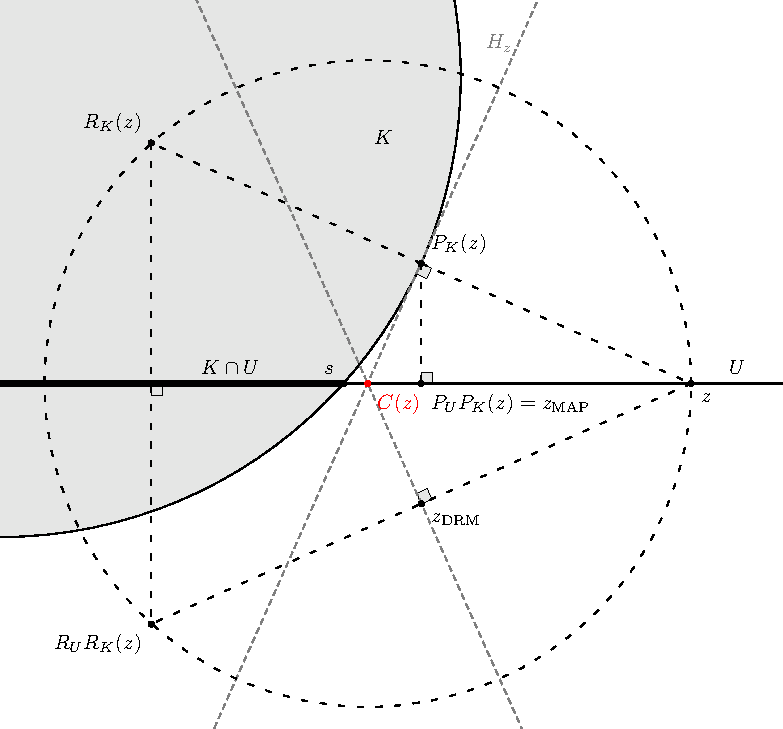
\includegraphics[scale=0.8]{ConvexAffine}
	\caption{Illustration of CRM, MAP and DRM for the intersection between an affine U and a convex K.}
	\label{fig:CRM MAP DRM comp}
\end{figure}

\begin{fact}[Comparing CRM, MAP and DRM]
Assume $K, U \subset \RR^{n}$ as in \cref{fact:CRM well def char} and let $z \in U$ be given. Also recall the notation $z_{\mathrm{MAP}}:=P_{U} P_{K}(z), z_{\mathrm{DRM}}:=\frac{1}{2}\left(\mathrm{Id}+R_{U} R_{K}\right)(z)$ and $C(z):=\operatorname{circumcenter}\left\{z, R_{K}(z), R_{U} R_{K}(z)\right\}$
Then, for any $s \in K \cap U$ we have
\begin{listi}
	\item $\|C(z)-s\| \leq\left\|z_{\mathrm{MAP}}-s\right\| \leq\left\|z_{\mathrm{DRM}}-s\right\|$,
	\item $\dist(C(z), K \cap U) \leq \dist\left(z_{\mathrm{MAP}}, K \cap U\right) \leq \dist\left(z_{\mathrm{DRM}}, K \cap U\right)$.
\end{listi}
\end{fact}
\begin{proof}
	See the proof for Theorem 2 in \cite{Behling:2020}.
\end{proof}

A similar comparison will be made for the approximate variants of CRM and MAP only, as no suitable DRM equivalent exists.

Before we present CARM, we first need to discuss what we mean by approximate projections and why the particular definition we use for CARM was chosen instead of other existing approximations for orthogonal projections.

\newpage
\section{Approximate projections}\label{sec:approx proj}

We recall that the main objective of this work is to adapt an existing projection method by employing approximate projections in place of the exact (orthogonal) projections. For this purpose, one of the many proposed methods of approximating projections had to be chosen. 
Each of them relinquishes or modifies certain properties of the orthogonal projections, in order to circumvent the unavailability of said projections or to avoid problems derived from some of these properties. These projections have been given names such as \emph{approximate}, \emph{inexact} or \emph{relaxed}, with some inconsistencies as to the use of these adjectives.

First, we present the definition of approximate projection chosen for our work.

\subsection{Outer-approximate projections}
The notion of an \emph{outer-approximate projection} was introduced by Fukushima in~\cite[Lemma 4]{Fukushima:1983}, whose definition we present below. In subsequent sections, we will use the terms outer-approximate projection and approximate projection interchangeably. 
\begin{definition}[Outer-approximate projector]\label{def:approx proj}
	Let $B \subseteq \RR^{n}$ be a nonempty set and $X \subseteq \RR^{n}$ a closed and convex set. A function $\tilde{P}_{X}: B \rightarrow \RR^{n}$ is called an \emph{outer-approximate projector} defined on $B$ and associated to $X$ if the following properties are satisfied
	\begin{listi}
		\item there exists $\gamma \in [0,1)$ such that
		\begin{equation}
			\dist\left(\tilde{P}_{X}(x), X\right) \leq \gamma \dist(x, X), \text { for all } x \in B;
		\end{equation}
		\item  for any $x \in B,$ it holds that
		\begin{equation}
			\scal{x-\tilde{P}_{X}(x)}{y-\tilde{P}_{X}(x)} \leq 0, \text { for all } y \in X.
		\end{equation}
	\end{listi}
\end{definition}

The point $\tilde{P}_{X}(x)$ will be called \emph{outer-approximate projection} of $x \in B$ onto $X$. \cref{def:approx proj} guarantees, in view of property (ii), the existence of a hyperplane $H_{X}(x)$ separating $x$ from $X$ such that $\tilde{P}_{X}(x)$ is the orthogonal projection of $x$ onto $H_{X}(x)$. In light of this, we can interpret property (i) as meaning that the distance of the hyperplane $H_{X}(x)$ to $X$ is at least a fixed percentage of the distance from $x$ to $X$. This percentage is given by $\gamma$; if $\gamma=0$, the outer-approximate projection is precisely the exact orthogonal projection. If, for instance, $\gamma = 0.3$, then $\tilde{P}_{X}(x)$ advances at least $70 \%$ towards $X$ by means of the distance of $x$ to $X$. We emphasize that a percentage of improvement on the distance, \emph{per se}, is not sufficient for having an outer-approximate projection; the existence of the separating hyperplane is crucial, too.

In short, it can be said that the outer-approximate projection preserves the sense of approaching the target set from the "outside" (like a relaxed projection, as we will discuss later), that is, by means of a hyperplane separating the original point being projected and the set it is being projected towards, as well as establishing a minimum gain in distance relative to the original point, keeping the idea that a projection should bring a point somewhat closer to the target set, whenever the point does not belong to the set. Unfortunately, this approach sacrifices the nonexpansivity of the projection and it does not require the approximate projection to lie on the target set.

Now, we will present alternative definitions of "approximate" (in a general sense) projections and comment briefly on how they differ from the one we chose to employ.

\subsection{Alternative definitions of approximate projections}

The following two definitions were taken from \cite{Drusvyatskiy:2018}. This paper also attempts to avoid the intractability of exact projections, (mostly focusing on nonconvex sets, however). Instead of providing a method for finding a more computational-friendly approximate projection, Drusvyatskyi and Lewis allow, to a certain degree, errors on the computation of the exact projections, still obtaining convergence of an alternating projections scheme with non-exact projections onto one of the sets.

The first approximation was named by the authors as an \emph{inexact} projection, in the sense that it establishes a bound for computing errors in the calculation of the projection whilst not imposing further conditions.

\begin{definition}[Drusvyatskyi and Lewis' inexact projection]
	Let $B \subseteq \RR^{n}$ be a nonempty set and $X \subseteq \RR^{n}$ a closed set. For some $\varepsilon \geq 0$, $\tilde{P}_{X}(x)$ is a DL-inexact projection from $x \in B$ onto $X$ if $\|\tilde{P}_{X}(x)-P_{X}(x)\| \leq \varepsilon \dist(x,X)$.
\end{definition}

This definition allows for employing of a slightly miscalculated projection. It assumes the exact projection is known, but that its exact computation might be inefficient or erroneous to a certain extent. Thus, it is not suitable for replacing projections when they are unknown or unavailable.

The second definition, presented below, was called an \emph{approximate} projection. While similar in intent to the inexact projection, this approximation is now required to be on the target set.

\begin{definition}[Drusvyatskyi and Lewis' approximate projection]
	Let $B \subseteq \RR^{n}$ and $X \subseteq \RR^{n}$ be closed sets. Let $z \in X$ and $y \in B$ such that $y \in P_{B}(z)$. For some $\varepsilon \geq 0$, $\tilde{P}_{X}(y)$ is an approximate projection of $y$ onto $X$ if  $\|\tilde{P}_{X}(y)-P_{X}(y)\| \leq \varepsilon \|y - z\|$.
\end{definition}

In \cite{Goncalves:2019}, Gonçalves, Gonçalves and Oliveira propose a variation on the Levenberg-Marquardt method using a type of feasible inexact projection which they call an $\varepsilon$-projection. These projections can be obtained iteratively, using the conditional gradient (Frank-Wolfe) method \cite{Frank:1956, Jaggi:2013}, and can replace exact projections when costly or unavailable. In that sense, they work more similarly to Fukushima's outer-approximate projections than either of Drusvyatskyi and Lewis' projections. The definition of the (inexact) $\varepsilon$-projection is given below.

\begin{definition}[$\varepsilon$-projection]\label{def:epsilon-projection}
	Let $K$ be a nonempty closed convex set contained in an open set $\Omega \subset \RR^n$. Let $x \in \RR^{n}$ and $\varepsilon \geq 0$ be given. $P_{K}(x, \varepsilon)$ is an \emph{$\varepsilon$-projection} of $x$ onto $K$ when
	\[
	P_{K}(x, \varepsilon) \in K \text{ and } \scal{x-P_{K}(x, \varepsilon)}{y-P_{K}(x, \varepsilon)} \leq \varepsilon, \text{ for all } y \in K.
	\]
\end{definition}
The $\varepsilon$-projection has some interesting properties. Not only does the $\varepsilon$-projection lie on the target set, we also have that the orthogonal projection is recovered if $\varepsilon=0$. In this characterization, the variational inequality of the projection theorem is only approximated and not preserved, as with the outer-approximate projection; however, this approximation on the inequality, combined with the fact that $P_{K}(x, \varepsilon) \in K$, allows for a pseudo-nonexpansivity of the operator $P_{K}(\cdot,\cdot)$ which we will refer to as the $\varepsilon$-nonexpansivity property.

\begin{fact}[$\varepsilon$-nonexpansivity]
	For any $x, y \in \RR^{n}$ and $\varepsilon \geq 0$, we have
	$$
	\left\|P_{K}(x, \varepsilon)-P_{K}(y)\right\| \leq\|x-y\|+\sqrt{\varepsilon}
	$$
\end{fact}
\begin{proof}
	It follows from \cref{fact:proj thm} and \cref{def:epsilon-projection} that
	$$
	\left\langle x-P_{K}(x), P_{K}(x, \varepsilon)-P_{K}(x)\right\rangle \leq 0, \quad\left\langle x-P_{K}(x, \varepsilon), P_{K}(x)-P_{K}(x, \varepsilon)\right\rangle \leq \varepsilon,
	$$
	which combined yield
	$$
	\left\langle x-P_{K}(x)-x+P_{K}(x, \varepsilon), P_{K}(x, \varepsilon)-P_{K}(x)\right\rangle \leq \varepsilon
	$$
	or, equivalently,
	$$
	\left\|P_{K}(x)-P_{K}(x, \varepsilon)\right\| \leq \sqrt{\varepsilon}.
	$$
	Therefore, using the triangle inequality and \cref{fact:proj nonexp}, we have
	\[
	\left\|P_{K}(x, \varepsilon)-P_{K}(y)\right\| \leq\left\|P_{K}(x, \varepsilon)-P_{K}(x)\right\|+\left\|P_{K}(x)-P_{K}(y)\right\| \leq \sqrt{\varepsilon}+\|x-y\|.
	\]
\end{proof}

Finally, we discuss \emph{relaxed projections}, which are the averages of a point and its projection.

\begin{definition}[Relaxed projection]\label{def:relax proj}
	Let $A$ be a nonempty closed subset of $\RR^n$, $x \in \RR^n$ and $\lambda \in (0,1)$. $\hat{P}_{A}(x; \lambda)$ is a $\lambda$-relaxed projection of $x$ on $A$ if 
	$$
	\hat{P}_{A}(x; \lambda)=(1-\lambda)x+\lambda P_{A}(x).
	$$
\end{definition}
One could also present a similar definition with $\lambda \in [0,1]$, in which case we would have that $\hat{P}_{A}(x;1)=P_{A}(x)$ and $\hat{P}_{A}(x;0)=x$.
The notion of relaxed projection can also be expanded to accept $\lambda \in (1,2)$, in which case the relaxed projections are averages of the projection and its associated reflection. In this extended definition, relaxed projections with $\lambda \in (0,1)$ are called \emph{underrelaxed projections}, while those associated with $\lambda \in (1,2)$ are called \emph{overrelaxed projections}. With this in mind, unless stated otherwise, by relaxed projections we mean underrelaxed projections (as defined in \cref{def:relax proj}).

Unlike the outer-approximate and $\varepsilon$-projections, which can replace exact projections when they are unavailable, relaxed projections rely on the existence of exact projections to be determined, thus being unfit for this role. Their main utility comes when replacing exact projections in situations where convergence may be faster or larger regions of convergence can be obtained from not taking a full projection step, such as in the Method of Alternating Relaxed Projections (MARP) \cite{Bauschke:2013}, which employs a scheme similar to MAP's, though replacing the exact projections with relaxed ones.

Relaxed projections can also be seen as a special case of an outer-approximate projection, as proved below.

\begin{proposition}[Relaxed projection is an outer-approximate projection]
	Let $B \subseteq \RR^n$ be a nonempty set and let $X \subseteq \RR^n$ be a closed convex set. Let $x \in B$, $\lambda \in (0,1)$ and $\hat{P}_{X}(x; \lambda)$ be as defined in \cref{def:relax proj}. Then $\hat{P}_{X}(x; \lambda)$ is an outer-approximate projection, as defined in \cref{def:approx proj}.
\end{proposition}
\begin{proof}
	First, let's prove that $\hat{P}_{X}(x;\lambda)$ satisfies \cref{def:approx proj}(i). Using the triangular inequality and the fact that $P_{X}(x) \in X$, we have that
	\begin{align}
			\dist(\hat{P}_{X}(x;\lambda),X) &\leq \|\hat{P}_{X}(x;\lambda)-P_{X}(x)\| + \dist(P_{X}(x),X) \\
			&= \|(1-\lambda)x+\lambda P_{X}(x)-P_{X}(x)\| \\
			&= (1-\lambda)\|x-P_{X}(x)\|,
	\end{align}
	which implies that
	\[
	\dist(\hat{P}_{X}(x;\lambda),X) \leq (1-\lambda)\dist(x,X).
	\]
	Since $(1-\lambda) \in (0,1)$, letting $\gamma=1-\lambda$ establishes (i) is satisfied.
	
	To prove \cref{def:approx proj}(ii), from \cref{def:relax proj} and \cref{fact:proj thm}, we have 
	\begin{align}
		\scal{x-\hat{P}(x;\lambda)}{y-\hat{P}(x;\lambda)}
		&=\scal{\lambda x - \lambda P_{X}(x)}{y - (1-\lambda)x -\lambda P_{X}(x)} \\
		&=\lambda\scal{x-P_{X}(x)}{y-P_{X}(x)} \\
		&\quad+\lambda\scal{x-P_{X}(x)}{-(1-\lambda)x+(1-\lambda)P_{X}(x)} \\
		&=\lambda\underbrace{\scal{x-P_{X}(x)}{y-P_{X}(x)}}_{\leq 0}+\underbrace{\lambda(\lambda-1)}_{<0}\|x-P_{X}(x)\|^2 \leq 0,		
	\end{align}
	thus proving (ii) is satisfied.
	
	Since (i) and (ii) are satisfied, the statement is proved.
\end{proof}

While these alternative definitions are interesting and useful in the adequate contexts, the properties and the existence of an algorithm for their computation made the outer-approximate projections the more well-suited approximation for our intended objective.

In the next section, we introduce our main algorithm, which modifies CRM \cref{subsec:CRM} by employing outer-approximate projections (and reflections) onto the convex set in a product space environment, while the projections and reflections onto the affine subspace (which have closed form) remain exact.

\newpage
\section{Circumcentered Approximate Projection Method - CARM}\label{sec:CARM}
In this section, we  define the Circumcentered-Approximate Reflection Method (CARM) and show that it solves CFP-red \cref{eq:KcapU}, that is,
\[
\text{ find } z^{*}\in K\cap U, 
\]
with $K \subset \RR^{n}$ a closed convex set, $U \subset \RR^{n}$ an affine subspace and $K \cap U \neq \emptyset$.

Let us assume that an outer-approximate projector $\tilde{P}_{K}$ onto $K$ is available. According to \cref{def:approx proj}, we have a fixed scalar $\gamma \in [0,1)$  and a set $B\subset \RR^{n}$. We will consider $B$ as $\RR^{n}$. Thus,  the correspondent \emph{outer-approximate reflection} $\tilde{R}_{K}: \RR^{n} \rightarrow \RR^{n}$ is given by $\tilde{R}_{K}=2 \tilde{P}_{K}-\Id$.

CARM initializes in $U$ and along its iterates employs outer-approximate reflections through $K$ and exact reflections through $U$. In fact, CARM iterates as
$$
z^{k+1}=\tilde{C}\left(z^{k}\right)\coloneqq \circum\left\{z^{k}, \tilde{R}_{K}\left(z^{k}\right), R_{U} \tilde{R}_{K}\left(z^{k}\right)\right\}, \text { with } z^{k} \in U.
$$
Recall that the circumcenter $\tilde{C}(z^{k})$ is the point equidistant to $z^{k}, \tilde{R}_{K}\left(z^{k}\right)$ and  $R_{U} \tilde{R}_{K}\left(z^{k}\right)$ lying in $\aff\{z^{k}, \tilde{R}_{K}\left(z^{k}\right), R_{U} \tilde{R}_{K}\left(z^{k}\right)\}$; see \cref{def:circum}. We refer to $\tilde{C}(\cdot)$ as the \emph{outer-approximate circumcenter operator}. The consistency of the iteration above will be proved in the sense that, when $z^{0}\in U$, the sequence is well-defined and remains in $U$. 

Connections between CARM and CRM make this section's structure similar to \cite[Section 2]{Behling:2020}, though the outer-approximate projections and reflections have to be carefully incorporated in the new analysis; indeed, CRM is a special case of CARM when the outer-approximate projections employed are the exact orthogonal projections (that is, when $\gamma = 0$).

Our first results concern the well-definedness of the outer-approximate circumcenter operator in $U$ and the characterization of the domain. We are going to see that \[U \subset \operatorname{dom}(\tilde{C})\coloneqq \left\{z \in \RR^{n} \mid \tilde{C}(z)=\circum \left\{z, \tilde{R}_{K}(z), R_{U}\tilde{R}_{K}(z)\right\}\right\}\] and $\tilde{C}(z) \in U,$ whenever $z \in U$.

\begin{lemma}[Well-definedness and characterization of the CARM iteration] \label{lem:CARM well-def char} 
	Let $K, U \subset \RR^{n}$, where $K$ is a closed convex set and $U$ is an affine subspace and assume $K \cap U \not = \emptyset$. Then, for all $z \in U$, the CARM iteration $\tilde{C}(z)\coloneqq \circum\left\{z, \tilde{R}_{K}(z), R_{U}\tilde{R}_{K}(z)\right\}$ is well-defined and we have $\tilde{C}(z) \in U$. Furthermore, $\tilde{C}(z)=P_{\tilde{H}_{z} \cap U}(z)$,
	where $\tilde{H}_{z}\coloneqq \left\{x \in \RR^{n} \mid \scal{x-\tilde{P}_{K}(z)}{z-\tilde{P}_{K}(z)}=0\right\}$ if $z \notin K$ and $\tilde{H}_{z}\coloneqq K$, otherwise.
\end{lemma}
	\begin{proof}
    %On the proof for Lemma 3 in \cite[Section 2]{Behling:2020}, simply replace $C_{z}$ with $\tilde{C}_{z}$ and the hyperplane $H_{z}$ with $\tilde{H}_{z}$. The proof follows similarly, since we can derive from the outer-approximate projection a hyperplane separating $z$ from $K$, albeit further from $K$ than the hyperplane derived from the exact projection.

	Let $z \in U$. If $z \in K$, the result is trivial. Suppose then that $z \in U \setminus K$. From the definition of $\tilde{H}_{z}$, we can clearly see that  $P_{\tilde{H}_{z}}(z)=\tilde{P}_{K}(z)$ and, consequently, $R_{\tilde{H}_{z}}(z)=\tilde{R}_{K}(z)$. Note that $\tilde{H}_{z} \cap U \neq \emptyset$.
	
	Let $y \in K \cap U$.
	$y \in K$ and \cref{def:approx proj}(ii) imply $\scal{z-\tilde{P}_{K}(z)}{y-\tilde{P}_{K}(z)} \leq 0$.
	Define $f:[0,1] \rightarrow \RR$ by $f(t)\coloneqq \scal{z-\tilde{P}_{K}(z)}{tz+(1-t) y-\tilde{P}_{K}(z)}$.
	Then 
	\begin{align}
			f(0)&=\scal{z-\tilde{P}_{K}(z)}{y-\tilde{P}_{K}(z)} \leq 0, \text{ and}\\
			f(1)&=\scal{z-\tilde{P}_{K}(z)}{z-\tilde{P}_{K}(z)}=\left\|z-\tilde{P}_{K}(z)\right\|^{2}>0.
	\end{align}
	Since $f$ is continuous, there exists a scalar $\bar{t} \in[0,1)$ such that
	\[
	f(\bar{t})=\scal{z-\tilde{P}_{K}(z)}{\bar{t} z+(1-\bar{t}) y-\tilde{P}_{K}(z)}=0,
	\]
	implying $\bar{t} z+(1-\bar{t}) y \in \tilde{H}_{z}$.
	
	On the other hand, since $U$ is an affine subspace and $z, y \in U$, we have $\bar{t}z+(1-\bar{t})y \in U$ as well.
	Altogether, $\bar{t} z+(1-\bar{t}) y \in \tilde{H}_{z} \cap U$.
	Therefore, \[\tilde{C}(z)=\circum\left\{z, \tilde{R}_{K}(z), R_{U}\tilde{R}_{K}(z)\right\}=\circum\left\{z, R_{\tilde{H}_{z}}(z), R_{U}R_{\tilde{H}_{z}}(z)\right\}=P_{\tilde{H}_{z} \cap U}(z),\] where
	the last equality follows by employing  \cref{fact:CRM 1 step conv hp aff}.
\end{proof}

Next, we characterize the fixed point set of the outer-approximate circumcenter operator, as well as the fixed point sets of the outer-approximate projectors and reflectors.
\begin{lemma}[Fixed points of $\tilde{P}_{K}, \tilde{R}_{K}$ and $\tilde{C}$]\label{lem:CARM fix} 
	Assume $K, U \subset \RR^{n}$ as in  \cref{lem:CARM well-def char} and consider $\Fix \tilde{P}_{K}\coloneqq \{z \in \RR^{n} \mid \tilde{P}_{K}(z)=z\}$, $\Fix \tilde{R}_{K}\coloneqq \{z \in \RR^{n} \mid \tilde{R}_{K}(z)=z\}$ and $\Fix \tilde{C}\coloneqq \{z \in \operatorname{dom}(\tilde{C}) \mid \tilde{C}(z)=z\}$. Then,
	\begin{listi}
	\item $\Fix \tilde{P}_{K}=\Fix \tilde{R}_{K}=K$; 
	\item $\Fix \tilde{C}=K \cap U$.
	\end{listi}
\end{lemma}
	\begin{proof}
	\begin{listi}
	\item Note that $z=\tilde{R}_{K}(z) = 2\tilde{P}_{K}(z)-z$ implies that $z=\tilde{P}_{K}(z)$. Therefore, $\Fix \tilde{P}_{K}=\Fix \tilde{R}_{K}$. 
	Clearly, if $z \in K$ then $z \in\Fix \tilde{P}_{K}$. Conversely, take $z \in \Fix \tilde{P}_{K}$, i.e., $\tilde{P}_{K}(z)=z$.
    By \cref{def:approx proj}(i), we have that $\operatorname{dist}(\tilde{P}_{k}(z), K) \leq \gamma \operatorname{dist}(z, K)$, where $\gamma \in [0,1)$. If $\gamma=0$, then $z=\tilde{P}_{K}(z)=P_{K}(z)$ and $z \in K$ trivially. Otherwise, if $\gamma \in (0,1)$, from $z = \tilde{P}_{K}(z)$ it follows that $\operatorname{dist}(z, K) \leq \gamma \operatorname{dist}(z, K)$. This is only true if $\operatorname{dist}(z, K)=0$, which means that $z \in K$. Therefore, that $\Fix \tilde{P}_{K}=K$.
	\item It is easy to see that, if $z \in K \cap U$ then $z \in \Fix \tilde{R}_{K} \cap \Fix R_{U}$ and thus $z \in \Fix \tilde{C}$. On the other hand, take $z \in \Fix \tilde{C}$. By the definition of $\tilde{C}(z)$, we have that $\tilde{C}(z)=z$ implies $z=\tilde{R}_{K}(z)=R_{U}\tilde{R}_{K}(z)$. Since $\Fix \tilde{R}_{K}=K$ by (i), $z=\tilde{R}_{K}(z)$ implies $z \in K$. Then, $z=R_{U}(z)$, which yields that $z \in U$. Therefore, $z \in K \cap U$.
	\end{listi}
\end{proof}

Note that the outer-approximate projection parameter $\gamma$ being strictly less than $1$ in \cref{def:approx proj} is key to deriving the previous result.

We now derive the firm quasinonexpansiveness property (\cref{def:nonexp}(iv)) of the outer-approximate circumcenter operator $\tilde{C}$ restricted to $U$.
\begin{lemma}[CARM is firmly quasinonexpansive] \label{lem:CARM quasinonexp}
	Assume $K, U \subset \RR^{n}$ as in  \cref{lem:CARM well-def char}. Then, for any $z \in U$ and $s \in K \cap U$
	\begin{equation}\label{eq: CARM fqne}
		\|\tilde{C}(z)-s\|^{2} \leq \|z-s\|^{2}-\|z-\tilde{C}(z)\|^{2}.
		\end{equation}
	Moreover,
	\begin{equation}
		\dist^{2}(\tilde{C}(z), K \cap U) \leq \dist^{2}(z, K \cap U)-\|z-\tilde{C}(z)\|^{2}.
	\end{equation}
\end{lemma}
	\begin{proof}
	%On the proof of Lemma 5 \cite[Section 2]{Behling:2020}, replace exact projections and reflections onto/through $K$ with outer-approximate ones and replace the corresponding hyperplanes with $\tilde{H}_{z}\coloneqq \left\{h \in \RR^{n} \mid \scal{h-\tilde{P}_{K}(z)}{z-\tilde{P}_{K}(z)}=0\right\}$ and \\ $\tilde{H}_{z}^{+}\coloneqq \left\{h \in \RR^{n} \mid \scal{h-\tilde{P}_{K}(z)}{z-\tilde{P}_{K}(z)}\leq\right.0\}$.
	
	
	Let $z \in U$. Define $\tilde{H}_{z} \coloneqq \left\{h \in \RR^{n} \mid \scal{h-\tilde{P}_{K}(z)}{z-\tilde{P}_{K}(z)}=0\right\}$ and $\tilde{H}_{z}^{+} \coloneqq \left\{h \in \RR^{n} \mid \scal{h-\tilde{P}_{K}(z)}{z-\tilde{P}_{K}(z)}\leq\right.0\}$. Clearly, $K \subseteq \tilde{H}_{z}^{+}$, thus $K \cap U \subseteq \tilde{H}_{z}^{+} \cap U$. If $z \in \tilde{H}_{z}$, then $z \in K \cap U$ and, by  \cref{lem:CARM fix}(ii), $\tilde{C}(z)=z$, from which the result easily follows.
	
	Let $z \notin \tilde{H}_{z}$. Since $\tilde{R}_{K}(z)=R_{\tilde{H}_{z}}(z)$,  $\tilde{C}(z)=\circum\left\{z, R_{\tilde{H}_{z}}(z), R_{U}R_{\tilde{H}_{z}}(z)\right\}$. From  \cref{fact:CRM 1 step conv hp aff}, we have that $\tilde{C}(z)=P_{\tilde{H}_{z}\cap U}(z) \in U$. Note that $z \not\in \tilde{H}_{z}$ implies that $z \not\in K$. It also easily follows that $z \notin \tilde{H}_{z}^{+}$, which combined with the fact that $\tilde{H}_{z}$ is the boundary of $\tilde{H}_{z}^{+}$ yield that $P_{\tilde{H}_{z} \cap U}(z)=P_{\tilde{H}_{z}^{+} \cap U}(z)$.
	
	Considering that for any $s \in K \cap U, P_{\tilde{H}_{z}^{+} \cap U}(s)=s$, we have
	\begin{align}
	\|\tilde{C}(z)-s\|^{2}& =\left\|P_{\tilde{H}_{z} \cap U}(z)-s\right\|^{2} \\
		&=\left\|P_{\tilde{H}_{z}^{+} \cap U}(z)-P_{\tilde{H}_{z}^{+} \cap U}(s)\right\|^{2} \\
		&\leq\|z-s\|^{2}-\left\|\left[z-P_{\tilde{H}_{z}^{+} \cap U}(z)\right]-\left[s-P_{\tilde{H}_{z}^{+} \cap U}(s)\right]\right\|^{2} \\
		&=\|z-s\|^{2}-\|z-\tilde{C}(z)\|^{2},
	\end{align}
	where we use the firm nonexpansiveness of the projection (\cref{fact:proj nonexp}) to obtain the inequality.
	
	Finally, plug $P_{K \cap U}(z)$ in for $s$ in \cref{eq: CARM fqne} so as to get
	\begin{align}
		\dist^{2}(\tilde{C}(z), K \cap U) & \leq\|\tilde{C}(z)-P_{K \cap U}(z)\|^{2} \leq\|z-P_{K \cap U}(z)\|^{2}-\|z-\tilde{C}(z)\|^{2} \\
		&=\dist^{2}(z, K \cap U)-\|z-\tilde{C}(z)\|^{2}.
	\end{align}
	Then, $\tilde{C}$ is firmly quasinonexpansive.
\end{proof}

We can now establish the central theorem of this work, stating convergence of CARM. Although the proof follows some lines of \cite[Theorem 1]{Behling:2020}, one has to be careful when dealing with the fixed points of the outer-approximate reflection operator $\tilde{R}_{K}$. In this regard, \cref{lem:CARM fix} plays a special role.

\begin{theorem}[Convergence of CARM]\label{thm:CARM conv}
	Assume $K, U \subset R^{n}$ as in Lemma 2 and let $z \in U$ be given. Then, the CARM sequence $\left(\tilde{C}^{k}(z)\right)_{k \in \NN}$ is well-defined, contained in $U$ and converges to a point in $K \cap U$.
\end{theorem}
\begin{proof}
	 \cref{lem:CARM well-def char} gives us that $\left(\tilde{C}^{k}(z)\right)_{k \in \NN}$ is well-defined and belongs to $U$. From  \cref{lem:CARM quasinonexp}, we have, for any $z \in U, s \in K \cap U$ and $\ell \in \NN$
	\begin{align}
		\left\|z^{\ell+1}-s\right\|^{2} &=\left\|\tilde{C}^{\ell+1}(z)-s\right\|^{2} \\
		&=\left\|\tilde{C}\left(\tilde{C}^{\ell}(z)\right)-s\right\|^{2} \\
		& \leq\left\|\tilde{C}^{\ell}(z)-s\right\|^{2}-\left\|\tilde{C}^{\ell}(z)-\tilde{C}\left(\tilde{C}^{\ell}(z)\right)\right\|^{2} \\
		&=\left\|\tilde{C}^{\ell}(z)-s\right\|^{2}-\left\|\tilde{C}^{\ell}(z)-\tilde{C}^{\ell+1}(z)\right\|^{2} \\
		&=\left\|z^{\ell}-s\right\|^{2}-\left\|z^{\ell}-z^{\ell+1}\right\|^{2}.
	\end{align}
	Hence, for all $\ell \in \NN$
	\begin{align}
		\left\|z^{\ell}-z^{\ell+1}\right\|^{2} \leq\left\|z^{\ell}-s\right\|^{2}-\left\|z^{\ell+1}-s\right\|^{2}.
	\end{align} 
	Summing from $\ell=0$ to $m$, we have
	\begin{equation}
		\sum_{\ell=0}^{m}\left\|z^{\ell}-z^{\ell+1}\right\|^{2} \leq \sum_{\ell=0}^{m}\left(\left\|z^{\ell}-s\right\|^{2}-\left\|z^{\ell+1}-s\right\|^{2}\right)=\left\|z^{0}-s\right\|^{2}-\left\|z^{m+1}-s\right\|^{2} \leq\left\|z^{0}-s\right\|^{2}.
	\end{equation}
	Taking limits as $m \rightarrow+\infty$, we get the summability of the associated series and so, 	
	\begin{equation}\label{eq:CARM conv eq 1}
		\|z^{k}-z^{k+1}\| \rightarrow 0 \text{ as } k \rightarrow+\infty.
	\end{equation}
	Moreover, by \cref{eq: CARM fqne} in  \cref{lem:CARM quasinonexp}, the sequence $\left(z^{k}\right)_{k \in \NN}$ is bounded. That is,
	\begin{equation}
		\left\|z^{k}-s\right\| = \left\|\tilde{C}^{k}(z)-s\right\| \leq\left\|\tilde{C}^{k-1}(z)-s\right\| \leq \cdots \leq\|z-s\|.
	\end{equation}
	This also shows that the sequence is Fejér monotone with respect to $K \cap U$.
	
	Let $\hat{z}$ be any cluster point of the sequence $\left(z^{k}\right)_{k \in \NN}$ and denote $\left(z^{i_{k}}\right)_{k \in \NN}$ an associated convergent subsequence to $\hat{z}$. Note further that the fact $z^{i_{k}}-z^{i_{k}+1} \rightarrow 0$ implies $z^{i_{k}+1} \rightarrow \hat{z}$. We claim that $\hat{z} \in K \cap U$. Since $U$ is closed and $\left(z^{k}\right)_{k \in \NN}$ is contained in $U$, we must have $\hat{z} \in U$. 
	
	From \cref{def:approx proj}(i), for any $z^{k}$ we have that
	\begin{align}			
		\dist(z^{k},K)&=\left\|P_{K}(z^{k})-z^{k}\right\|\\
		&\leq\left\|\tilde{P}_{K}\left(z^{k}\right)-z^{k}\right\|+\dist\left(\tilde{P}_{K}\left(z^{k}\right),K\right)\\
		&\leq\left\|\tilde{P}_{K}\left(z^{k}\right)-z^{k}\right\|+\gamma\dist(z^{k},K) \\
		&\leq \frac{1}{1-\gamma}\left\|\tilde{P}_{K}\left(z^{k}\right)-z^{k}\right\|,
	\end{align}
	with $\gamma \in [0,1)$.
	Therefore, $$
	\left\|\tilde{P}_{K}\left(z^{k}\right)-z^{k}\right\| \geq (1-\gamma) \dist(z^{k},K)\geq 0.
	$$
	
	Let $z^{i^{k}} \in U$ such that $z^{i^{k}} \rightarrow \hat{z}$.
	Assume by contradiction that $\rho = \dist(\hat{z},K)>0$. Then, we have that 
	$$
	\left\|\tilde{P}_{K}\left(\hat{z}\right)-\hat{z}\right\| \geq (1-\gamma) \dist(\hat{z},K)=(1-\gamma)\rho >0.
	$$
	From the definitions of $\tilde{P}, \tilde{R}$ and $\tilde{C}$, for any $i^k$ we have
	\begin{align}
		\left\|\tilde{P}_{K}(z^{i^{k}})-z^{i^{k}}\right\|&=\left\|\frac{z^{i^{k}}+\tilde{R}(z^{i^{k}})}{2}-z^{i^{k}}\right\|=\frac{1}{2}\left\|\tilde{R}_{K}(z^{i^{k}})-z^{i^{k}}\right\|\\
		&\leq\frac{1}{2}\left(\left\|\tilde{R}_{K}(z^{i^{k}})-\tilde{C}(z^{i^{k}})\right\|+\left\|\tilde{C}(z^{i^{k}})-z^{i^{k}}\right\| \right)\\
		&=\left\|\tilde{C}(z^{i^{k}})-z^{i^{k}}\right\|.
	\end{align}
	 Hence, we have that
	 \begin{equation}\label{eq:CARM conv eq 2}	 		 \|z^{i^{k+1}}-z^{i^{k}}\|=\|\tilde{C}(z^{i^{k}})-z^{i^{k}}\| \geq \left\|\tilde{P}_{K}\left(z^{i^{k}}\right)-z^{i^{k}}\right\| \geq (1-\gamma) \dist(z^{i^{k}},K). 
	 \end{equation}
	Also, note that
	$$
	\rho \leq \|\hat{z}-P_{K}(z^{i^k})\| \leq \|\hat{z}-z^{i^{k}}\|+\|z^{i^{k}}-P_{K}(z^{i^{k}})\| =\|\hat{z}-z^{i^{k}}\|+\dist(z^{i^{k}},K).
	$$

	Since $z^{i^{k}} \rightarrow \hat{z}$, for all $i^{k}$ sufficiently large we must have $\|z^{i^{k}}-\hat{z}\|\leq \frac{\rho}{2}$. Then, taking into account the previous inequality, we have that $\dist(z^{i^{k}},K)\geq \frac{\rho}{2}$ for all sufficiently large $i^{k}$, which combined with \cref{eq:CARM conv eq 2} yields
	$$
	\|z^{i^{k+1}}-z^{i^{k}}\|\geq (1-\gamma) \dist(z^{i^{k}},K) \geq (1-\gamma)\frac{\rho}{2}.
	$$
	However, this prevents $\|z^{i^{k+1}}-z^{i^{k}}\| \rightarrow 0$ as $i^{k} \rightarrow \infty$, contradicting \cref{eq:CARM conv eq 1}.
	Thus, $\hat{z} \in K$.
	
	%So, $z^{i k+1}-\tilde{R}_{K}\left(z^{i k}\right)$ converges to $0$. Then, taking limits as $k \rightarrow+\infty$ in the last equality, we have that $\hat{z}=\tilde{R}_{K}(\hat{z})$; that is, $\hat{z} \in \Fix \tilde{R}_{K}$. From \cref{lem:CARM fix}(i), $\hat{z} \in K$, proving the claim.
	Finally, we have that $\left(z^{k}\right)_{k \in \NN}$ is bounded, contained in $U$, Fejér monotone with respect to $K \cap U$  and all its cluster points are in $K \cap U$. Applying \cref{fact:Fejer conv thm} establishes the desired result.
\end{proof}

\subsection{CARM for general convex intersection}

Now, we'll show that CARM can be used for finding a point in the intersection of finitely many closed convex sets using Pierra's product space reformulation \cite{Pierra:1984hl}. Consider CFP-red \cref{eq:KcapU}, that is,
\[
\text{ find } z^{*}\in K\cap U, 
\]
where $K=K_{1} \times K_{2} \times \cdots \times K_{m}\subset \RR^{nm}$ is the Cartesian product of $m$ closed and convex sets $K_{i} \in \RR^n$ and $U :=\left\{(x, x, \ldots, x) \in \RR^{nm} \mid x \in \RR^{n}\right\}$ is the diagonal set, which can be easily shown to be a subspace of $\RR^{nm}$.

Considering $m$ arbitrary vectors $x^{(i)}$ in $\RR^{n},$ with $i=1, \ldots, m$, we can build an arbitrary point $z=\left(x^{(1)}, x^{(2)}, \ldots, x^{(m)}\right) \in \RR^{nm}$. The projection onto $U$ is given by
\begin{equation}
P_{U}(z)=\frac{1}{m}\left(\sum_{i=1}^{m} x^{(i)}, \sum_{i=1}^{m} x^{(i)}, \ldots, \sum_{i=1}^{m} x^{(i)}\right).
\end{equation}
\label{Pierra P_{U}}

The following proposition establishes an outer-approximate projection for $K$, following the properties given in \cref{def:approx proj}.

\begin{proposition}[Outer-approximate projection on product space]\label{prop:prod space approx proj}
Assume $K$ and $U$ as above. Let $z=\left(x^{(1)}, x^{(2)}, \ldots, x^{(m)}\right) \in \RR^{nm}$ be an arbitrary point in $\RR^{nm}$ given by $m$ arbitrary vectors $x^{(i)} \in K_{i} \subset \RR^{n}$. For each set $K_{i}$, let $\tilde{P}_{K_{i}}$ be an approximate projector associated with the parameter $\gamma_{i} \in [0,1)$ as per \cref{def:approx proj}(i) and let $\gamma_{\max}\coloneqq\max \{\gamma_{1}, \ldots, \gamma_{m}\}$. Then,
\begin{align}\label{eq:PierraP_K}
\tilde{P}_{K}(z)=(\tilde{P}_{K_{1}}  (x^{(1)}), \ldots, \tilde{P}_{K_{m}}(x^{(m)}))    
\end{align}
is an outer-approximate projection that satisfies \cref{def:approx proj} with the associated parameter $\gamma_{\max}$.
\end{proposition}

\begin{proof}
    \begin{listi}
    \item Note that, from the definition of distance and \cref{def:approx proj}(i), we have
    \begin{align}
        \dist^{2}(\tilde{P}_{K}(z), K)
        &= \sum_{i=1}^{m} \dist^{2}(\tilde{P}_{K_{i}}(x^{(i)}), K_{i}) \\
        &\leq \sum_{i=1}^{m} \gamma_{i}^{2}\dist^{2}(x^{(i)}, K_{i}) \\
        &\leq \gamma_{max}^{2} \sum_{i=1}^{m}\dist^{2}(x^{(i)}, K_{i}) = \gamma_{max}^{2} \dist^{2}(z,K),       
    \end{align}
    Thus, we have that $\dist(\tilde{P}_{K}(z), K) \leq \gamma_{max} \dist(z,K)$, satisfying property (i).
    \item Let $y=(y^{(1)},\ldots,y^{(m)}) \in \RR^{nm}$ be an arbitrary point in $\RR^{nm}$, where $y^{(i)} \in K_{i} \subset \RR^{n}$. Following the definition of inner product, we have that
    \begin{align}
        \scal{z-\tilde{P}_{K}(z)}{y-\tilde{P}_{K}(z)}
        = \sum_{i=1}^{m} \scal{x^{\left(i\right)}-\tilde{P}_{K}\left(x^{\left(i\right)}\right)}{y^{\left(i\right)}-\tilde{P}_{K}\left(x^{\left(i\right)}\right)}\leq 0,
    \end{align}
    in which we use the fact that, by \cref{def:approx proj}(ii), the $m$ terms of the sum are lesser or equal than 0. Thus, property (ii) is also satisfied.
    \end{listi}
\end{proof}

Following this proposition, we can establish convergence of CARM for general convex intersection.

\begin{theorem}[Convergence of CARM for general convex intersection]\label{thm:CARM conv general}
Assume $K, U \subset \RR^{n}$ as above and let $x^{0} \in \RR^{n}$ be given. Then, taking as initial point $z^{0}:=\left(x^{0}, x^{0}, \ldots, x^{0}\right) \in U$, we have that the sequence $\left\{z^{k}\right\} \subset \RR^{nm}$ generated by
\[
z^{k+1}:=\circum\left\{z^{k}, \tilde{R}_{K}\left(z^{k}\right), R_{U}\tilde{R}_{K}\left(z^{k}\right)\right\}
\]
is well defined, entirely contained in $U$ and converges to a point $z^{*}=\left(x^{*}, x^{*}, \ldots, x^{*}\right) \in \RR^{nm}$, where $x^{*} \in \bigcap_{i=1}^{m} K_{i}$.
\end{theorem}
\begin{proof}
The result follows immediately from \cref{thm:CARM conv}, with $\tilde{R}_{K}$ being given by $\tilde{P}_{K}$ as defined in \cref{prop:prod space approx proj}.
\end{proof}

We have come to the favorable conclusion that CARM converges to a solution of \cref{eq:KcapU} when initializing in $U$, which generalizes Theorems 1 and 3 from \cite{Behling:2020}. Following this line of generalizing results from \cite{Behling:2020}, we now look at alternating projections employing outer-approximate projections onto one of the sets. 



\newpage
\section{Approximate Method of Alternating Projections - AMAP}\label{sec:AMAP}
In this section, the problem under consideration is given by
$$
\text { Find } z^{*} \in K_1 \cap K_2
$$
with $K_1, K_2$ being closed convex sets and $K_1 \cap K_2 \not = \emptyset$. We will assume that exact projections are available for $K_2$, but not for $K_1$. Of course, this problem is more general than CFP-red \cref{eq:KcapU}, since a subspace $U$ of $\RR^{n}$ is closed and convex. 

We are going to establish convergence of AMAP for finding a point in the intersection of the two closed convex sets $K_1$ and $K_2$. We understand that such a result can be derived from known frameworks for inexact alternating projections; nonetheless, we present it for the sake of completeness. Other approximation techniques concerning MAP can be found, for instance, in \cite{Luke:2012, Luke:2013}.

We will initialize AMAP on $K_{2}$ and replace MAP's orthogonal projections onto $K_1$ by outer-approximate ones. Let us describe AMAP formally. For a given point $z \in \RR^{n}$, we generate a sequence $\left(x^{k}\right)_{k \in \NN}$ contained in $K_{2}$ such that $x^{0} \coloneqq P_{K_{2}}(z)$ and
$$
x^{k+1}=P_{K_{2}}\tilde{P}_{K_{1}}\left(x^{k}\right), \quad k=0,1,2, \ldots
$$

MAP is a special case of AMAP and we are able to carry out a convergence analysis for AMAP resembling MAP's. 

We note that our intention is to provide an alternative for CARM in its intended setting (CFP-red where projections onto $K$ are unavailable), in which case $K$ will play the role of $K_1$ and $U$ will play the role of $K_2$. However, in the proofs that follow, we can see that the convex set for which projections are available does need not be an affine subspace for AMAP to converge.

One could develop an even more general version of AMAP, in which outer-approximate projections are employed for both convex sets. However, this would require extra effort and ultimately would not be more useful for our intended application. Expanding AMAP for a setting in which neither one of the sets has projections available is left as a suggestion for further work.

We will start our analysis with a Fejér monotonicity statement.

\begin{proposition}[Fejér monotonicity of AMAP sequence]\label{prop:AMAP Fejer}
	Suppose $K_{1},K_{2} \subseteq \RR^{n}$ are closed convex sets and $K_{1} \cap K_{2} \neq \emptyset$. Let $x^{0} \in K_{2}$ be any point in $K_{2}$. Then the sequences $\left(x^{k}\right)_{k \in \NN}$ and $\left(\tilde{P}_{K_{1}}\left(x^{k}\right)\right)_{k \in \NN}$ generated by the AMAP algorithm is Fejér monotone with respect to $K_{1} \cap K_{2}$.
\end{proposition}
\begin{proof}
	Let $\bar{x}$ be any point in the intersection $K_{1} \cap K_{2}$, and let $k \in \NN$. We have that
	\begin{align}
		\left\|x^{k}-\bar{x}\right\|^{2} &=\left\|x^{k}-\tilde{P}_{K_1}(x^k)+\tilde{P}_{K_1}(x^k)-\bar{x}\right\|^{2} \\
		&=\left\|x^{k}-\tilde{P}_{K_1}(x^k)\right\|^{2}+\left\|\tilde{P}_{K_1}(x^k)-\bar{x}\right\|^{2}+2\scal{x^{k}-\tilde{P}_{K_1}(x^k)}{\tilde{P}_{K_1}(x^k)-\bar{x}} \\
		& \geq\left\|x^{k}-\tilde{P}_{K_1}(x^k)\right\|^{2}+\left\|\tilde{P}_{K_1}(x^k)-\bar{x}\right\|^{2}
	\end{align}
	where $-\scal{x^{k}-\tilde{P}_{K_1}(x^k)}{\tilde{P}_{K_1}(x^k)-\bar{x}}=\scal{x^{k}-\tilde{P}_{K_1}(x^k)}{\bar{x}-\tilde{P}_{K_1}(x^k)} \leq 0$ from \cref{def:approx proj}(ii). Thus, we have that
	\begin{equation}\label{eq:AMAP fejer 1}
		\left\|\tilde{P}_{K_{1}}\left(x^{k}\right)-\bar{x}\right\|^{2} \leq \left\|x^{k}-\bar{x}\right\|^{2} - \left\|x^{k}-\tilde{P}_{K_{1}}\left(x^{k}\right)\right\|^{2} \leq \left\|x^{k}-\bar{x}\right\|^{2}.
	\end{equation}
	Similarly, we also have that
	\begin{equation}\label{eq:AMAP fejer 2}
		\left\|x^{k+1}-\bar{x}\right\|^{2} \leq \left\|\tilde{P}_{K_{1}}\left(x^{k}\right)-\bar{x}\right\|^{2} - \left\|\tilde{P}_{K_{1}}\left(x^{k}\right)-x^{k+1}\right\|^{2} \leq \left\|\tilde{P}_{K_{1}}\left(x^{k}\right)-\bar{x}\right\|^{2}.
	\end{equation}
	From \cref{eq:AMAP fejer 1,eq:AMAP fejer 2}, it follows that $\left\|x^{k+1}-\bar{x}\right\| \leq \left\|x^{k}-\bar{x}\right\|$
	and $\left\|\tilde{P}_{K_{1}}\left(x^{k+1}\right)-\bar{x}\right\| \leq \left\|\tilde{P}_{K_{1}}\left(x^{k}\right)-\bar{x}\right\|$.

	Since $k$ and $\bar{x}$ are arbitrary, the sequences $\left(x^{k}\right)_{k \in \NN}$ and $\left(\tilde{P}_{K_{1}}\left(x^{k}\right)\right)_{k \in \NN}$ are Fejér monotone with respect to $K_1 \cap K_2$.
\end{proof}

The following proposition establishes the domain of the set of the cluster points of the sequence generated by AMAP.
\begin{proposition}[AMAP cluster points]\label{prop:AMAP cluster}
	Suppose $K_{1},K_{2} \subseteq \RR^{n}$ are closed convex sets and $K_{1} \cap K_{2} \neq \emptyset$. Let $x^{0} \in K_{2}$ be any point in $K_{2}$. Then every cluster point of the sequence $\left(x^{k}\right)_{k \in \NN}$ generated by the AMAP algorithm belongs to $K_{1} \cap K_{2}$.
\end{proposition}
	\begin{proof}
	Since the sequence $\left(x^{k}\right)_{k \in \NN}$ is Fejér monotone with respect to $K_{1} \cap K_{2}$, it is bounded. Therefore, it must have at least one cluster point.
	
	Let $x^{*}$ be a cluster point for the sequence $\left(x^{k}\right)_{k \in \NN}$. Since $K_{2}$ is closed, and $x^{k} \in K_{2}$ for all $k \in \NN$, then $x^{*} \in K_{2}$.
	
	Rearranging \cref{eq:AMAP fejer 1,eq:AMAP fejer 2}, we have that
	\begin{align}
	\left\|\tilde{P}_{K_{1}}\left(x^{k}\right)-x^{k}\right\| \leq  \left\|x^{k}-\bar{x}\right\|^{2} - \left\|\tilde{P}_{K_{1}}\left(x^{k}\right)-\bar{x}\right\|^{2} \label{eq:AMAP fejer 3} \text{, and} \\
	\left\|x^{k+1}-\tilde{P}_{K_{1}}\left(x^{k}\right)\right\| \leq \left\|\tilde{P}_{K_{1}}\left(x^{k}\right)-\bar{x}\right\|^{2} - \left\|x^{k+1}-\bar{x}\right\|^{2}. \label{eq:AMAP fejer 4}
	\end{align}
	From \cref{eq:AMAP fejer 1,eq:AMAP fejer 2}, we find that the sequence
	$$
	\left\|x^{0}-\bar{x}\right\|,\left\|\tilde{P}_{K_{1}}\left(x^{0}\right)-\bar{x}\right\|,\left\|x^{1}-\bar{x}\right\|,\left\|\tilde{P}_{K_{1}}\left(x^{1}\right)-\bar{x}\right\|, \ldots
	$$
	is decreasing; thus, it converges. Therefore, taking the limit on  \cref{eq:AMAP fejer 3,eq:AMAP fejer 4} yields that $\left\|\tilde{P}_{K_{1}}\left(x^{k}\right)-x^{k}\right\|$ and $\left\|x^{k+1}-\tilde{P}_{K_{1}}\left(x^{k}\right)\right\|$ converge to zero.
	
	From \cref{def:approx proj}(i), we have that
	\begin{align}			
		\dist(x^{k},K_{1})&=\left\|P_{K_{1}}(x^{k})-x^{k}\right\|\\
		&\leq\left\|\tilde{P}_{K_{1}}\left(x^{k}\right)-x^{k}\right\|+\dist\left(\tilde{P}_{K_{1}}\left(x^{k}\right),K_{1}\right)\\
		&\leq\left\|\tilde{P}_{K_{1}}\left(x^{k}\right)-x^{k}\right\|+\gamma\dist(x^{k},K_{1}) \\
		&\leq \frac{1}{1-\gamma}\left\|\tilde{P}_{K_{1}}\left(x^{k}\right)-x^{k}\right\|, 
	\end{align}
where $\gamma \in [0,1)$ is the outer-approximate projection parameter associated to $K_{1}$. From the fact that $\left\|\tilde{P}_{K_{1}}\left(x^{k}\right)-x^{k}\right\| \rightarrow 0$, we must have that $\dist(x^{k},K_{1}) \rightarrow 0$.

Since a subsequence of $(x_k)_{k\in\NN}$ converges to $x^{*}$ and $\dist(x^{k},K_{1}) \rightarrow 0$, $x^{*}$ must be a cluster point of $K_{1}$. Thus, $x^{*} \in K_{1}$, since $K_{1}$ is closed and therefore must contain all of its cluster points. Hence,  we conclude that $x^{*} \in K_{1} \cap K_{2}$. 
\end{proof}

%It's important to note here that $\gamma$ is a constant and $\gamma \in [0,1)$. Suppose instead we have a sequence $\left(\gamma_{k}\right)_{k \in \NN}$ where $\gamma_{k} \in [0,1)$. In that case, we could have a sequence in which $\gamma_{k} \rightarrow 1$ ``faster'' than $\left\|y^{k}-x^{k}\right\| \rightarrow 0$, such that $\dist(x^{k},K_{2}) \not \rightarrow 0$. However, since $\gamma \in [0,1)$ is constant, no matter how ``slowly'' $\left\|y^{k}-x^{k}\right\| \rightarrow 0$, we have that $\dist(x^{k},K_{2}) \rightarrow 0$.

Following the previous results, we can establish our main convergence result for AMAP.

\begin{theorem}[AMAP convergence]\label{thm:AMAP conv} 
	Suppose $K_{1},K_{2} \subseteq \RR^{n}$ are closed convex sets and $K_{1} \cap K_{2} \neq \emptyset$. Let $x^{0} \in K_{2}$ be any point in $K_{2}$. Then the sequence $\left(x^{k}\right)_{k \in \NN}$ generated by the AMAP algorithm converge to a point $x^{*} \in K_{1} \cap K_{2}$.
\end{theorem}
\begin{proof}
	From \cref{prop:AMAP Fejer,prop:AMAP cluster}, we have that $\left(x^{k}\right)_{k \in \NN}$ is Fejér monotone with respect to $K_{1} \cap K_{2}$ and that every cluster point of $\left(x^{k}\right)_{k \in \NN}$ belongs to $K_{1} \cap K_{2}$. The result follows from applying \cref{fact:Fejer conv thm}.
\end{proof}

%Still in this paper, we are going to investigate CARM's rate of convergence under a regularity assumption, referred to as error bound condition.



\newpage
\section{Comparing CARM and AMAP}\label{sec:comp}
In this section, we compare CARM and AMAP for finding a point in the intersection of a closed convex set $K$ and an affine subspace $U$, both belonging to $\RR^{n}$. Our study is divided in two subsections. In the first, we show that for a point in the affine set, the CARM iteration is always closer to the solution set than the AMAP iteration. In the second subsection, the methods are compared under an error bound assumption. The error bound guarantees that both CARM and AMAP achieve linear convergence, with CARM having a better asymptotic rate than AMAP.

\subsection{Myopic comparison}\label{subsec:myopic comp}

We look at CARM and AMAP acting on an arbitrary point $z$ in the affine set $U$. As previously done for CRM and MAP in \cref{subsubsec:CRM for CFP}, we will present a similar figure to illustrate how CARM and AMAP compare in a geometrical sense. In this figure, we also feature the point generated by CRM, in order to establish a reference to that method as well. We recall that $C$ is the CRM operator and $\tilde{C}$ is the CARM operator.

\begin{figure}[h!]
	\centering
	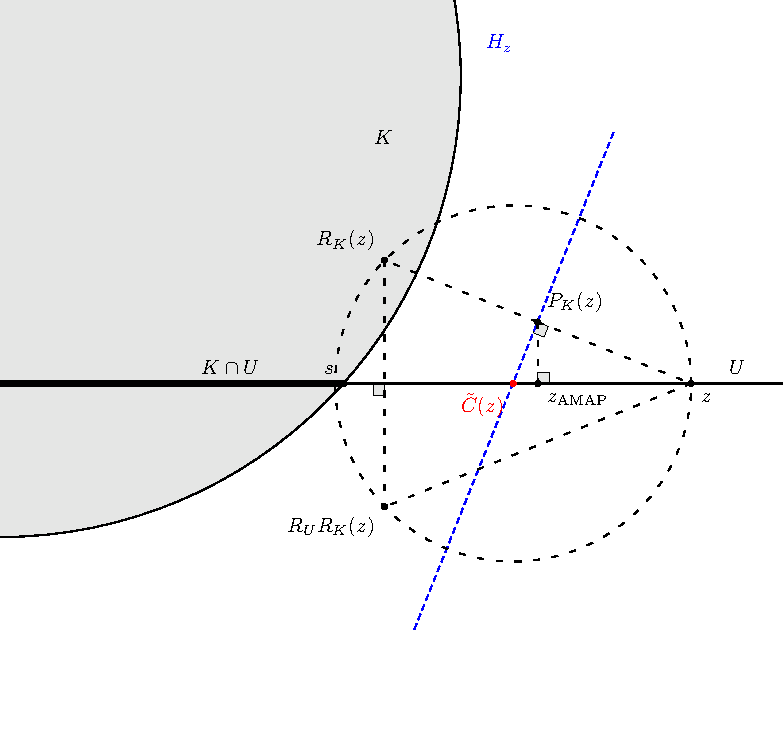
\includegraphics[scale=0.8]{ConvexAffine-CARM}
	\caption{Illustration of CARM and AMAP for the intersection between an affine U and a convex K.}
	\label{fig:CARM AMAP comp}
\end{figure}

We prove that CARM brings you closer to $K \cap U$ than AMAP. This result generalizes \cite[Theorem 2]{Behling:2020} and is stated formally in the following theorem. We note that DRM lacks an equivalent outer-approximation based variant; by replacing the projection onto $K$ with an outer-approximate one, we are no longer assured that the sequence will remain in $U$ and, consequently, that it will converge to $K \cap U$. Thus, we only consider CARM and AMAP in this comparison.

\begin{theorem}[CARM versus AMAP]\label{thm:CARM x AMAP} Assume $K, U \subset \RR^{n}$ are as in  \cref{lem:CARM well-def char} and let $z \in U$ be given. Also recall the notation $z_{\mathrm{\AMAP}}\coloneqq P_{U}\tilde{P}_{K}(z)$ and $\tilde{C}(z)\coloneqq \circum \left\{z, \tilde{R}_{K}(z), R_{U} \tilde{R}_{K}(z)\right\}$.
	Then, for any $s \in K \cap U$ we have
	\begin{listi}
		\item $\|\tilde{C}(z)-s\| \leq\left\|z_{\AMAP}-s\right\|$;
		\item $\dist(\tilde{C}(z), K \cap U) \leq \dist\left(z_{\mathrm{\AMAP}}, K \cap U\right)$.
	\end{listi}
\end{theorem}
\begin{proof}
	Assume $z \in U$ and let $s \in K \cap U$ be arbitrary but fixed. If $z \in K$ the result follows trivially, because then $P_{U} \tilde{P}_{K}(z)=z$, $\frac{1}{2}\left(\Id+R_{U} \tilde{R}_{K}\right)(z)=z$ and $\tilde{C}(z)=z$ due to  \cref{lem:CARM fix}. So, let $z \in U \backslash K$. From  \cref{lem:CARM well-def char}, we have that $\tilde{C}(z)$ is the projection of $z$ onto the intersection of $U$ and the hyperplane with normal $z-\tilde{P}_{K}(z)$ passing through $\tilde{P}_{K}(z)$. Therefore, the triangles $\triangle{[z, \tilde{P}_{K}(z), \tilde{C}(z)]}$ and $\triangle{[z, P_{U}\tilde{P}_{K}(z), \tilde{P}_{K}(z)]}$ have right angles $\angle{[z, \tilde{P}_{K}(z), \tilde{C}(z)]}$ and $\angle{[z,P_{U}\tilde{P}_{K}(z), \tilde{P}_{K}(z)]}$ (the latter since $U$ is a subspace), respectively. Hence,
	\begin{equation}\label{eq:myopic 1}
		\|\tilde{C}(z)-z\| \geq\left\|\tilde{P}_{K}(z)-z\right\| \geq\left\|P_{U}\tilde{P}_{K}(z)-z\right\|.	\end{equation}
	Now, note that $P_{U}\tilde{P}_{K}(z)$, $z$ and $\tilde{C}(z)$ are collinear, since both $P_{U} \tilde{P}_{K}(z)$ and $\tilde{C}(z)$ lie in the semi-line starting at $z$ and passing through $P_{U}\tilde{R}_{K}(z)=\frac{1}{2}\left(\tilde{R}_{K}(z)+R_{U}\tilde{R}_{K}(z)\right)$. In fact, this semi-line contains the circumcenter $\tilde{C}(z)$ as it is a bisector of the isosceles triangle $\triangle{[z, \tilde{R}_{K}(z),R_{U}\tilde{R}_{K}(z)]}$. Since $P_{U}$ is a linear operator \cref{fact:aff proj} $z \in U$, we have that
	\begin{align}
		z_{\mathrm{\AMAP}} &=P_{U} \tilde{P}_{K}(z)=P_{U}\left(\frac{1}{2}\left(z+\tilde{R}_{K}(z)\right)\right)=\frac{1}{2} P_{U}\left(z+\tilde{R}_{K}(z)\right) \\
		&=\frac{1}{2}\left(P_{U}(z)+P_{U} \tilde{R}_{K}(z)\right)=\frac{1}{2}\left(z+P_{U} \tilde{R}_{K}(z)\right)
	\end{align}
	Thus, $z_{\AMAP}$ is a convex combination of $z$ and $P_{U}\tilde{R}_{K}(z)$ with parameter $\frac{1}{2}$. Therefore, we have more than just collinearity of $z, \tilde{C}(z)$ and $z_{\AMAP}$. Both $\tilde{C}(z)$ and $z_{\AMAP}$ lie on the semi-line starting at $z$ and passing through $P_{U}\tilde{R}_{K}(z)$. This means that $z$ cannot lie between $\tilde{C}(z)$ and $z_{\AMAP}$ and, in view of \cref{eq:myopic 1}, the only remaining possibility is that $z_{\AMAP}$ is a convex combination of $\tilde{C}(z)$ and $z$, that is, there exists a parameter $r \in[0,1]$ such that
	\begin{equation}
		z_{\AMAP}=r\tilde{C}(z)+(1-r)z
	\end{equation}
	and
	\begin{equation}
		z_{\AMAP}-\tilde{C}(z)=(1-r)(z-\tilde{C}(z)) \text { and } z-z_{\AMAP}=r(z-\tilde{C}(z)).
	\end{equation}
	$r$ must be strictly larger than zero;  otherwise $z$ would be in $K \cap U$. Thus,
	\begin{equation}\label{eq:myopic 2}
		z_{\AMAP}-C(z)=\frac{1-r}{r}\left(z-z_{\AMAP}\right)
	\end{equation}
	This equation will be properly combined with the following inner product manipulations
	\begin{align}
		\scal{z-z_{\AMAP}}{\tilde{C}(z)-s}=&\scal{z-\tilde{P}_{K}(z)}{\tilde{C}(z)-s}+\scal{\tilde{P}_{K}(z)-z_{\AMAP}}{\tilde{C}(z)-s} \notag \\
		=&\scal{z-\tilde{P}_{K}(z)}{\tilde{C}(z)-\tilde{P}_{K}(z)}+\underbrace{\scal{z-\tilde{P}_{K}(z)}{\tilde{P}_{K}(z)-s}}_{\geq 0} \notag \\
		&+\underbrace{\scal{\tilde{P}_{K}(z)-z_{\AMAP}}{\tilde{C}(z)-s)}}_{=0}  \\
		\geq 0\label{eq:myopic 3}
	\end{align}
	The first under-brace equality follows as a consequence of the property outlined in \Cref{def:approx proj}(ii). The last under-brace remark holds since $\tilde{P}_{K}(z)-z_{\AMAP}$ is orthogonal to the subspace $U$ and both $\tilde{C}(z)$ and $s$ are in $U $. Now, inequality \cref{eq:myopic 3} together with equation \cref{eq:myopic 2} give us
	\begin{equation}
		\scal{z_{\AMAP}-C(z)}{s-C(z)}=\frac{1-r}{r}\scal{z-z_{\AMAP}}{s-C(z)} \leq 0
	\end{equation}
	which, due to the cosine rule, leads to $\|\tilde{C}(z)-s\| \leq\|z_{\AMAP}-s\|$ for any $s \in K \cap U$. Taking this into account and letting $\hat{z}, \tilde{z} \in K \cap U$ realize the distance of $\tilde{C}(z), z_{\AMAP}$ to $K \cap U$, respectively, we have
	\begin{equation}
		\dist(\tilde{C}(z), K \cap U)=\|\tilde{C}(z)-\hat{z}\| \leq\|\tilde{C}(z)-\tilde{z}\| \leq\|z_{\AMAP}-\tilde{z}\|=\dist(z _{\AMAP}, K \cap U)	
	\end{equation}
	proving the first inequalities in items (i) and (ii).
\end{proof}

\subsection{CARM and AMAP under error bound}\label{subsec:comp EB}
Now, inspired by the results in \cite{Arefidamghani:2020}, we show that CARM achieves better convergence rates than AMAP under an error bound assumption (EB). We are going to prove that the EB condition, defined below, ensures linear convergence of the sequences $\left(z^{k}\right)_{k \in \NN}$ and $\left(x^{k}\right)_{k \in \NN}$ generated by AMAP and CARM, respectively.

\begin{assumption}[Error bound condition]\label{eb}
Let $K \subset \RR^{n}$ be a closed and convex set  and $U \subset \RR^{n}$ an affine subspace. Assume that $K \cap U \neq \emptyset$ and there exists $\omega \in(0,1)$ such that $\dist(x, K) \geq \omega \dist\left(x, K \cap U\right)$ for all $x \in U$ and $\dist(y, U) \geq \omega \dist\left(y, K \cap U\right)$ for all $y \in K$.
\end{assumption}

To begin our convergence analysis, a corollary of the following proposition will prove that, for both methods, the sequences $\left(\dist\left(z^{k}, K \cap U\right)\right)_{k \in \NN}$ and $\left(\dist\left(x^{k}, K \cap U\right)\right)_{k \in \NN}$ both converge linearly to $0$. For the following passages, recall that $\gamma \in [0,1)$.

\begin{proposition}\label{prop:EB dist}
	Assume that $K, U$ satisfy EB. Consider $\tilde{T}, \tilde{C}: \RR^{n} \rightarrow \RR^{n}$ as in $\tilde{T}=P_{U} \circ \tilde{P}_{K},$ $\tilde{C}(\cdot)=\circum\left(\cdot, \tilde{R}_{K}(\cdot), R_{U}\left(\tilde{R}_{K}(\cdot)\right)\right)$. Then, for all $x \in U$,
	\begin{equation}\label{eq:dist KcapU AMAP CARM}
		\left(1-\omega^{2}(1-\gamma)^2\right) \dist^{2}(x, K \cap U) \geq \dist^{2}(\tilde{T}(x), K \cap U) \geq \dist^{2}(\tilde{C}(x), K \cap U)
	\end{equation}
	with $\omega$ as in Assumption EB.
\end{proposition}
\begin{proof}
    Note that
	\begin{align}
		\|\tilde{T}(x)-P_{K \cap U}(x)\|^{2} &=\left\|P_{U}\left(\tilde{P}_{K}(x)\right)-P_{K \cap U}(x)\right\|^{2} \\
		&\leq \left\|\tilde{P}_{K}(x)-P_{K \cap U}(x)\right\|^{2}-\left\|P_{U}\left(\tilde{P}_{K}(x)\right)-\tilde{P}_{K}(x)\right\|^{2} \\ &\leq\left\|\tilde{P}_{K}(x)-P_{K \cap U}(x)\right\|^{2} \leq\|x-P_{K \cap U}(x)\|^{2}-\left\|x-\tilde{P}_{K}(x)\right\|^{2} \\
		&\leq \|x-P_{K \cap U}(x)\|^{2}-(1-\gamma)^2\dist^{2}(x, K) \\ &\leq (1-\omega^{2}(1-\gamma)^{2}) \dist^{2}(x, K \cap U) \label{eq:dist AMAP x KcapU}
	\end{align}
	for all $x \in U$,  where we use the firm quasinonexpansivity of the projection onto $U$ (\cref{def:nonexp}(iv)) and the fact that $P_{K \cap U} \in U$ to obtain the first inequality; the
	firm quasinonexpansivity of the outer-approximate projection onto $K$ (which can easily be derived from \cref{def:approx proj}(ii)), the fact that $P_{K \cap U} \in K$, and  $K = \Fix \tilde{P}_{K}$ from \cref{lem:CARM fix}(i) give us the third inequality; finally, we employ \cref{def:approx proj}(i) and Assumption EB to obtain the last two inequalities. From \cref{eq:dist AMAP x KcapU} and the definition of $P_{K \cap U}$, we get
	\begin{align}
		\left\|\tilde{C}(x)-P_{K \cap U}(\tilde{C}(x))\right\|^{2} & \leq\left\|\tilde{C}(x)-P_{K \cap U}(\tilde{T}(x))\right\|^{2}  \\
		& \leq\left\|\tilde{T}(x)-P_{K \cap U}(\tilde{T}(x))\right\|^{2} \leq\left\|\tilde{T}(x)-P_{K \cap U}(x)\right\|^{2}  \\
		&=\left(1-\omega^{2}(1-\gamma)^{2}\right)\left\|x-P_{K \cap U}(x)\right\|^{2},\label{eq:dist CARM x KcapU}
	\end{align}
	using \cref{thm:CARM x AMAP}(i) in the second inequality.  \cref{eq:dist KcapU AMAP CARM}follows immediately from \cref{eq:dist AMAP x KcapU} and \cref{eq:dist CARM x KcapU}, after rewriting the appropriate terms in terms of distance, in view of the definition of $\tilde{P}_{K \cap U}$.
	\end{proof}
With the corollary below, we can establish an upper bound for the asymptotic constants of Q-linear convergence for both CARM and AMAP.
\begin{corollary}[Upper bound for asymptotic constants of CARM and AMAP under EB]\label{prop:EB Q conv}
	Let $\left(z^{k}\right)_{k \in \NN}$ and $\left(x^{k}\right)_{k \in \NN}$ be the sequences generated by AMAP and CARM starting at any $z^{0} \in U$ and any $x^{0} \in \RR^{n}$, respectively. If $K, U$ satisfy Assumption EB then the sequences $\left(\dist\left(z^{k}, K \cap U\right)\right)_{k \in \NN}$ and $\left(\dist\left(x^{k}, K \cap U\right)\right)_{k \in \NN}$ converge Q-linearly to $0$, and the asymptotic constants are bounded above by $\sqrt{1-\omega^{2}(1-\gamma)^{2}}$, with $\omega$ as in Assumption EB.
\end{corollary}
\begin{proof}
    Since $\left(z^{k}\right)_{k \in \NN} \subset U$ and $z^{k+1}=T\left(z^{k}\right)$, from the first inequality in \cref{eq:dist KcapU AMAP CARM} we get
	\begin{align}
		\left(1-\omega^{2}(1-\gamma)^{2}\right) \dist^{2}\left(z^{k}, K \cap U\right) \geq \dist^{2}\left(z^{k+1}, K \cap U\right),
	\end{align}
    from which we obtain, assuming $z^k \notin K \cap U$,
	\begin{align}\label{eq: AMAP upper bound}
		\frac{\dist\left(z^{k+1}, K \cap U\right)}{\dist\left(z^{k}, K \cap U\right)} \leq \sqrt{1-\omega^{2}(1-\gamma)^{2}}.
	\end{align}
	Considering the second inequality in \cref{eq:dist KcapU AMAP CARM}, following the same steps gives us
	\begin{align}\label{eq: CARM upper bound 1}
		\frac{\dist\left(x^{k+1}, K \cap U\right)}{\dist\left(x^{k}, K \cap U\right)} \leq \sqrt{1-\omega^{2}(1-\gamma)^{2}},
	\end{align}
	in which we also assume that $x^k \notin K\cap U$.
	The inequalities in \cref{eq: AMAP upper bound,eq: CARM upper bound 1} imply the result.
\end{proof}
We remark that the result for AMAP still holds when $U$ is any closed and convex set, but for  CARM we need $U$ to be an affine subspace, as it might diverge otherwise.

We'll now show that, under Assumption EB, CARM achieves a linear rate with an asymptotic constant better than the one given in \cref{prop:EB Q conv}.
\begin{proposition}[Improved upper bound for asymptotic constant of CARM under EB]\label{prop:CARM linear rate}
	Let $\left(x^{k}\right)_{k \in \NN}$ be the sequence generated by CARM starting at any $x^{0} \in \RR^{n}$. If $K, U$ satisfy Assumption EB then the sequence $\left(\dist\left(x^{k}, K \cap U\right)\right)_{k \in \NN}$ converges to 0 with the asymptotic constant bounded above by $\sqrt{\frac{1-\omega^{2}(1-\gamma)^2}{1+\omega^{2}(1-\gamma)^2}},$ where $\omega$ is as in Assumption EB.
\end{proposition}
\begin{proof}
	Take $y^{*} \in K \cap U$ and $x \in U$. Note that
	\begin{align}
		\dist^{2}(x, K) &=\left\|x-P_{K}(x)\right\|^{2}\leq \frac{1}{(1-\gamma)^2}\left\|x-\tilde{P}_{K}(x)\right\|^{2}  \\
		& \leq\frac{1}{(1-\gamma)^2}\left(\left\|x-y^{*}\right\|^{2}-\left\|\tilde{P}_{K}(x)-y^{*}\right\|^{2}\right) \\
		&=\frac{1}{(1-\gamma)^2}\left(\left\|x-y^{*}\right\|^{2}-\left\|\tilde{P}_{K}(x)-\tilde{P}_{K}\left(y^{*}\right)\right\|^{2}\right)  \\
		& \leq\frac{1}{(1-\gamma)^2}\left(\left\|x-y^{*}\right\|^{2}-\left\|P_{U}\left(\tilde{P}_{K}(x)\right)-P_{U}\left(\tilde{P}_{K}\left(y^{*}\right)\right)\right\|^{2}\right.\\
		&\quad\left.-\left\|P_{U}\left(\tilde{P}_{K}(x)\right)-\tilde{P}_{K}(x)\right\|^{2}\right)  \\
		&=\frac{1}{(1-\gamma)^2}\left(\left\|x-y^{*}\right\|^{2}-\left\|P_{U}\left(\tilde{P}_{K}(x)\right)-y^{*}\right\|^{2}-\left\|P_{U}\left(\tilde{P}_{K}(x)\right)-\tilde{P}_{K}(x)\right\|^{2}\right)\label{eq: dist^2(xK)}
	\end{align}
	using the firm quasinonexpansiveness of the outer-approximate projection and the fact that $y^{*} \in K$ in second inequality, and the firm nonexpansiviness of the orthogonal projection onto $U$ in the last inequality.
	
	From \cref{lem:CARM well-def char}, we have that $\tilde{C}(x)=P_{\tilde{H}_{x} \cap U}(x)$ with
	\[
	\tilde{H}_{x}\coloneqq \left\{y \in \RR^{n} \mid\left\langle y-\tilde{P}_{K}(x), x-\tilde{P}_{K}(x)\right\rangle \leq 0\right\} \supset K.
	\]
	Hence,
	$\left\langle y^{*}-\tilde{C}(x), x-\tilde{C}(x)\right\rangle \leq 0$ and since $x, P_{U}\left(\tilde{P}_{K}(x)\right)$ and $\tilde{C}(x)$ are collinear by \cref{eq:myopic 2}, we get $\left\langle y^{*}-\tilde{C}(x), P_{U}\left(\tilde{P}_{K}(x)\right)-\tilde{C}(x)\right\rangle \leq 0$. Thus,
	\begin{equation}\label{eq: dist AMAP CARM col}
		\left\|P_{U}\left(\tilde{P}_{K}(x)\right)-y^{*}\right\|^{2} \geq\left\|\tilde{C}(x)-y^{*}\right\|^{2}+\left\|\tilde{C}(x)-P_{U}\left(\tilde{P}_{K}(x)\right)\right\|^{2}.
	\end{equation}
	Now, \cref{eq: dist AMAP CARM col,eq: dist^2(xK)} imply
	\begin{align}
		\dist^{2}(x, K) & \leq\frac{1}{(1-\gamma)^2}\left(\left\|x-y^{*}\right\|^{2}-\left\|\tilde{C}(x)-y^{*}\right\|^{2}-\left\|\tilde{C}(x)-P_{U}\left(\tilde{P}_{K}(x)\right)\right\|^{2}\right. \\
		&\left.-\left\|P_{U}\left(\tilde{P}_{K}(x)\right)-\tilde{P}_{K}(x)\right\|^{2}\right) \\
		&=\frac{1}{(1-\gamma)^2}\left(\left\|x-y^{*}\right\|^{2}-\left\|\tilde{C}(x)-y^{*}\right\|^{2}-\left\|\tilde{C}(x)-\tilde{P}_{K}(x)\right\|^{2}\right) \\
		& \leq\frac{1}{(1-\gamma)^2}\left(\left\|x-y^{*}\right\|^{2}-\left\|\tilde{C}(x)-y^{*}\right\|^{2}-\dist^{2}(\tilde{C}(x), K)\right) \\
		& \leq\frac{1}{(1-\gamma)^2}\left(\left\|x-y^{*}\right\|^{2}-\dist^{2}(\tilde{C}(x), K \cap U)-\dist^{2}(\tilde{C}(x), K)\right)
	\end{align}
	using the definition of the distance in the last two inequalities. Now, taking $y^{*}=P_{K \cap U}(x)$ and using the error bound condition for $x$ and $C(x),$ we obtain
	\begin{align}
		\omega^{2}\dist^{2}(x, K \cap U) &\leq \frac{1}{(1-\gamma)^2}\dist^{2}(x, K) \\
		&\leq \frac{1}{(1-\gamma)^2}\left(\dist^{2}(x, K \cap U)-\dist^{2}(\tilde{C}(x), K \cap U)\right.\\
		&\quad\left.- \omega^{2}(1-\gamma)^{2} \dist^{2}(\tilde{C}(x), K \cap U)\right)  \\
		&=\frac{1}{(1-\gamma)^2}\dist^{2}(x, K \cap U)\\
		&\quad-\frac{1}{(1-\gamma)^2}\left(1+\omega^{2}(1-\gamma)^{2}\right) \dist^{2}(\tilde{C}(x), K \cap U)\,
	\end{align}
	which we rearrange to get
	\begin{align}
	    \left(1+\omega^{2}(1-\gamma)^{2}\right) \dist^{2}(\tilde{C}(x), K \cap U) \leq \left(1-\omega^{2}(1-\gamma)^{2}\right) \dist^{2}(x, K \cap U).
	\end{align}
	Since $x^{k+1}=\tilde{C}\left(x^{k}\right)$, we have
	\begin{equation}
		\frac{\dist\left(x^{k+1}, K \cap U\right)}{\dist\left(x^{k}, K \cap U\right)} \leq 	\sqrt{\frac{1-\omega^{2}(1-\gamma)^{2}}{1+\omega^{2}(1-\gamma)^{2}}}
	\end{equation}
	which implies the result.
\end{proof}

\Cref{prop:EB dist,prop:CARM linear rate} do not outright ensure that the sequences $\left(x^{k}\right)_{k \in \NN}$ and $\left(z^{k}\right)_{k \in \NN}$ themselves converge linearly; a sequence $\left(y^{k}\right)_{k \in \NN} \subset \RR^{n}$ may converge to a point $y \in M \subset \RR^{n},$ in such a way that $\left(\dist\left(y^{k}, M\right)\right)_{k \in \NN}$ converges linearly to 0 but $\left(y^{k}\right)_{k \in \NN}$ itself converges sublinearly. For example, consider $M=\left\{(s, 0) \in \mathbb{R}^{2}\right\}, y^{k}=\left(1 / k, 2^{-k}\right)$. This sequence converges to $0 \in M$, $\operatorname{dist}\left(y^{k}, M\right)=2^{-k}$ converges
linearly to 0 with asymptotic constant equal to $1/2$, but the first component of $y^{k}$ converges to 0 sublinearly, and hence the same holds for the sequence $\left(y^{k}\right)_{k \in \mathbb{N}}$. However, the following fact establishes that this can not occur when $\left(y^{k}\right)_{k \in \NN}$ is Fejér monotone with respect to $M$ and assures that the sequences converge R-linearly.

\begin{fact}\label{fact:lemma EB conv}
	Consider $M \subset \RR^{n},\left(y^{k}\right)_{k \in \NN} \subset \RR^{n} .$ Assume that $\left(y^{k}\right)_{k \in \NN}$ is Fejér monotone with respect to $M,$ and that $\left(\operatorname{dist}\left(y^{k}, M\right)\right)_{k \in \NN}$ converges $R$ -linearly to $0 .$ Then $\left(y^{k}\right)_{k \in \NN}$ converges $R$ -linearly to some point $y^{*} \in M,$ with asymptotic constant bounded above by the asymptotic constant of $\left(\operatorname{dist}\left(y^{k}, M\right)\right)_{k \in \NN}$.
\end{fact}
\begin{proof}
	Fix $k \in \NN$ and note that the Fejér monotonicity hypothesis implies that, for all $j \geq k$,
	\[
	\left\|y^{j}-P_{M}\left(y^{k}\right)\right\| \leq\left\|y^{k}-P_{M}\left(y^{k}\right)\right\|=\operatorname{dist}\left(y^{k}, M\right). \label{eq:EB conv lemma 1}
	\]
	By \cref{fact:Fejer prop}(i), $\left(y^{k}\right)_{k \in \NN}$ is bounded. Take any cluster point $\bar{y}$ of $\left(y^{k}\right)_{k \in \NN}$. Taking limits with $j \rightarrow \infty$ in \cref{eq:EB conv lemma 1} along a subsequence $\left(y^{k_{j}}\right)_{j \in \NN}$ of $\left(y^{k}\right)_{k \in \NN}$ converging to $\bar{y}$, we get that $\left\|\bar{y}-P_{M}\left(y^{k}\right)\right\| \leq \dist\left(y^{k}, M\right)$. Since $\lim _{k \rightarrow \infty} \dist\left(y^{k}, M\right)=0$, we conclude that $\left(P_{M}\left(y^{k}\right)\right)_{k \in \NN}$ converges to $\bar{y}$, so that
	there exists a unique cluster point, say $y^{*}$. Therefore, $\lim _{k \rightarrow \infty} y^{k}=y^{*}$, and hence $\left\|y^{*}-P_{M}\left(y^{k}\right)\right\| \leq \dist\left(y^{k}, M\right)$. Since $y^{*}=\lim _{k \rightarrow \infty} P_{M}\left(y^{k}\right),$ we conclude that $y^{*} \in M$. Observe further that
	\begin{align}
		\left\|y^{k}-y^{*}\right\|
		&\leq \left\|y^{k}-P_{M}\left(y^{k}\right)\right\|+\left\|P_{M}\left(y^{k}\right)-y^{*}\right\| \\
		&=\operatorname{dist}\left(y^{k}, M\right)+\left\|y^{*}-P_{M}\left(y^{k}\right)\right\| \leq 2 \dist\left(y^{k}, M\right) \label{eq:EB conv lemma 2}
	\end{align}
	Taking $k$th-root and then $\limsup$ with $k \rightarrow \infty$ in \cref{eq:EB conv lemma 2} and using the R-linearity hypothesis,
	\begin{align}
		\limsup _{k \rightarrow \infty}\left\|y^{k}-y^{*}\right\|^{1 / k} & \leq \limsup _{k \rightarrow \infty} 2^{1/k} \dist\left(y^{k}, M\right)^{1/k} \\
		&=\limsup _{k \rightarrow \infty} \dist\left(y^{k}, M\right)^{1/k}<1.
	\end{align}
	establishing both that $\left(y^{k}\right)_{k \in \NN}$ converges R-linearly to $y^{*} \in M$ and the statement on the asymptotic constant.
\end{proof}

With this result in hand, we prove that the AMAP and CARM sequences converge R-linearly under Assumption EB and give bounds for their asymptotic constants.

\begin{theorem}[Convergence of CARM and AMAP under error bound]\label{thm:CARM EB conv}
	Consider a closed and convex set $K \subset \RR^{n}$ and an affine subspace $U \subset \RR^{m}$. Assume that $K, U$ satisfy Assumption EB. Let $\left(z^{k}\right)_{k \in \NN},\left(x^{k}\right)_{k \in \NN}$ be the sequences generated by $AMAP$ and $CARM$, respectively, starting from arbitrary points $z^{0} \in \RR^{n}, x^{0} \in U$. Then both sequences $\left(z^{k}\right)_{k \in \NN}$ and $\left(x^{k}\right)_{k \in \NN}$
	converge R-linearly to points in $K \cap U$, and the asymptotic constants are bounded above by $\sqrt{1-\omega^{2}(1-\gamma)^{2}}$ for $AMAP$, and by $\sqrt{\frac{1-\omega^{2}(1-\gamma)^{2}}{1+\omega^{2}(1-\gamma)^{2}}}$ for $CARM$, with $\omega$ as in Assumption $EB$.
\end{theorem}
\begin{proof}
	In view of \cref{thm:CARM conv,thm:AMAP conv}, both sequences are Fejér monotone with respect to $K \cap U$ and converge to points in $K \cap U$. By \cref{prop:EB Q conv}, both sequences $\left(\dist\left(z^{k}, K \cap U\right)\right)_{k \in \NN}$ and $\left(\dist\left(x^{k}, K \cap U\right)\right)_{k \in \NN}$ are Q-linearly convergent to $0,$ and henceforth R-linearly convergent to 0. 
	\cref{prop:EB Q conv} shows that the asymptotic constant of the sequence $\left(\dist\left(z^{k}, K \cap U\right)\right)_{k \in \NN}$ is bounded above by $\sqrt{1-\omega^{2}(1-\gamma)^{2}}$, and \cref{prop:CARM linear rate} establishes that the asymptotic constant of the sequence $\left(\dist\left(x^{k}, K \cap U\right)\right)_{k \in \NN}$ is bounded above by $\sqrt{1-\omega^{2}(1-\gamma)^{2}} / \sqrt{1+\omega^{2}(1-\gamma)^{2}}$. Finally, by \cref{fact:lemma EB conv}, both $\left(z^{k}\right)_{k \in \NN}$ and $\left(x^{k}\right)_{k \in \NN}$ are R-linearly convergent, with the announced bounds for their asymptotic constants.
\end{proof}

\cref{thm:CARM EB conv} provides a substantially better upper bound for the asymptotic constant of the CARM sequence than the one for the AMAP sequence, as the CARM bound reduces the AMAP one by a factor of $\sqrt{1+\omega^{2}(1-\gamma)^2}$.

\newpage
\section{Numerical experiments}\label{sec:numerical}
\subsection{Computing outer-approximate projections}

In this section, we perform numerical experiments with CARM split in two subsections. In the first subsection, we compare CARM's performance to CRM's in problems where projections are available. In the second, we employ CARM for obtaining a feasible point of a convex optimization problem. 

In order to use CARM, first we need to establish how to compute outer-approximate projections. We consider the closed convex set $K:=\left\{x \in \RR^{n} \mid g(x) \leq 0\right\}$, where $g: \RR^{n} \rightarrow \RR$ given by $g(x):=\max \left\{g_{1}(x), \ldots, g_{m}(x)\right\}$ is the maximum of the convex but not necessarily differentiable functions $g_{1}, \ldots, g_{m}: \RR^{n} \rightarrow \RR$.

The following proposition, based on \cite{Fukushima:1983},  provides a special outer-approximate projector by means of subgradients of $g$, i.e., of elements of the subdifferential $\partial g(x)$ of $g$ at $x$. This gives an explicit formula for computing an outer-approximate projection with low computational expense, provided that the computation of a subgradient of $g$ is not too expensive.

\begin{proposition}[Subgradient formula for outer-approximate projections]\label{prop:approx proj formula}
	Suppose that $g: \RR^{n} \rightarrow \RR$ is a convex function and that there exists some $\hat{x} \in \RR^{n}$ with $g(\hat{x})<0$ (Slater condition). Let $v: \RR^{n} \rightarrow \RR^{n}$ denote a mapping with $v(x) \in \partial g(x)$ for any $x \in \RR^{n} .$ Moreover, let the mapping $\tilde{p}: \RR^{n} \rightarrow \RR^{n}$ be defined
	pointwise, with $\tilde{p}(x)$ being the unique solution of the problem.
	
	\begin{equation}
		\min _{p}\|p-x\| \quad \text { s.t. } \quad g(x)+v(x)^{\top}(p-x) \leq 0
	\end{equation}
	
	Then, the following assertions hold:
	\begin{listi}
		\item  For any nonempty compact set $B \subset \RR^{n},$ the mapping $\tilde{p}$ is an outer-approximate projector defined on $B$ associated to the set $\Omega:=\left\{x \in \RR^{n} \mid g(x) \leq 0\right\}$.
		
		\item  For any $x \in \RR^{n},$ the solution $\tilde{p}(x)$ of (10) is given by
		\[
		\tilde{p}(x)=\left\{\begin{array}{ll}
			x-\frac{g(x)}{\|v(x)\|^{2}} v(x) & \text { if } g(x)>0, \\
			x & \text { if } g(x) \leq 0.
		\end{array}\right.
		\]
	\end{listi}
\end{proposition}

With this outer-approximate projection available, we can now perform numerical experiments using CARM. We remark that in many cases, such as when projecting onto the epigraph of a linear function, the subgradients will yield the exact projection. In our analysis, we will only consider problems in which the approximate projection provided by \cref{prop:approx proj formula} differs from the exact one.

As a first basic application, we'll see how CARM performs when projecting from the real line onto the norm of the epigraph of a quadratic function. Before the actual numerical experiments, we present a one-dimensional toy version and present explicit calculations for the outer-approximate projections and iterations of CARM and AMAP.

\subsubsection{Toy example with explicit calculations}
Consider $f:\RR_{+} \rightarrow \RR_{+}$ given by $f(x)=x^2$, with $\epi f = \{(x,y) \in \RR^{2}_{+} \mid x^2 \leq y\}$. Since $f(x)$ is convex, so is its epigraph. Finding points in $\epi f$ is equivalent to solving $g(x,y)=x^2-y \leq 0$.

Let $a^0 \in \RR, a^0>0$ be arbitrary but fixed. Setting $K = g(x,y) \leq 0$, $U = \{(a,0) \in \RR^{2} \mid a \in \RR \}$ and starting in $x^0=(a^0,0) \in U$ with $a^0>0$, we have by \cref{thm:CARM conv,thm:AMAP conv} that sequences generated by AMAP and CARM, initialized in $x^0$, will converge to a point $z^* \in K \cap U$; trivially, $z^*=(0,0)$, is the only solution.

Note that $g$ is convex, differentiable and has a Slater point in $(0,1)$, since $g(0,1)<0$. Using calculus, we find that $\partial g(x,y)=\{(2x,-1)\}$, which is well-defined for all $(x,y) \in \RR^{2}$. Therefore, we can use \cref{prop:approx proj formula} to obtain an outer-approximate projection $\tilde{p}(x)$. We will describe the general step of the CARM iteration for this problem.

Let $(x_k)_{k \in \NN}$ be the sequence generated by CARM, starting from $x^0=(a^0,0)$. Since the sequence must be contained in $U$ (\cref{lem:CARM well-def char}), we have that, for any $n \in \NN$, $x^k=(a^k,0)$ and $x_{n+1}=\tilde{C}(x_{n})$.
For $x=(a,0)$, $a>0$, we have that
\begin{align}
\tilde{p}(x)&=x-\frac{g(x)}{\|v(x)\|^{2}} v(x) \\
			&=(a,0) - \frac{(a^2-0)}{\|(2a,-1)\|^2}(2a,-1) \\
			&=\frac{(4a^3+a,0) - (2a^3,-a^2)}{4a^2+1} \\
			&=\left(\frac{2a^3+a}{4a^2+1},\frac{a^2}{4a^2+1}\right).
\end{align}
Note that $P_{U}\tilde{p}(x)=\left(\frac{2a^3+a}{4a^2+1},0\right)$, which happens to be the AMAP step.

From \cref{lem:CARM well-def char}, since $\tilde{p}(x)$ is an outer-approximate projection and $x \notin K$, we know that $\tilde{C}(x)=P_{\tilde{H}_{x} \cap U}(x)$, where $\tilde{H}_{x}\coloneqq \left\{z \in \RR^{n} \mid \scal{z-\tilde{p}_{K}(x)}{x-\tilde{p}_{K}(x)}=0\right\}$. Since $\tilde{C}(x) \in U$, it must be of the form $(b,0), b \in \RR^{n}_{+}$. Since $\tilde{C}(x) \in \tilde{H}_{x}$, we must have that $\scal{\tilde{C}(x)-\tilde{p}(x)}{x-\tilde{p}(x)}=0$. Thus, we have that
\begin{align}
	&\scal{(b,0)-\left(\frac{2a^3+a}{4a^2+1},\frac{a^2}{4a^2+1}\right)}{(a,0)-\left(\frac{2a^3+a}{4a^2+1},\frac{a^2}{4a^2+1}\right)} \\
	=&\scal{\left(\frac{4a^2b+b}{4a^2+1},0\right)-\left(\frac{2a^3+a}{4a^2+1},\frac{a^2}{4a^2+1}\right)}{\left(\frac{4a^3+a}{4a^2+1},0\right)-\left(\frac{2a^3+a}{4a^2+1},\frac{a^2}{4a^2+1}\right)} \\
	=&\scal{\left(\frac{-2a^3+4a^2b-a+b}{4a^2+1},\frac{-a^2}{4a^2+1}\right)}{\left(\frac{2a^3}{4a^2+1},\frac{-a^2}{4a^2+1}\right)} \\
	=&\frac{(-2a^3+4a^2b-a+b)(2a^3)+a^4}{(4a^2+1)^2} \\
	=&\frac{-a^3(4a^2+1)(a-2b)}{(4a^2+1)^2}=0.
\end{align}
which gives us that $b = \frac{a}{2}$. Thus, $\tilde{C}(x)=\left(\frac{a}{2},0\right)$.

Therefore, the sequence $(x^{k}_{CARM})_{k \in \NN}$ generated by CARM starting on $x^0=(a^0,0)$ is such that $x^{k}_{CARM}=\left(\frac{a^0}{2^k}\right)$, for all $k \in \NN$. This sequence clearly converges to $(0,0)$, which is the only solution.



Comparatively, the sequence generated by AMAP $(x^{k}_{AMAP})_{k \in \NN}$, if also starting on $x^0=(a^0,0)$, would have the $k$-th element be $x^{k}_{AMAP}=\left(\frac{2{a^{k}}^3+{a^{k}}}{4{a^{k}}^2+1},0\right)$, where $a_k=\frac{2{a^{k-1}}^3+{a^{k-1}}}{4{a^{k-1}}^2+1}$ for $k \geq 1$. Thus, it can be easily seen that AMAP's sequence also converges to $(0,0)$, albeit slower than CARM's.

In this setting, exact projections are available and can be obtained by solving a minimization problem.

Let $(x,s) \in \epi(f)$ and $(z,r) \in \RR^{2}_{+} \setminus \epi(f)$. The projection of $(z,r)$ onto $\epi(f)$ is given by the pair $(\bar{x},\bar{s})$ which solves
\[
\min_{x,s: f(x) \leq s} \frac{1}{2} \|x-z\|^2 + \frac{1}{2} \|s-r\|^2. \label{eq:min toy}
\]

To solve this problem using KKT conditions, we write the Lagrangian
\[
\mathcal{L}(x,s,\mu)=\frac{1}{2} \|x-z\|^2 + \frac{1}{2} \|s-r\|^2 + \mu(f(x)-s).
\]
Plugging in $f(x)=x^2$ and $\partial f(x)=2x$, we take partial derivatives with respect to $x,s$ and $\mu$, respectively, to get the conditions:
\begin{align}
	x-z+2x\mu&=0, \\
	s-r-\mu&=0, \\
	x^2-s&=0,
\end{align}
noting that $(z,r) \notin \epi(f)$ implies $\mu>0$.

After some calculations, these conditions yield the polynomial
\[
4 \mu^3 + (4r+4)\mu^2 + (4r+1)\mu + r-z^2=0.
\]
After calculating $\mu$ (the largest positive root of the polynomial above), the projection of $(z,r)$ onto $\epi(f)$ is the solution $(\bar{x},\bar{s})$, where
\[
\bar{x}=\frac{1}{1+2\mu}z, \quad \bar{s}=\mu + r.
\]

Using this projection, we can calculate the CRM and MAP iterations. In the following experiment, we will see how CARM fares against CRM, AMAP and MAP in a more general version of this example.

\subsection{CARM for the CFP given by the epigraph of a quadratic function and an affine subspace}

The problem under consideration for our numerical experiments is the CFP of finding a point in the intersection of the epigraph of a quadratic function and an affine subspace given by one of the axis on a $n$-dimensional real coordinate space.

Formally, let $K_{\alpha}=\epi(f_{\alpha})$, where $f_{\alpha}:\RR^{n} \rightarrow \RR$ is given by $f_{\alpha}(x)=\scal{\alpha x}{x}, \alpha \in \RR_{+}$, and let $U_{A,b}: \{x \in \RR^n \mid Ax=b\}$, where $A \in \RR^{n+1}$ is the matrix $A=[\underbrace{0, \ldots, 0}_{n \text{ times}},1]$ and $b \in \RR_{+}$. Clearly, $K_{\alpha}$ is a closed convex set and $U_{A, b}$ is an affine subspace. Then the problem is question can be written as the CFP
\[
\text{Find } x^{*} \in S:=K_{\alpha} \cap U_{A,b}.
\]

We split our tests in two categories, which differ in one important aspect.

For both categories, we randomly generate 100 instances of subspaces $U_{A, b}$, where $n$ is fixed as 200, and 100 instances of $K_{\alpha}$, in which $\alpha$ is sampled from an uniform distribution between $0$ and $10$. For the first category, we fix $b=0$, which implies the absence of an error bound. For the second category, $b$ is sampled from the absolute values of a Normal distribution with mean $0$ and standard deviation $5$. Graphically, this means that the affine subspace $U_{A,b}$ is the $n+1$ axis shifted upwards, which implies the existence an error bound as defined in \cref{eb}. In both cases, this is sufficient to assure that $S$ is nonempty. In view of \cref{thm:AMAP conv,thm:CARM conv,thm:CARM EB conv}, we are assured that CARM and AMAP will converge with or without an error bound.

The following aspects are true for both EB and non-EB tests. Each instance is run for 10 initial random points, summing up to 1000 individual tests in both categories. Each initial point $z^{0} \in \RR^{n+1}$ sampled from the standard normal distribution is assured to have norm between 5 and 15 and is accepted as long as $z^{0} \notin S$. Then, $z^{0}$ is projected it onto $U_{A, b}$ to begin each method.

Let $\left(z^{k}\right)$ be any of the four sequences that we monitor: $\left(z_{CARM}^{k}\right)$, $\left(z_{AMAP}^{k}\right)$, $\left(z_{CRM}^{k}\right)$ and $\left(z_{MAP}^{k}\right)$, that is, CARM, AMAP, CRM and MAP sequences, respectively. We chose the gap distance with tolerance $\varepsilon:=10^{-6}$ as our stopping criteria, given by
\[
\left\|P_{U_{A, b}}\left(z^{k}\right)-P_{K_{\alpha}}\left(z^{k}\right)\right\|<\varepsilon,
\]
which we consider a reasonable measure of infeasibility. Note this calculation does not add any extra cost, since the projections computed to measure the gap distance can be utilized on the next iteration.

First, we will see in \cref{fig:perprof no EB 1} the performance profile of the four algorithms without an error bound.
	
\begin{figure}[h!]
	\centering
	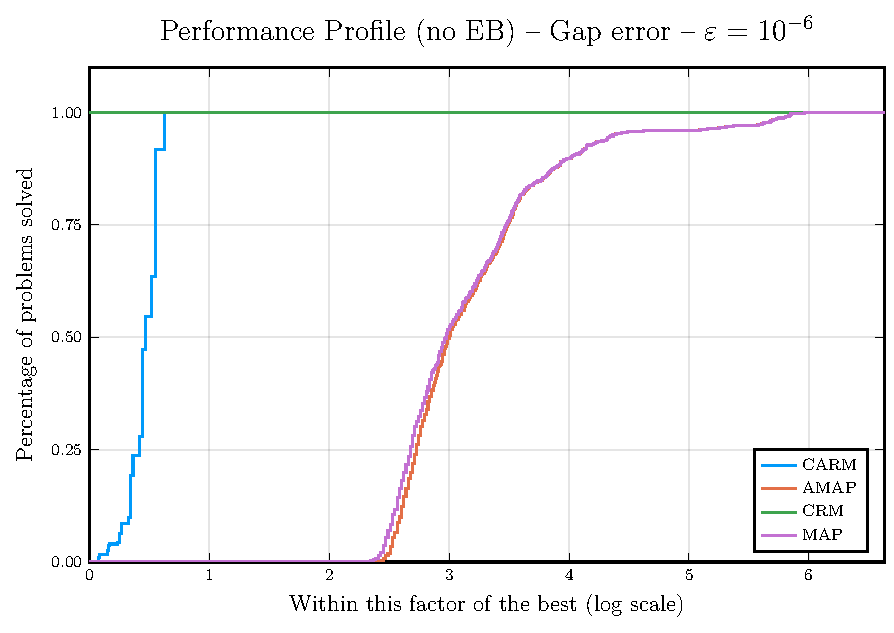
\includegraphics[scale=0.7]{fig1}
	\caption{Experiments with epigraph of a quadratic function and an affine subspace, without error bound - CARM, AMAP, CRM and MAP}
	\label{fig:perprof no EB 1}
\end{figure}

In the absence of an error bound, CARM perform exceptionally well, with a performance comparable to CRM's, which outperforms all the other algorithms. AMAP and MAP perform very similarly, with AMAP performing only slightly worse, both requiring at least twice the number of iterations required by CRM to in every problem and also being considerably outperformed by CARM.

Removing CRM from the comparison, in \cref{fig:perprof no EB 2} we can clearly see that CARM was considerably better than MAP and AMAP in all problems.
\begin{figure}[h!]
	\centering
	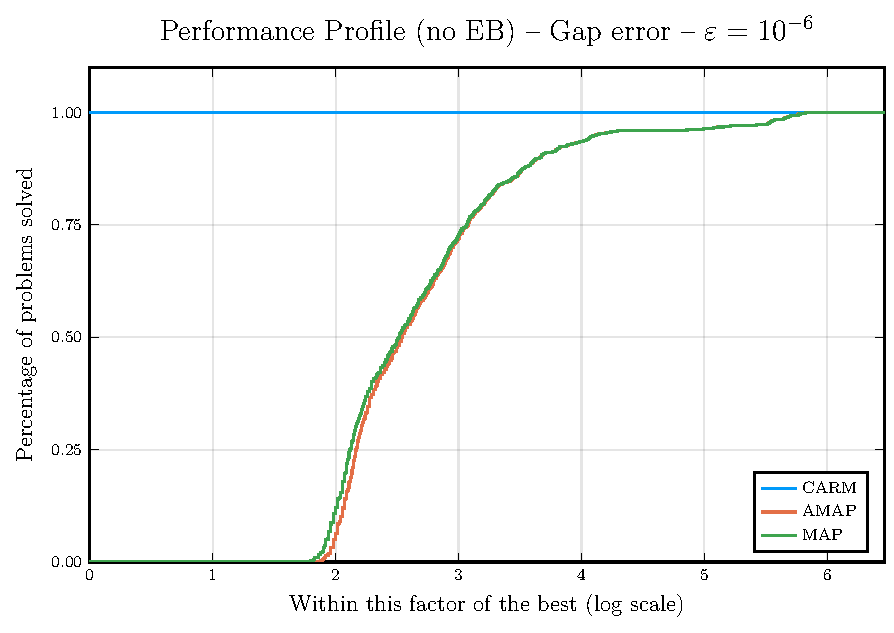
\includegraphics[scale=0.7]{fig2}
	\caption{Experiments with epigraph of a quadratic function and an affine subspace, without error bound - CARM, AMAP and MAP}
	\label{fig:perprof no EB 2}
\end{figure}
\newpage

To sum these results, we present descriptive statistics.
\begin{table}[h!]
\centering
\begin{tabular}{ccccc}
	\hline & mean & $\min$ & median & $\max$ \\
	\cline { 2 - 5 } CARM & 19.093 & 18 & 19.0 & 20 \\
	AMAP & 158.957 & 67 & 111.0 & 1171 \\
	CRM & 13.932 & 13 & 14.0 & 18 \\
	MAP & 157.083 & 64 & 109.0 & 1174 \\
	\hline
\end{tabular}
	\caption{Statistics of the experiments without error bound (in number of iterations)}
	\label{table:perprof no EB}
\end{table}

In the experiments with error bound, CRM remains the best performing method, in particular, outperforming MAP. This results is consistent with \cite{Behling:2020}, as $K$ is the epigraph of a (proper) convex function and $f$ satisfies the assumptions A1, A2, A3 and A4 shown in Section 4 of that paper to assure that CRM converges linearly, while MAP converges sublinearly. In \cref{fig:perprof EB 1} we can see how the presence of an error bound affects the performance of the algorithms.

\begin{figure}[h!]
	\centering
	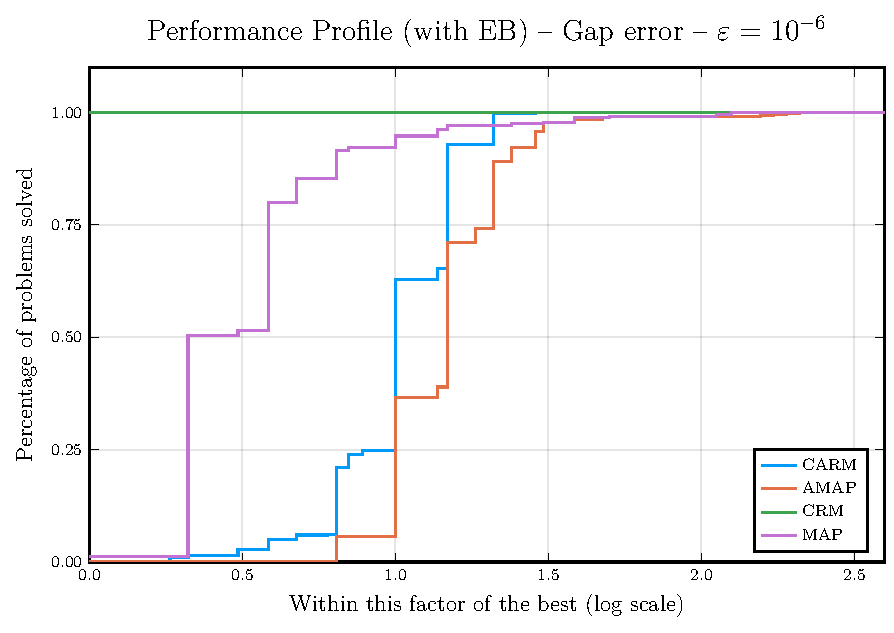
\includegraphics[scale=0.7]{fig1EB}
	\caption{Experiments with epigraph of a quadratic function and an affine subspace, with error bound - CARM, AMAP, CRM and MAP}
	\label{fig:perprof EB 1}
\end{figure}

\newpage

While MAP outperforms CARM in both cases, this comparison requires a closer look. Once again, we exclude CRM to take a clearer look into how CARM compares to MAP and AMAP.

\begin{figure}[h!]
	\centering
	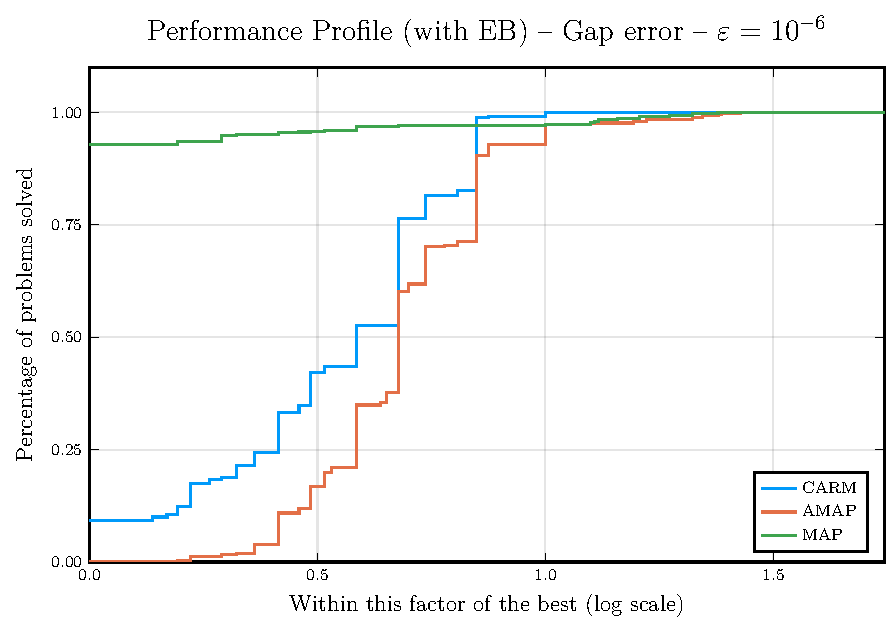
\includegraphics[scale=0.7]{fig2EB}
	\caption{Experiments with epigraph of a quadratic function and an affine subspace, with error bound - CARM, AMAP and MAP}
	\label{fig:perprof EB 2}
\end{figure}

While generally MAP outperforms CARM, CARM converged in at least as few iterations as MAP in 93 out of 1000 problems. We now remove MAP from the comparison to better visualize how CARM fares when compared with AMAP.

\begin{figure}[h!]
	\centering
	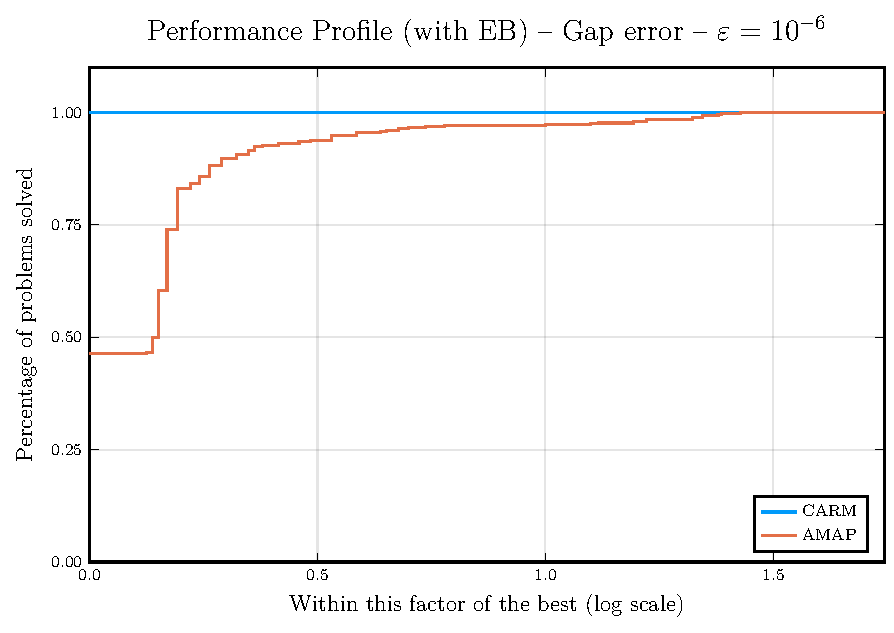
\includegraphics[scale=0.7]{fig3EB}
	\caption{Experiments with epigraph of a quadratic function and an affine subspace, without error bound - CARM and AMAP}
	\label{fig:perprof EB 3}
\end{figure}

The figure above makes it clear that CARM also outperforms AMAP handily with an error bound. We conclude this examination by presenting descriptive statistics for this error bound setting.

\begin{table}[h!]
	\centering
	\begin{tabular}{ccccc}
		\hline & mean & $\min$ & median & $\max$ \\
		\cline { 2 - 5 } CARM & 8.4 & 5 & 8.0 & 13 \\
		AMAP & 9.492 & 7 & 9.0 & 36 \\
		CRM & 4.15 & 4 & 4.0 & 7 \\
		MAP & 6.265 & 4 & 5.0 & 32 \\
		\hline
	\end{tabular}
	\caption{Statistics of the experiments with error bound (in number of iterations)}
	\label{table:perprof EB}
\end{table}

\newpage
\section{Final remarks}\label{sec:remarks}

We have extended results concerning the circumcentered-reflection method (CRM) by employing outer-approximate projections within a method we called CARM. In our numerical experiments, we see that CARM performs competitively with CRM. In the future, we hope to provide more interesting numerical experiments, such as when exact projections are unavailable, and more specific applications. In particular, we hope that CARM would perform well when compared with Combettes' Extrapolated Method of Parallel Subgradient Projections (EMOPSP) \cite{Combettes:1996} in an image recovery application.

We would also like to investigate the use overrelaxations onto outer-approximate projections as means of accelerating CARM and AMAP. Preliminary exploratory tests have been favorable, in that sense. Though it would require more complex calculations and perhaps stronger hypotheses, we also believe that outer-approximate projections could be used for projection methods outside of a product space formulation, where the availability of exact projections onto the affine subspace helps very much with proving the convergence.

\newpage
% \section{References}
\bibliographystyle{siamplain}

\bibliography{refs}

% \newpage
%\appendix
%\section{Appendix}


\end{document}
